%Dies ist die Hauptseite des Dokumentes. Es werden u. a. alle Kapitel,
%Einstellung im Header eingebunden.  Veränderungen müssen in folgenden Dateien
%vorgenommen werden:
      %- config.tex
      %- Versionsübersicht
      %- einzelne Kapitel (evtl. erweitern)

%Hier sind alle Einstellungen enthalten, die sich auf das Seiten- und
%Dokumentenlayout beziehen

\documentclass[
  11pt,                   % Schriftgröße
  DIV12,
  german,                 % für Umlaute, Silbentrennung etc.
  oneside,                % einseitiges Dokument
  titlepage,              % es wird eine Titelseite verwendet
  parskip=half,           % Abstand zwischen Absätzen (halbe Zeile)
  headings=normal,        % Größe der Überschriften verkleinern
  captions=tableheading,  % Beschriftung von Tabellen unterhalb ausgeben
  final                   % Status des Dokuments (final/draft)
]{scrreprt}               %


%------Ändern von Schriftschnitten - (Muss ganz am Anfang stehen !) ------------
\usepackage{fix-cm}


%------Umlaute -----------------------------------------------------------------
%   Umlaute/Sonderzeichen wie äüöß können direkt im Quelltext verwenden werden.
%    Erlaubt automatische Trennung von Worten mit Umlauten.
\usepackage[T1]{fontenc}
\usepackage[utf8]{inputenc}

%------Anpassung der Landessprache----------------------------------------------
\usepackage[ngerman]{babel}

%------Einfache Definition der Zeilenabstände und Seitenränder------------------
\usepackage{geometry}
\usepackage{setspace}

%------Schriftgrößenanpassung von einzelnen Textpassagen------------------------
\usepackage{relsize}

%------Trennlinien in Kopf- und Fusszeile
\usepackage[headsepline, footsepline, ilines]{scrpage2}

%------Grafiken und Farben -----------------------------------------------------
\usepackage{xcolor}
\usepackage{graphicx}

%------Packet zum Sperren, Unterstreichen und Hervorheben von Texten------------
\usepackage{soul}

%------ergänzende Schriftart----------------------------------------------------
\usepackage{helvet}

%------Lange Tabellen-----------------------------------------------------------
\usepackage{longtable}
\usepackage{array}
\usepackage{ragged2e}
\usepackage{lscape}

%------PDF-Optionen-------------------------------------------------------------
\usepackage[
  bookmarks,
  bookmarksopen=true,
  colorlinks=true,
  linkcolor=black,        % einfache interne Verknüpfungen
  anchorcolor=black,      % Ankertext
  citecolor=black,        % Verweise auf Literaturverzeichniseinträge im Text
  filecolor=black,        % Verknüpfungen, die lokale Dateien öffnen
  menucolor=black,        % Acrobat-Menüpunkte
  urlcolor=black,         % Farbe für URL-Links
  backref,                % Zurücktext nach jedem Bibliografie-Eintrag als
                          % Liste von Überschriftsnummern
  pagebackref,            % Zurücktext nach jedem Bibliografie-Eintrag als
                          % Liste von Seitenzahlen
  plainpages=false,       % zur korrekten Erstellung der Bookmarks
  pdfpagelabels,          % zur korrekten Erstellung der Bookmarks
  hypertexnames=false,    % zur korrekten Erstellung der Bookmarks
  linktocpage             % Seitenzahlen anstatt Text im Inhaltsverzeichnis verlinken
  ]{hyperref}






      % enthält eingebundene Packete

%------Seitenränder-------------------------------------------------------------
\geometry{verbose,                     % zeigt die eingestellten Parameter beim
                                       % Latexlauf an
      paper=a4paper,                   % Papierformat
      top=25mm,                        % Rand oben
      left=25mm,                       % Rand links
      right=25mm,                      % Rand rechts
      bottom=45mm,                     % Rand unten
      pdftex                           % schreibt das Papierformat in die
                                       % Ausgabe damit Ausgabeprogramm
                                       % Papiergröße erkennt
  }

%Seitenlayout
\onehalfspace        % 1,5-facher Abstand

%------Kopf- und Fußzeilen -----------------------------------------------------
\pagestyle{scrheadings}

%------Kopf- und Fußzeile auch auf Kapitelanfangsseiten ------------------------
\renewcommand*{\chapterpagestyle}{scrheadings}

%------Schriftform der Kopfzeile -----------------------------------------------
\renewcommand{\headfont}{\normalfont}

%----Spezielle Befehle
\newcommand{\lfk}[1]{$\langle LF#1\rangle$}

%----Farben
\definecolor{tubsRed}{cmyk}{0.1,1.0,0.8,0.0}
\definecolor{tuRed}{cmyk}{0.1,1.0,0.8,0.0}

%------Kopfzeile----------------------------------------------------------------
\setheadsepline{1pt}[\color{tuRed}]
\setlength{\headheight}{21mm}        % Höhe der Kopfzeile
\ihead{\large{\textsc{\praktikumTitel}}\\    % Text in der linken Box
       \small{\projektTitel}}
\chead{}                            % Text in der mittleren Box

%----Fusszeile
\setfootsepline{1pt}[\color{tuRed}]
\cfoot{}                            % Text in mittlerer Box
\ofoot{\pagemark}                    % Seitenzahl in rechter Box



%------Labels mit eigenem Text für \ref ----------------------------------------
\makeatletter
\def\namedlabel#1#2{\begingroup
#2%
\def\@currentlabel{#2}%
\phantomsection\label{#1}\endgroup
}
\makeatother


%------Neue Environments -------------------------------------------------------

\newcommand{\refsetcounter}[2]{\setcounter{#1}{#2}\addtocounter{#1}{-1}\refstepcounter{#1}}

%Funktion im Pflichtenheft
\newcounter{functioncount} 
\newenvironment{function}[2]{\refsetcounter{functioncount}{#1}\large\textbf{\sffamily{#2 }}\namedlabel{F#1}{$\langle F#1\rangle$}\normalsize\begin{description}\setlength{\itemsep}{-5pt}}{\end{description}}

%Daten im Pflichtenheft
\newcounter{datacount} 
\newenvironment{data}[2]{\refsetcounter{datacount}{#1}\textbf{#2} \namedlabel{D#1}{$\langle D#1\rangle$}\\}{}

%Kriterien im Pflichtenheft
\newcounter{mustcount} 
\newcommand{\must}[2]{\refsetcounter{mustcount}{#1}\namedlabel{RM#1}{$\langle RM#1\rangle$} #2\\}

\newcommand{\should}[2]{\refsetcounter{datacount}{#1}\namedlabel{RS#1}{$\langle RS#1\rangle$} #2\\}

\newcommand{\could}[2]{\refsetcounter{datacount}{#1}\namedlabel{RC#1}{$\langle RC#1\rangle$} #2\\}

\newcommand{\wont}[2]{\refsetcounter{datacount}{#1}\namedlabel{RW#1}{$\langle RW#1\rangle$} #2\\}

%Qualitätsanforderungen im Pflichtenheft
\newcommand{\qualityReq}[2]{\refsetcounter{datacount}{#1}\namedlabel{Q#1}{$\langle Q#1\rangle$} #2\\}

% Benutzeroberflächen im Pflichtenheft
\newcounter{uicount}
\newenvironment{ui}[2]{\refsetcounter{uicount}{#1}\textbf{#2} \namedlabel{UI#1}{$\langle UI#1\rangle$}\\}{}

% Klassen
\newcounter{classcount}
\newenvironment{class}[2]{\refsetcounter{classcount}{#1}\textbf{#2}\namedlabel{CL#1}{$\langle CL#1\rangle$}\begin{description}\setlength{\itemsep}{-5pt}}{\end{description}}

% Entitäten
\newcounter{entitycount}
\newenvironment{entity}[2]{\refsetcounter{entitycount}{#1}\textbf{#2} \namedlabel{E#1}{$\langle E#1\rangle$}\\}{}

% Component
\newcounter{componentcount}
\newenvironment{component}[2]{\refsetcounter{componentcount}{#1}\textbf{Komponente \namedlabel{C#1}{$\langle C#1\rangle$}: #2}\\}{}

% Interface
\newcounter{interfacecount}
\newenvironment{interface}[2]{\refsetcounter{interfacecount}{#1}\textbf{Schnittstelle \namedlabel{I#1}{$\langle I#1\rangle$}: #2}\\}{}

% Testfall
\newcounter{testcasecount}
\newenvironment{testcase}[2]{\clearpage\refsetcounter{testcasecount}{#1}\subsection{Testfall $\langle T#1\rangle$ - #2}\label{T#1}\begin{description}\setlength{\itemsep}{-5pt}}{\end{description}}
          % Diese Datei enthält alle
                                          % Layouteinstellungen
\newcommand{\dokumentTitel}{Systemspezifikation 2}
% Definition von globalen Parametern, die derzeit auf der Titelseite und in der
% Kopfzeile verwendet werden. Der in <> gesetzte Text ist zu verändern.

\newcommand{\praktikumTitel}{Das Gro\ss{}e SQL-Spiel}
\newcommand{\projektTitel}{The SQL-Alchemist}
\newcommand{\institut}{
	Institut f\"ur Informationssysteme\\
	Prof. Dr. Wolf-Tilo Balke\\
	M\"uhlenpfordtstra\ss{}e 23, 2.OG\\
	D-38106 Braunschweig\\
}
\newcommand{\institutsLogo}{common/ISF_Logo.pdf}
\newcommand{\betreuer}{Jan-Christoph Kalo}

\externaldocument{Pflichtenheft}

%------Beginn des Gesamtdokumentes----------------------------------------------
\begin{document}

%------Eingebundene Seiten, Verzeichnisse bzw. Kapitel--------------------------
% Dies ist die Titelseite.
% Die Ausgabe darf 1 Seite nicht überschreiten, also ggf. Abstände anpassen
% Die Angabe in [...] gibt den Abstand nach der entsprechenden Zeile an.


%----Stil dieser Seite----------------------------------------------------------
\thispagestyle{plain}      % Kopfzeile bleibt leer

%----Beginn der Titelseite------------------------------------------------------
\begin{titlepage}

%----eingebundenes Logo der TU--------------------------------------------------
%\setlength{\unitlength}{1mm}
%  \begin{picture}(00,00)(+25,-04)
%  	\color{tuRed}
%    \put(055,006){\line(1,0){150}}
%    \put(005,000){
\includegraphics[width=6.3cm]{common/TUBraunschweig_4C.pdf}}
%    \put(150,010){\includegraphics[width=8cm,height=2.4cm,keepaspectratio]{\institutsLogo}}
%  \end{picture}\\[5ex]
%\hspace*{-2cm}


\vspace*{-3.8cm}
\hspace*{-2cm}\begin{minipage}{1.25\textwidth}

\includegraphics[width=6.3cm]{common/TUBraunschweig_4C.pdf}\setlength{\unitlength}{1mm}\begin{picture}(00,00)(0,0)\color{tuRed}\put(000,004){\line(1,0){150}}\end{picture}%\hfill
\parbox[b]{0.68\textwidth}{\hfill\includegraphics[width=8cm,height=2.4cm,keepaspectratio]{\institutsLogo}\\~}
\end{minipage}


~\\[4ex]

%----zentrierte Ausrichtung über die gesamte Seite----------------------------
\begin{center}

%----Titel des Praktikum (\praktikumTitel in newComments zu verändern)--------
{\relsize{4}{\textbf{\textsc{\praktikumTitel}}}}\\[4ex]

%----Titel des Teilprojektes (\projektTitel in newComments verändern)---------
{\relsize{3}{\textbf{\textsc{\projektTitel}}}}\\[4ex]

Software-Entwicklungspraktikum (SEP)\\
Sommersemester 2015\\[4ex]

{\relsize{3}{\textbf{\dokumentTitel}}}\\[2ex]

%----Daten des Auftraggebers
Auftraggeber:\\
Technische Universität Braunschweig\\
\institut[2ex]
Betreuer: \betreuer\\[2ex]

Auftragnehmer:\

% ----Tabelle der Praktikumsteilnehmer------------------------------------------
\begin{tabular}{l<{\hspace{20mm}} l<{\hspace{21mm}}}\\

  Name                   &   E-Mail-Adresse\\      % Zeilenüberschift

  \hline                    % Linie unterhalb der Zeilenüberschrift

  %----Nachfolgend alle Namen und E-Mail-Adressen der Teilnehmer einfügen
 
 Gabriel Ahlers &  g.ahlers@tu-braunschweig.de\\
 Majid Dashtiepielehroud &  m.dashtiepielehroud@tu-braunschweig.de\\
 Ronja Friebe &  r.friebe@tu-braunschweig.de\\  
 Stefan Hanisch &  stefan.hanisch@tu-braunschweig.de\\  
 Fabio Luigi Mazzone & f.mazzone@tu-braunschweig.de\\  
 Nicole Naczk &  n.naczk@tu-braunschweig.de\\  
 Denis Nagel &  denis.nagel@tu-braunschweig.de\\  
 Luca Porcello &  l.porcello@tu-braunschweig.de\\  
 Christian Reineke &  c.reineke@tu-braunschweig.de\\  
 Christian Sander &  christian.sander@tu-braunschweig.de\\  
 Carl Schiller &  c.schiller@tu-braunschweig.de\\  
 Levent Muzaffer \"Uner &  l.uener@tu-braunschweig.de\\  
 S\"oren van der Wall &  s.van-der-wall@tu-braunschweig.de\\  
 Daniel Wolfram &  d.wolfram@tu-braunschweig.de\\  


\end{tabular}

%Zur Vereinheitlichung sollten hier die TU Braunschweig Emailadressen benutzt werden. % enthält Tabelle der Praktikumsteilnehmer

\vfill
Braunschweig, \today

\end{center}
\end{titlepage}
                      % Titelseite
%!TEX root = ../Systementwurf2.tex

%Diese Datei dient der Versionskontrolle. Sie ist vollständig zu bearbeiten.

%----Überschrift------------------------------------------------------------
{\relsize{2}\textbf{Versionsübersicht}}\\[2ex]

%----Start der Tabelle------------------------------------------------------
\begin{longtable}{|m{1.78cm}|m{1.59cm}|m{2.86cm}|m{1.9cm}|m{5.25cm}|}

  \hline                                              % Linie oberhalb

  %----Spaltenüberschriften------------------------------------------------
  \textbf{Version}  &    \textbf{Datum}  &    \textbf{Autor}  &
  \textbf{Status}   &    \textbf{Kommentar}       \\  %Spaltenüberschrift
  \hline                                              % Gitterlinie

  %----die nachfolgeden beiden Zeilen so oft wiederholen und die ... mit den
  %    entsprechenden Daten zu füllen wie erforderlich
%   0.1    &    13.05.2014    &    F. Heymann   &        &   
%  Kapitel Datenmodell hinzugefügt\\
%  \hline
%   0.2    &    14.05.2014    &    P. Dittrich  &        &   
%  Kapitel Produktfunktionsanalyse und Glossar hinzugefügt\\
%  \hline 
%   0.3    &    14.05.2014    &    C. Sontag   &        &   
%  Einleitung hinzugefügt\\
%  \hline 
%   0.4    &    22.05.2014    &    C. Sontag   &        &   
%  Einleitung bearbeitet\\
%  \hline 
%   0.5    &    22.05.2014    &    D. Klose   &        &   
%  Kriterienerfüllung hinzugefügt\\
%  \hline 
%	 0.5    &    23.05.2014    &    A. Reiss   &        &   
%  Kapitel 3.1 hinzugefügt\\
%  \hline 
%	0.5    &    23.05.2014    &    A. Reiss   &        &   
%  Kapitel 3.2 hinzugefügt\\
%  \hline 
%    0.6    &    23.05.2014    &    P. Dittrich   &        &   
%  Einleitung leicht überarbeitet\\
%  \hline 
%	 0.6    &    23.05.2014    &    A. Reiss   &        &   
%  3.1/3.2 überarbeitet 3.3 hinzugefügt\\
%  \hline 
%	 0.6    &    23.05.2014    &    A. Reiss   &        &   
%  Kapitel 3 überarbeitet\\
%  \hline
%  	 0.7    &    26.05.2014    &    C. Sontag   &        &   
%  Kapitel 3.2 überarbeitet\\
%  \hline
%  0.8    &    28.05.2014    &    N. Widdecke   &   vorgelegt &  Layout und Rechtschreibkorrektur  \\
%  \hline 
  1.0    &    28.05.2014    &    Auftragnehmer &  vorläufig &  erster Entwurf des Dokuments mit den Kapiteln 1--4, 8 und 9\\
  \hline 
  2.0    &    28.05.2014    &    Auftragnehmer &  vorläufig &  Korrekturen\\
  \hline
  3.0 	& 05.07.2014 & Auftragnehmer & vorläufig & Einfügen der Kapitel 5--7\\
  \hline
    4.0 	& 05.07.2014 & Auftragnehmer & vorgelegt & Korrekturen \\
  \hline

%----Ende der Tabelle------------------------------------------------------
\end{longtable}

%Status: "`in Bearbeitung"', "`vorgelegt"', "`vorläufig"', "`abgenommen"' oder "`abgelehnt"'\\
%Kommentar: hier eintragen, was und wo geändert bzw. ergänzt wurde (z.B. Kapitel )
%
%
%Hinweis zum Template:
%Dieses Template enth\"ult Hinweise, die alle kursiv geschrieben sind. Alles
%Kursivgeschriebene ist selbstverst\"andlich bei Abgabe zu entfernen sind.
%Angaben in <\ldots> sind mit dem entsprechendem Text zu füllen.  Überzählige
%Kapitel, d.h. Kapitel, die nicht bearbeitet werden m\"ussen, da sie nicht der
%Aufgabenstellung entsprechen, bitte entfernen.
%
%Aufgabe des Grobentwurfs (Systemspezifikation 1): Aufgabe dieses Dokumentes ist es, die Architektur des
%Systems zu beschreiben und die daraus resultierenden Pakete durch die
%Definition von Schnittstellen zu Komponenten auszubauen.
%
%Aufgabe des Feinentwurfs (Systemspezifikation 2): Der Feinentwurf dokumentiert die klassischen Entwurfsentscheidungen wie z.B. Verwendung bestimmter Bibliotheken oder Entwurfsmuster. Darueber hinaus bildet der Feinentwurf die Grundlage der Implementierung, d.h. anhand
%dieses Dokumentes muss jeder Softwareentwickler in der Lage sein, das Produkt
%zu entwickeln. Es ist also auf Vollständigkeit der Dokumentation zu
%achten.
       % Versionsübersicht

\tableofcontents                          % Inhaltsverzeichnis wird automatisch
                                          % generiert
\listoffigures                            % ebenso das Abbildungsverzeichnis

%----Kapitel des Feinentwurfs, die mit Inhalt zu füllen sind--------------------
%!TEX root = ../Testspezifikation.tex

\chapter{Einleitung}

Einer der wichtigsten Aspekte bei der Entwicklung von Software ist das ausführliche Testen des Programms. Dabei müssen für diese Software alle Softwarebestandteile, auf ihre Funktionsweise, Ausfallsicherheit und Bedienbarkeit getestet werden. Gleichzeitig dient das Testen der Qualitätssicherung der Applikation. Dies ist speziell bei dieser Software wichtig, da sie den Lehrbetrieb der Veranstaltung \glqq Relationale Datenbanksysteme 1 \grqq~unterstützen und einen Teil des Hausaufgabenablaufs übernehmen soll.

Aus diesem Grund wird auch der SQL-Alchemist umfangreichen Tests unterzogen um einen reibungslosen Betrieb, während der späteren Nutzung zu gewährleisten. Insbesondere da das Programm später vorlesungsunterstützend eingesetzt werden soll und Einfluss auf die erfolgreiche Bearbeitung der Hausaufgaben der Studenten hat, ist es umso wichtiger, dass keine unvorhergesehenen Fehler auftreten, welche durch ein frühes Testen hätten verhindert werden können.

In diesem Dokument wird ausführlich auf die einzelnen Bereiche der Software eingegangen, welche verschiedenen Tests unterzogen werden müssen. Dabei wird auch die genaue Vorgehensweise der Testläufe näher beschrieben. 



%Wie in der Vorlesung erwähnt, ist das Testen von Software unerlässlich und darf
%bei keinem Softwareentwicklungsprozess fehlen.

%Diese Testdokumentation ist angelehnt an den IEEE 829-Standard, der als
%der bekannteste Standard für Software-Testdokumentationen gilt. 
%Der Standard definiert eine Menge von Testdokumenten
%und beschreibt deren Inhalte. 

%In diesem Kapitel soll kurz allgemein beschrieben werden, welche Software getestet wird, 
%welchen Qualitätsanforderungen sie genügt und welche Standards unter umständen zu beachten sind.
% (Umfang ca. $\frac{1}{3}$ bis 1 Seite)

%\textbf{Hinweis zu den Templates:}\\
%Dieses Template enthält Hinweise und Beispiele, die selbstverständlich zu entfernen sind.
% Angaben in <...> sind mit dem entsprechendem Text zu füllen.

%\textbf{Kapitel die bereits in der Abnahmetestspezifikation bearbeitet wurden, müssen hier nicht erneut
% bearbeitet werden. Es sollten jedoch die Annotationen umgesetzt worden sein.
% Es sollen also Kapitel 4-5 neu erarbeitet und Kapitel 2.1 überarbeitet werden.}


%\textbf{Dieses Kapitel kann aus der Abnahmetestspezifikation übernommen werden, 
%sollte jedoch die Bearbeitung der Annotationen beinhalten.}
%!TEX root = ../TechnischerEntwurf.tex

\chapter{Analyse der Produktfunktionen}\label{chap:analyse}

Im Folgenden werden die im Pflichtenheft benannten Funktionen näher beschrieben und erkl\"art. Dabei wird davon ausgegangen, dass der User sich in dem Interface befindet, in dem er die erklärte Funktion initiieren kann.

Des Weiteren ist zu erkennen, dass, jedes mal wenn das Back-End nach der Registration oder dem Login aktiv wird, es zuerst einen \glqq checkSession()\grqq -Methodenaufruf startet. Dies ist die Überprüfung des Back-Ends, ob es selbst den User kennt, ob er die gebrauchten Rechte für die Aktion hat und ob die Aktion auch auf die zum User gehörenden Daten ausgeführt wird.

\newpage
\section{Analyse von Funktionalität <F10>: <Nutzer registrieren>}
\label{sequence_f10}
\begin{figure}[htb]
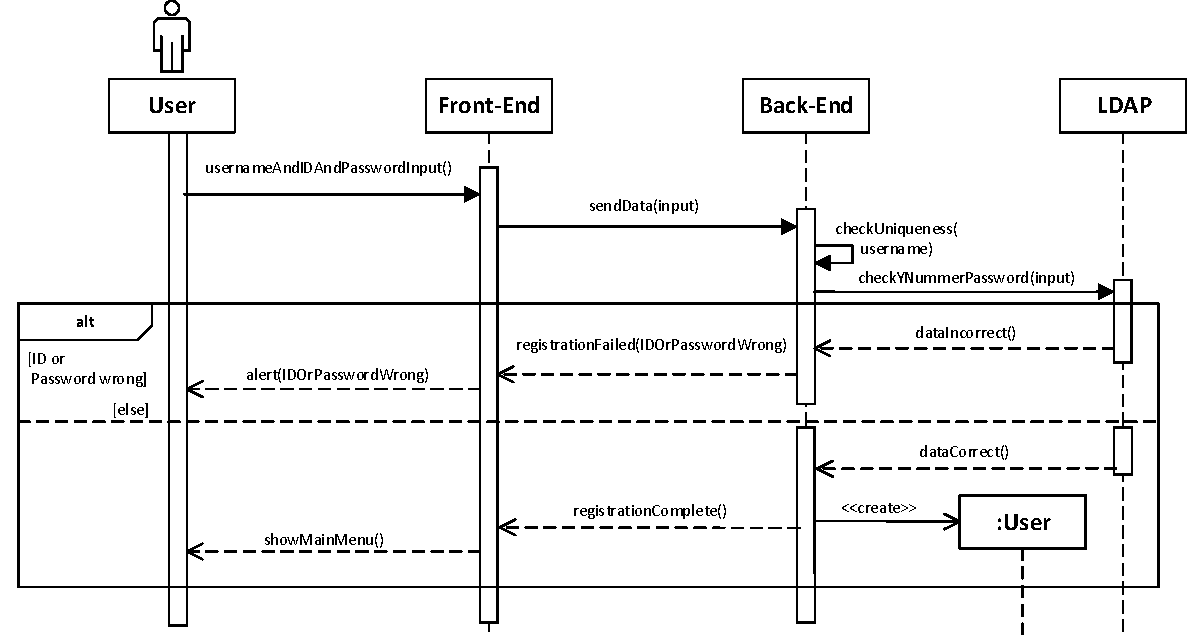
\includegraphics[width=1\textwidth]{figures/sequenz_F10.pdf}
\caption{Sequenzdiagramm zur Registrierung}
\end{figure}

In Diagramm \ref{sequence_f10} wird der Vorgang der Registrierung beschrieben.

Dafür muss der User zuerst einen Username, eine E-Mail-Adresse oder seine y-Nummer (insgesamt ID genannt) und ein Passwort (im Falle einer y-Nummer das zur y-Nummer gehörende Passwort) angeben. Diese Eingaben werden dann an das Back-End übertragen. Hier wird zuerst geprüft ob der Username schon vergeben ist. Sollte das der Fall sein, wird dies dem User mitgeteilt und er muss einen neuen Username angeben.
Wenn der Username noch nicht vergeben war, wird, im Falle dass es sich bei der ID um eine E-Mail-Adresse handelt, geprüft, ob diese schon vorhanden ist. Wenn die ID eine y-Nummer ist, wird diese, inklusive des eingegebenen Passworts, an das \glqq LDAP\grqq ~geschickt und dort überprüft. Sollte der jeweils zutreffende Schritt fehlschlagen, muss der User seine Eingaben ändern, beziehungsweise korrigieren und der Prozess beginnt von vorn.

Sollte der Ablauf erfolgreich abgeschlossen worden sein, erstellt das Back-End ein neues User-Objekt, speichert dies in seiner Datenbank und gibt die Rückmeldung, dass die Registrierung erfolgreich gewesen ist. Der User wird dann in das Hauptmenü weitergeleitet.
%==================================================================

\newpage
\section{Analyse von Funktionalität <F20>: <Nutzer anmelden>}
\begin{figure}[h]
\centering
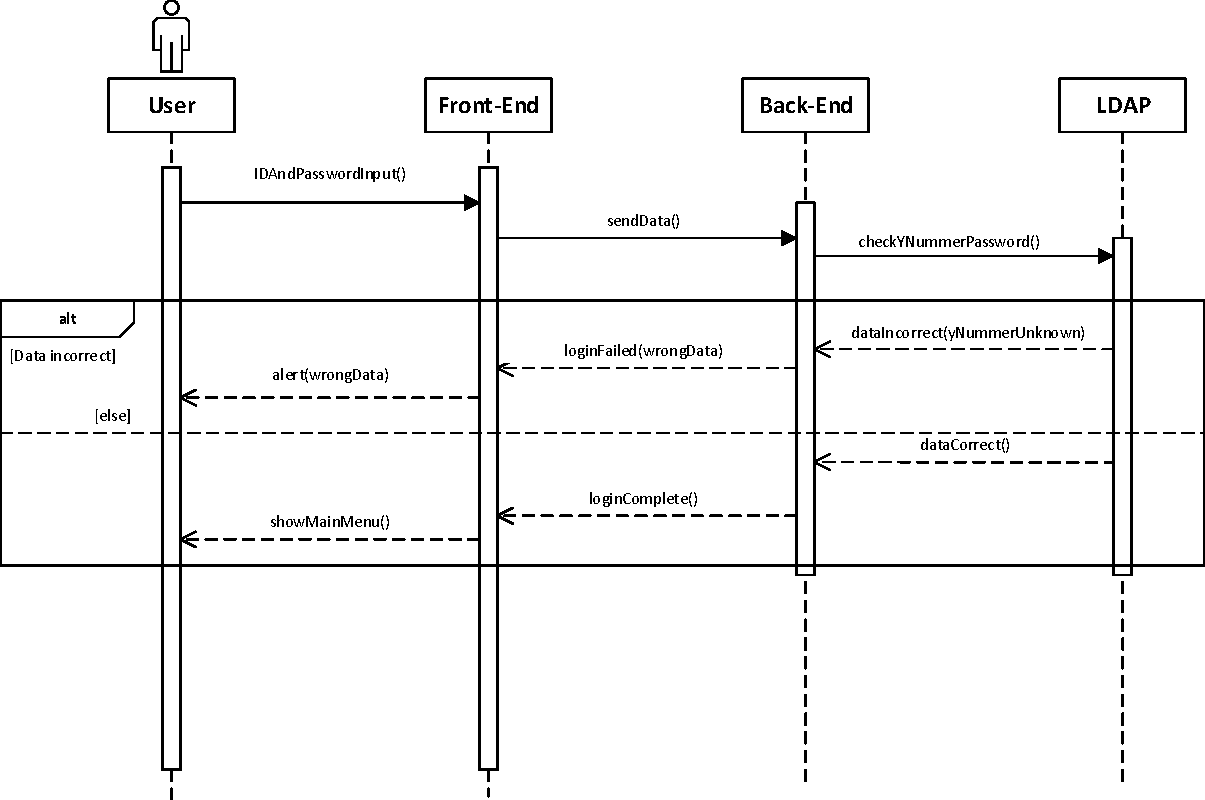
\includegraphics[width=1\textwidth]{figures/sequenz_F20.pdf}
\caption{Sequenzdiagramm zum Login}
\label{sequence_f20}
\end{figure}
Das Diagramm \ref{sequence_f20} beschreibt den Login-Vorgang. 

Hierbei muss der User die von ihm registrierte ID (siehe <F10>) und sein Passwort angeben. Diese werden, je nach Typ der ID, dann entweder mit der eigenen Datenbank verglichen, oder, sollte die ID eine y-Nummer sein, an das \glqq LDAP\grqq ~geschickt und dort überprüft.\\
Sollten die eingegeben Daten nicht korrekt sein, wird dies dem User mitgeteilt und er bekommt die Möglichkeit seine Eingaben zu korrigieren. Sind die Daten korrekt wird der User in das Hauptmenü weitergeleitet.
%==================================================================

\newpage
\section{Analyse von Funktionalität <F30>: <Nutzer abmelden>}
\begin{figure}[h]
\centering
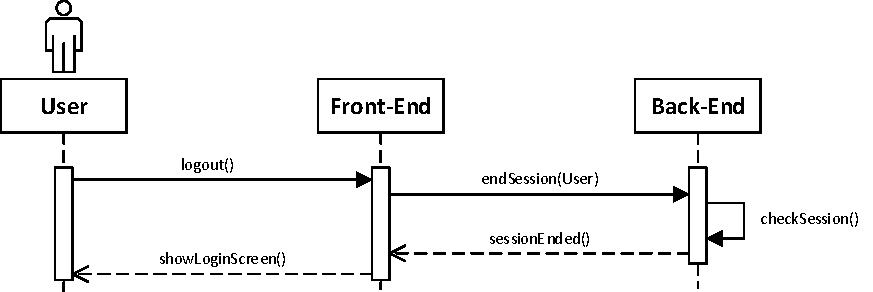
\includegraphics[width=1\textwidth]{figures/sequenz_F30.pdf}
\caption{Sequenzdiagramm zum Login}
\label{sequence_f30}
\end{figure}
Das Diagramm \ref{sequence_f30} beschreibt den Ablauf des Ausloggens.

Entscheidet sich der User dazu sich auszuloggen, wird diese Information an das Back-End gesendet. Dieses beendet die Session des Users. Ist das geschehen wird eine Benachrichtigung an das Front-End gesendet und der User wird zurück zum Login-Screen geleitet.
%==================================================================

\newpage
\section{Analyse von Funktionalität <F40>: <Profil einsehen>}
\begin{figure}[h]
\centering
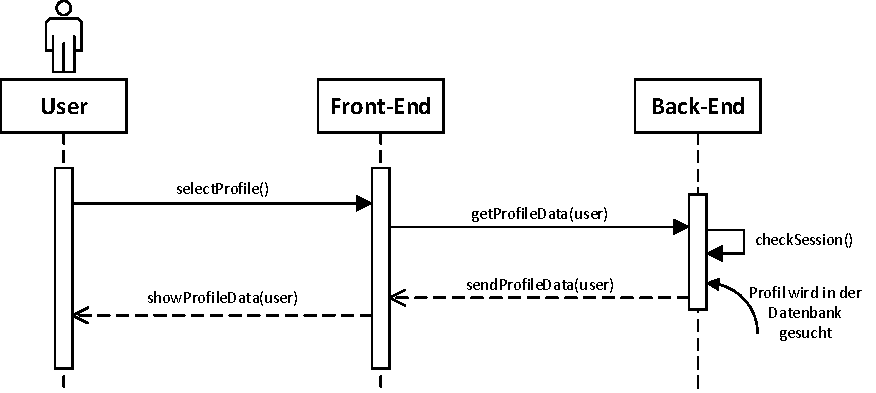
\includegraphics[width=1\textwidth]{figures/sequenz_F40.pdf}
\caption{Sequenzdiagramm zur Darstellung der Profilübersicht}
\label{sequence_f40}
\end{figure}
Das Diagramm  \ref{sequence_f40} zeigt was passiert, wenn man sich das eigene Userprofil anzeigen lassen möchte.

Um das Profil des Users anzuzeigen, werden zuerst die Userdaten vom Back-End angefordert. Das Back-End lädt dann die Profildaten aus den Userdaten und schickt diese zurück an das Front-End. Dort werden sie, für den User einsehbar, im Profil-Interface angezeigt.

%==================================================================

\newpage
\section{Analyse von Funktionalität <F60>: <Passwort ändern>}
\begin{figure}[h]
\centering
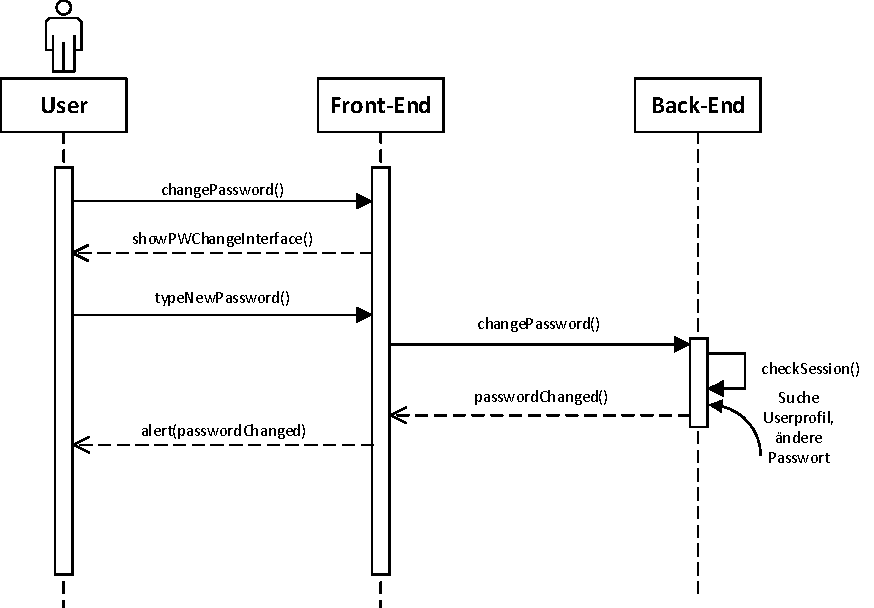
\includegraphics[width=1\textwidth]{figures/sequenz_F60.pdf}
\caption{Sequenzdiagramm zum Ändern des Passworts}
\label{sequence_f60}
\end{figure}
Das Diagramm \ref{sequence_f60} beschreibt das Ändern des Passwortes.

Das Ändern des Passwortes steht nur nicht-studentischen Nutzern zur Verfügung.
Entscheidet sich der Nutzer, sein Passwort zu ändern, kann er dies mit einem Klick auf den \glqq Change Password \grqq -Button tun. Zuerst muss er sein altes Passwort eingeben und im Anschluss kann er ein neues Password erstellen. Dies muss danach noch einmal bestätigt werden und wenn alles erfolgreich war, wird das geänderte Passwort an das Back-End geschickt und dort in den Nutzerdaten vermerkt. Sollte während des Vorgangs ein Fehler auftreten, bleibt das alte Passwort bestehen und der User wird darüber in Kenntnis gesetzt.
%==================================================================

\newpage
\section{Analyse von Funktionalität <F70>: <Avatar ändern>} 
\begin{figure}[h]
\centering
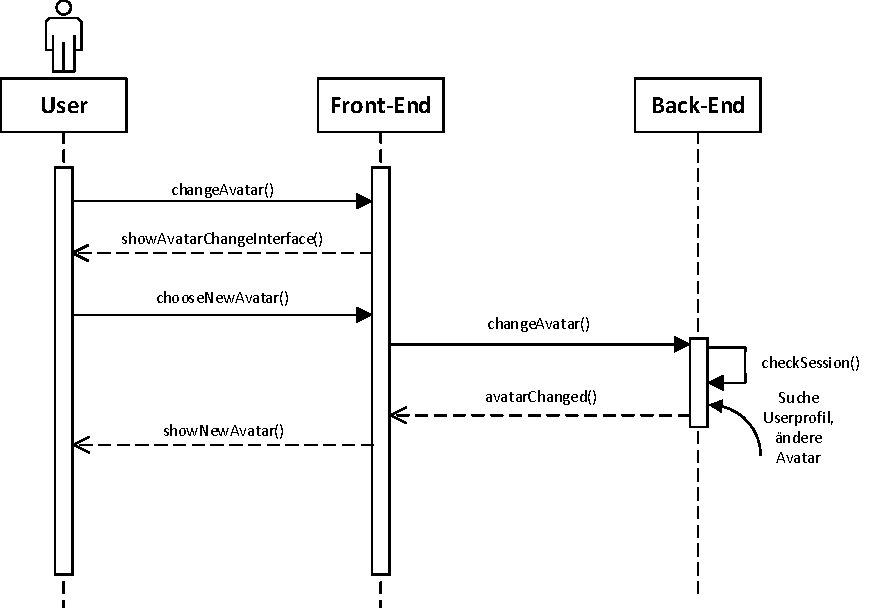
\includegraphics[width=1\textwidth]{figures/sequenz_F70.pdf}
\caption{Sequenzdiagramm zum Ändern des Avatars}
\label{sequence_f70}
\end{figure}
Das Diagramm \ref{sequence_f70} beschreibt das Ändern des Avatars.

Klickt der User auf den \glqq Change Avatar \grqq -Button, werden ihm alle seine verfügbaren Avatare angezeigt und er kann sich für einen entscheiden. Hat er dies getan wird die Änderung der Einstellung vermerkt, ans Back-End geschickt, dort gespeichert und dann, wieder zurück im Front-End, aktualisiert angezeigt.
%==================================================================

\newpage
\section{Analyse von Funktionalität <F80>: <Benutzer löschen>} 
\begin{figure}[h]
\centering
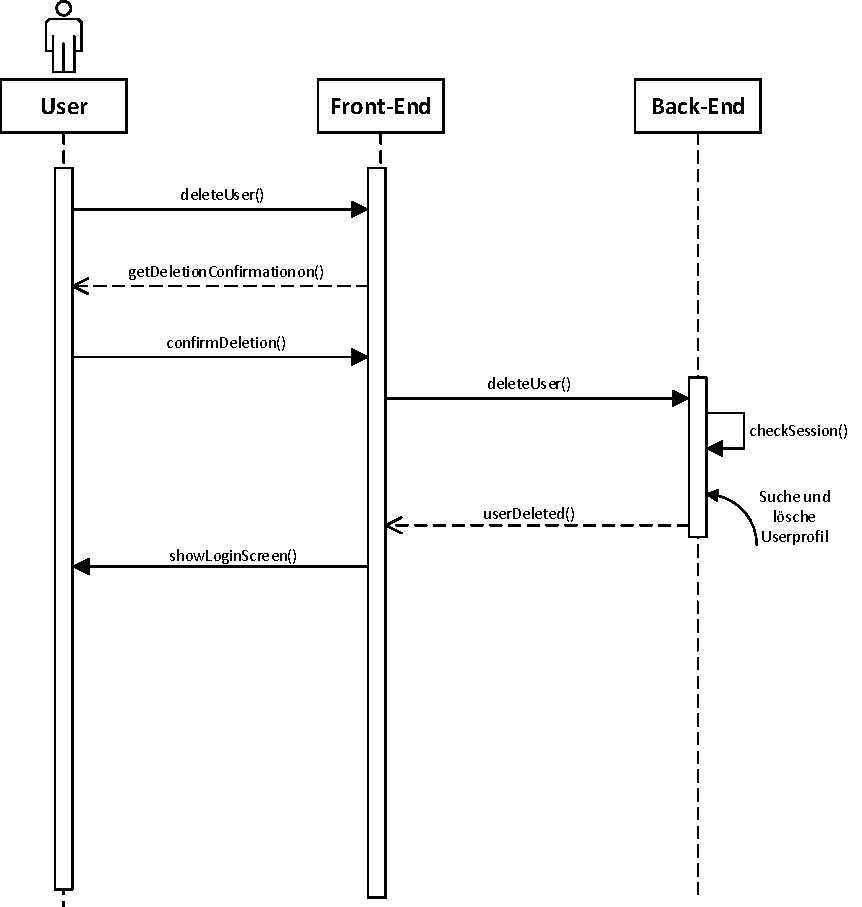
\includegraphics[width=0.9\textwidth]{figures/sequenz_F80.pdf}
\caption{Sequenzdiagramm zum Löschen des Benutzers}
\label{sequence_f80}
\end{figure}
Diagramm \ref{sequence_f80} zeigt, was passiert, wenn der User seinen Account löschen möchte.
Möchte der User sein Profil löschen, kann er dies im Settings-Interface tun, welches dementsprechend erst geladen werden muss. Wenn der User nun den \glqq Delete User\grqq -Button drückt, wird er erst noch einmal gefragt, ob er sein Profil wirklich löschen möchte. Beantwortet der User dies positiv, geht eine Mitteilung an das Back-End, wo das Profil gelöscht wird. Der User wird dann auf den Login-Screen geleitet, wo es ihm frei steht, sich wieder zu registrieren.
%==================================================================

\newpage
\section{Analyse von Funktionalität <F90>: <Audioeinstellungen bearbeiten>}
\begin{figure}[h]
\centering
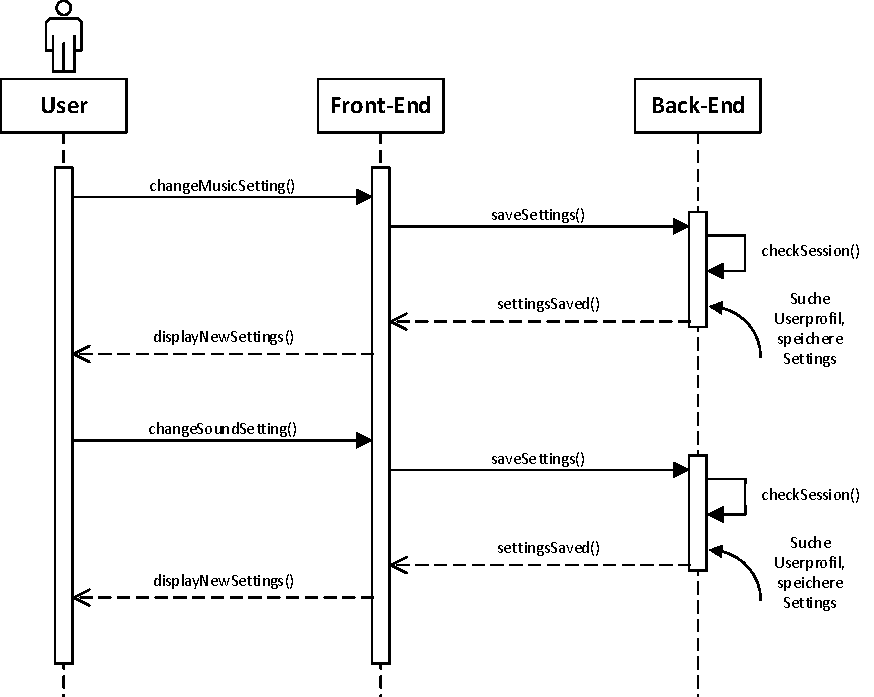
\includegraphics[width=0.9\textwidth]{figures/sequenz_F90.pdf}
\caption{Sequenzdiagramm zum Ändern der Audioeinstellungen}
\label{sequence_f90}
\end{figure}
Diagramm \ref{sequence_f90} zeigt, was passiert, wenn der User seine Audio-Optionen ändert.

Zum Ändern der Audiofunktionen stehen Knöpfe bereit, die sowohl die Hintergrundmusik (\glqq Music\grqq) als auch die Soundeffekte, wie Sprungsounds und Klicksounds,  aus-  beziehungsweise einstellen. Jegliche \"Anderung wird sofort ans Back-End gesendet, dort gespeichert und dann im Profil aktualisiert.
%==================================================================

\newpage
\section{Analyse von Funktionalität <F100>: <Spielstand zurücksetzen>}
\begin{figure}[h]
\centering
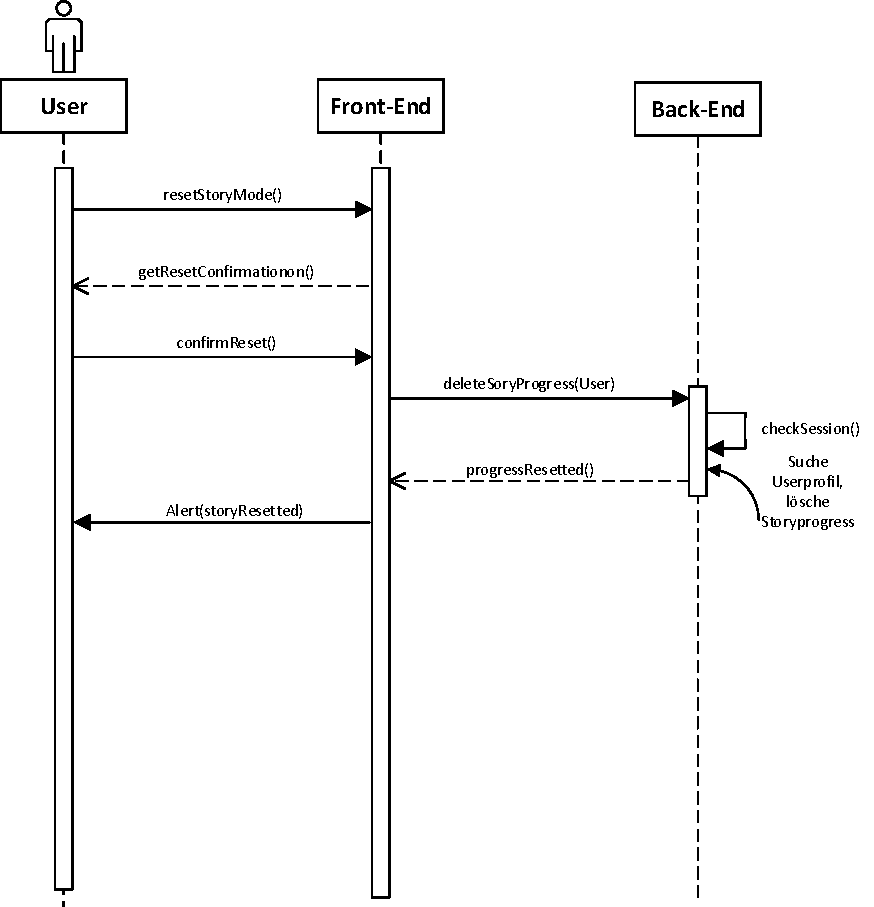
\includegraphics[width=0.9\textwidth]{figures/sequenz_F100.pdf}
\caption{Sequenzdiagramm zum Zurücksetzen des Spielstands}
\label{sequence_f100}
\end{figure}
Diagramm \ref{sequence_f100} beschreibt das Zurücksetzen des Storyfortschritts.

Der User kann per Knopfdruck seinen Story-Fortschritt zurücksetzen. Tut er dies, muss er vorher noch einmal seine Zustimmung zum Löschvorgang geben. Ist auch dies geschehen, wird die Anweisung zum Löschen des Storyfortschritts des Users an das Back-End geschickt und dort ausgeführt.
%==================================================================

\newpage
\section{Analyse von Funktionalität <F110>: <Tutorial spielen>}
\begin{figure}[h]
\centering
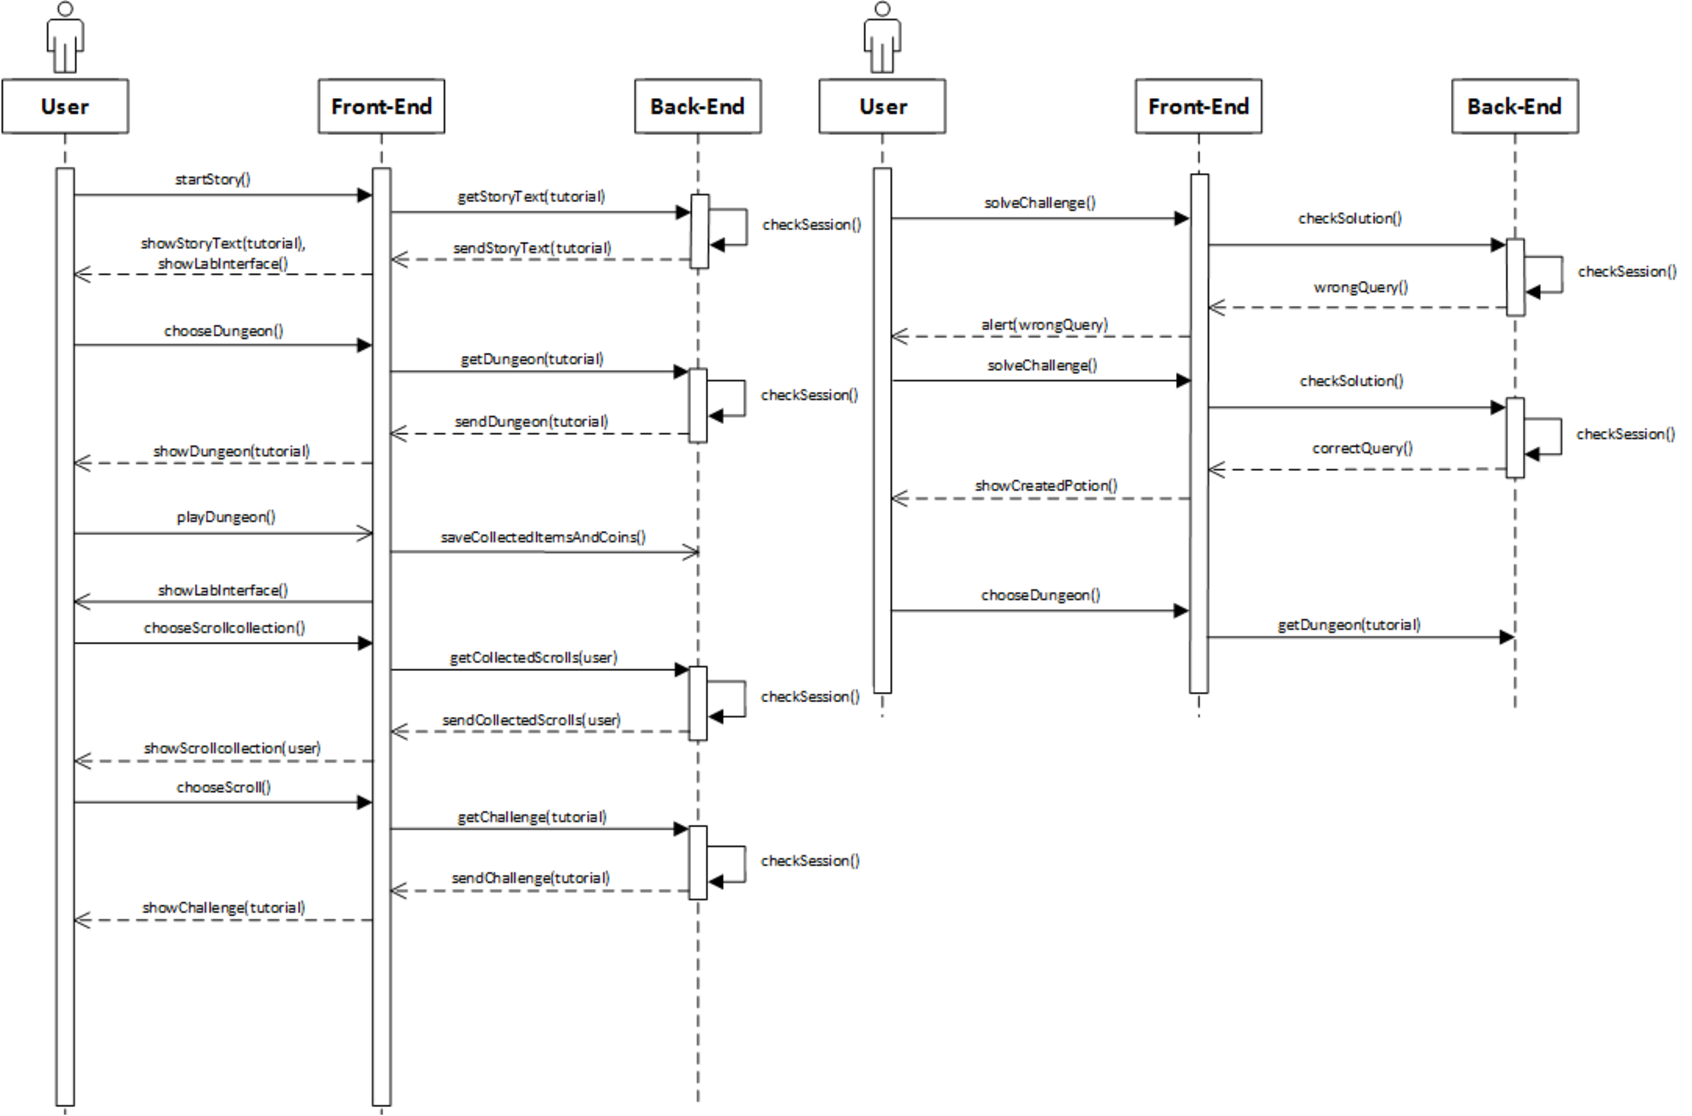
\includegraphics[width=1.0\textwidth]{figures/sequenz_F110.pdf}
\caption{Sequenzdiagramm für das Tutorial}
\label{sequence_f110}
\end{figure}
Diagramm \ref{sequence_f110} zeigt den Ablauf im Tutorial.

Wird das Tutorial gestartet, werden zuerst alle Tutorial-Texte vom Back-End angefordert. Diese werden dann, wenn benötigt, dem User angezeigt. Zuerst wird der User in den Dungeon geleitet. Dazu werden die Leveldaten vom Back-End geladen, sodass der User den Dungeon betreten und spielen kann. Hierbei kann er Schriftrollen (\glqq Scrolls\grqq) und Münzen (\glqq Lofi-Coins\grqq) einsammeln, was jeweils sofort ans Back-End gesendet und dort im Story-Progress bzw. in den Profildaten gespeichert wird.
Scheitert der User an einer Hürde im Dungeon, bekommt er zuerst einen Game-Over-Screen angezeigt, auf dem zu sehen ist, was er eingesammelt hat und wird dann zur\"uck in den Labor-Screen geleitet.
Dort wird er per Tutorial-Text zur Scrollcollection geleitet, um sich dort für ein Trank-Rezept zu entscheiden. Ist dies getan, wird aus dem Back-End eine für das Rezept passende Aufgabe angefordert und dem User angezeigt. Für diese Aufgabe hat der User keine Versuchsbegrenzung. Die Eingaben des Users werden dabei immer an das Back-End gesendet und dort kontrolliert. Hat der User die Aufgabe richtig gelöst, erhält er eine Potion und kann diese danach im Dungeon verwenden.
%==================================================================

\newpage
\section{Analyse von Funktionalität <F120>: <Story spielen>}
\begin{figure}[h]
\centering
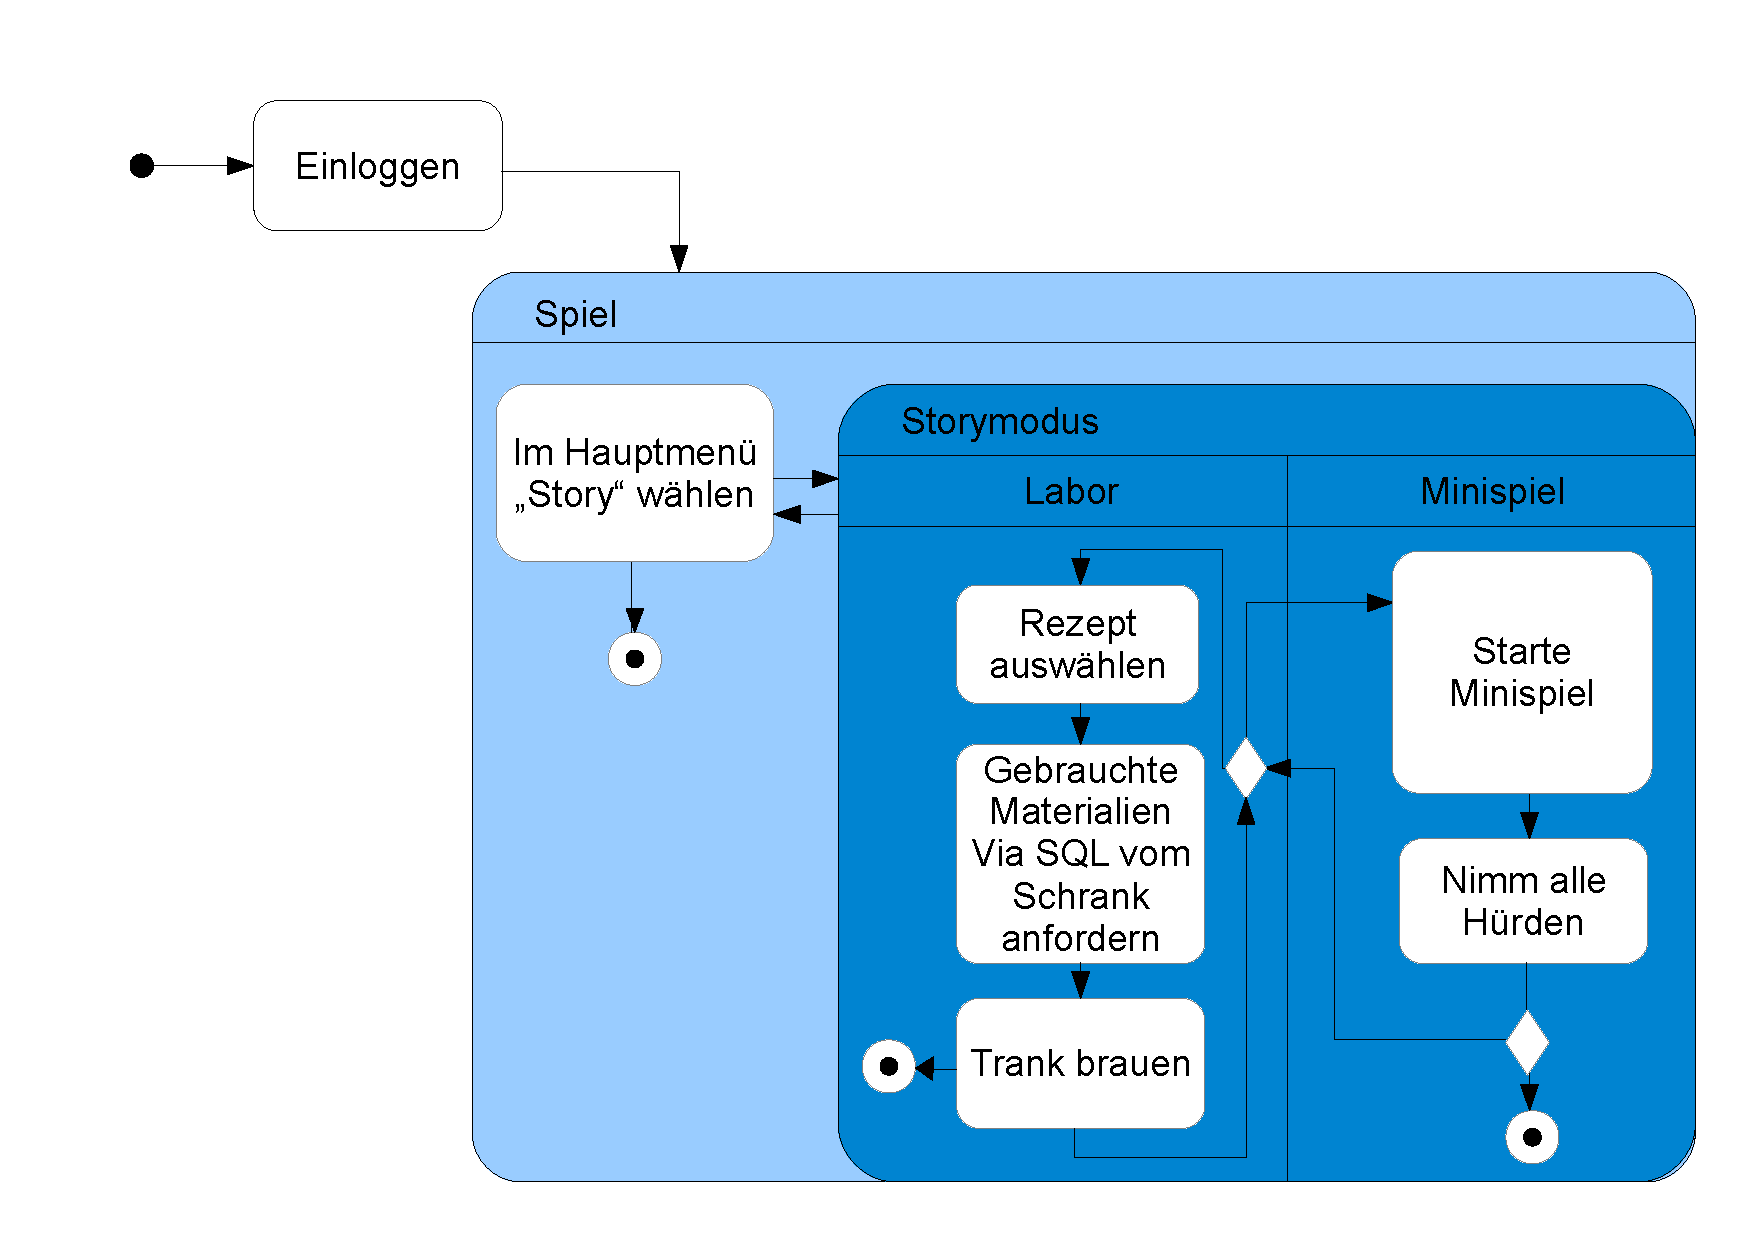
\includegraphics[width=0.9\textwidth]{figures/Aktivitaetsdiagramm.pdf}
\caption{Aktivitätsdiagramm für den Story Mode}
\label{sequence_f120}
\end{figure}
Der Story-Mode besteht zu sich abwechselnden Teilen aus SQL-Trainer und Minispiel. Um dies  besser zu zeigen, ist in Abbildung \ref{sequence_f120} das Aktivitätsdiagramm für den Story Mode aus dem Pflichtenheft abgebildet.\\
Darin ist zu sehen, dass man sich im Labor einen oder mehrere Tränke brauen kann (SQL-Trainer-Anteil), um diese dann im Dungeon zu verwenden (Minispiel-Anteil).
Um die beiden Teile für sich besser beschreiben zu können, sind diese in den folgenden zwei Funktionen separat aufgeführt.
%==================================================================

\newpage
\section{Analyse von Funktionalität <F130>: <SQL-Trainer spielen>}
\begin{figure}[h]
\centering
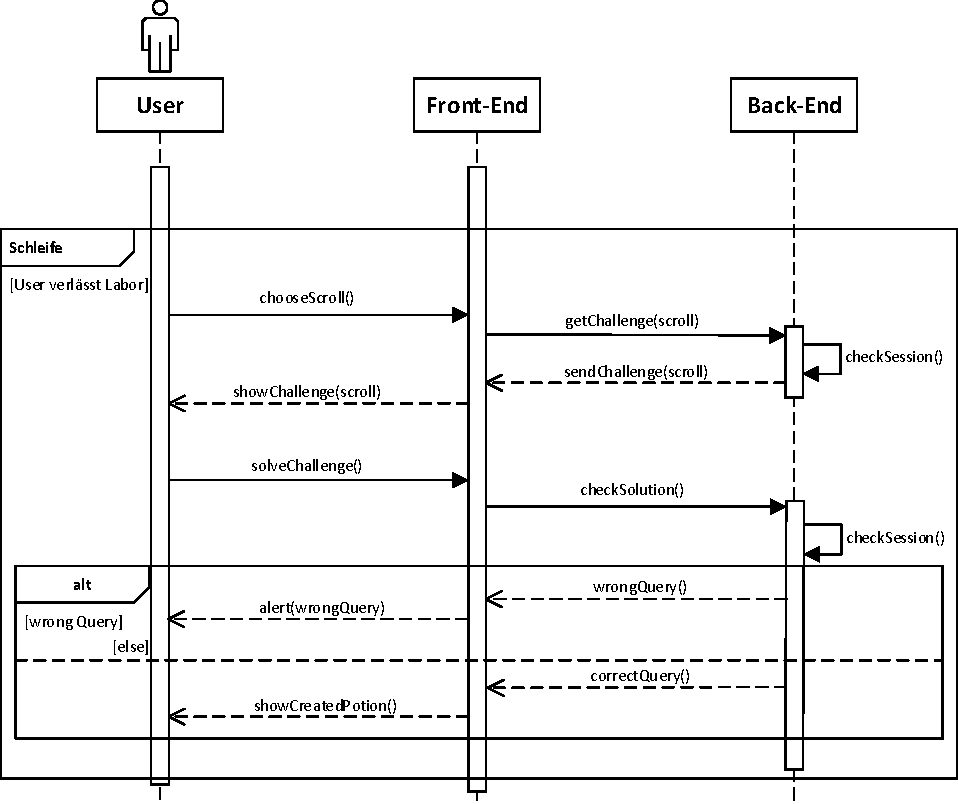
\includegraphics[width=0.9\textwidth]{figures/sequenz_F130.pdf}
\caption{Sequenzdiagramm für den SQL-Trainer}
\label{sequence_f130}
\end{figure}

Der SQL-Trainer ist Teil der drei Spielmodi (Story, Trivia, Homework) und wird einmal (wie er im Trivia-Mode verwendet wird) erklärt. Die leichten Abweichungen der anderen Spielmodi werden im Anschluss erwähnt. Diese benötigen wenig bis gar keine weitere Erklärung, da sie nur einen oberflächlichen Unterschied machen.
Zuerst werden dem User f\"unf Schwierigkeitsgrade angezeigt, aus denen er wählen kann. Hat er sich für einen Schwierigkeitsgrad entschieden, wird dies dem Back-End mitgeteilt, welches daraufhin eine, dem gewählten Schwierigkeitsgrad entsprechende, Aufgabe bereitstellt. Diese kann dann vom User gelöst werden. Die Eingaben werden dabei immer an das Back-End geschickt und dort auf Richtigkeit geprüft. 
Ist die Prüfung positiv verlaufen, wird der User wieder zur Schwierigkeitsgrad-Auswahl weitergeleitet.\\
\newpage
Abweichungen zum Story-Mode:\\
Es werden keine Schwierigkeitsgrade angezeigt, sondern schon eingesammelte Rezepte für Tränke. Diese beinhalten in ihrer Definition schon die Schwierigkeitsgrade für die daraus hervorgehenden Aufgaben.


Abweichungen zum Homework-Mode:\\
Beim Homework-Mode wird die Auswahl des Schwierigkeitsgrades in jeglicher Form übersprungen und der Aufgabentext wird direkt angezeigt.  
%==================================================================

\newpage
\section{Analyse von Funktionalität <F140>: <Minispiel spielen>}
\begin{figure}[h]
\centering
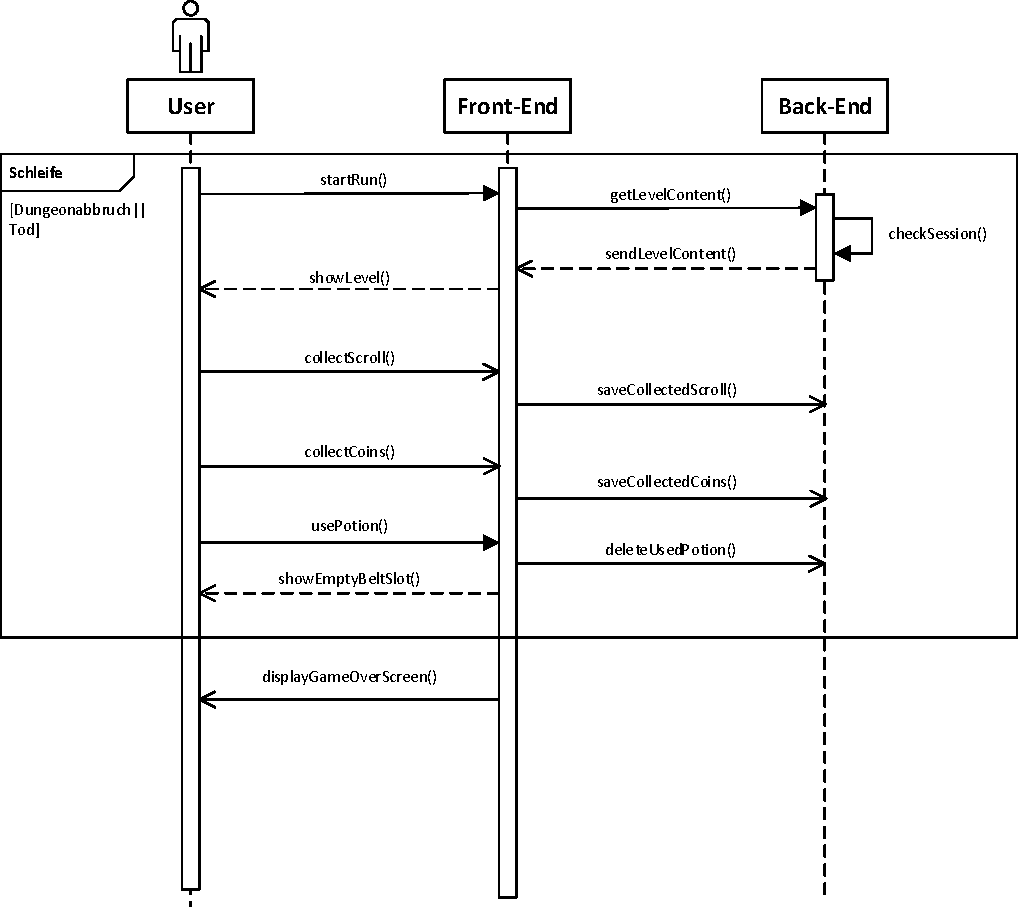
\includegraphics[width=0.9\textwidth]{figures/sequenz_F140.pdf}
\caption{Sequenzdiagramm für das Minigame}
\label{sequence_f140}
\end{figure}
Die Abbildung \ref{sequence_f140} zeigt die Abläufe im Dungeon.

Im Minispiel bewegt sich die Figur stetig nach rechts. Der User kann springen, wodurch er verschiedene Hindernisse überwinden kann. Des Weiteren kann der User Lofi-Coins und Scrolls einsammeln. Dies wird sofort im Back-End vermerkt und im Spielerprofil und im Storyprogress gespeichert. Dem User ist zudem möglich, vorher erstellte Potions zu verwenden, um deren Effekte zur Überwindung von Hindernissen zu nutzen.

%==================================================================

\section{Analyse von Funktionalität <F150>: <Hausaufgaben bearbeiten>}
Die Bearbeitung von Hausaufgaben funktioniert wie das Nutzen des SQL-Trainers. Genauere Erklärungen sind unter (F130) zu finden. Von der dortigen Beschreibung gibt es allerdings folgende Abweichungen: 

Bei den Hausaufgaben handelt es sich um Aufgabenpakete, welche durch die Lehrenden des Moduls RDB1 erstellt werden und den Studenten, die das Modul belegen, zugewiesen werden. Alle anderen Nutzer der Anwendung haben keinen Zugriff auf diese Aufgaben. Die gestellten Aufgabenpakete werden dann als Teil der Studienleistung betrachtet, welche erfüllt werden muss, um RDB1 zu bestehen. Daher sind die Aufgaben nur in den vorgesehenen Bearbeitungszeiträumen erreichbar und zur Bearbeitung freigegeben. 
%==================================================================

\section{Analyse von Funktionalität <F160>: <Ranglisten einsehen>}
\begin{figure}[h]
\centering
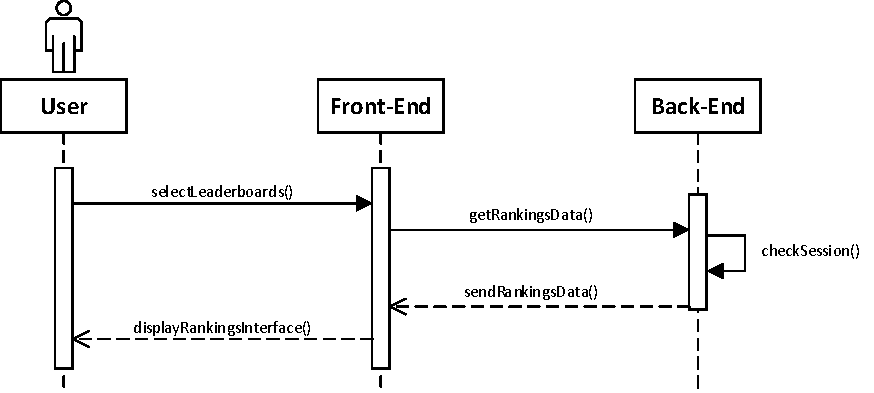
\includegraphics[width=0.9\textwidth]{figures/sequenz_F160.pdf}
\caption{Sequenzdiagramm für die Ranglisten}
\label{sequence_f160}
\end{figure}
In Abbildung \ref{sequence_f160} wir das Anzeigen der Ranglisten dargestellt.

Möchte der User die Ranglisten einsehen, wird eine Anfrage an das Back-End gesendet. Das Back-End stellt dann die Daten für die Ranglisten zusammen und sendet diese zurück an das Front-End, wo diese dann für den User einsehbar präsentiert werden.
%==================================================================

\newpage
\section{Analyse von Funktionalität <F170>: <Spieler suchen>}
\begin{figure}[h]
\centering
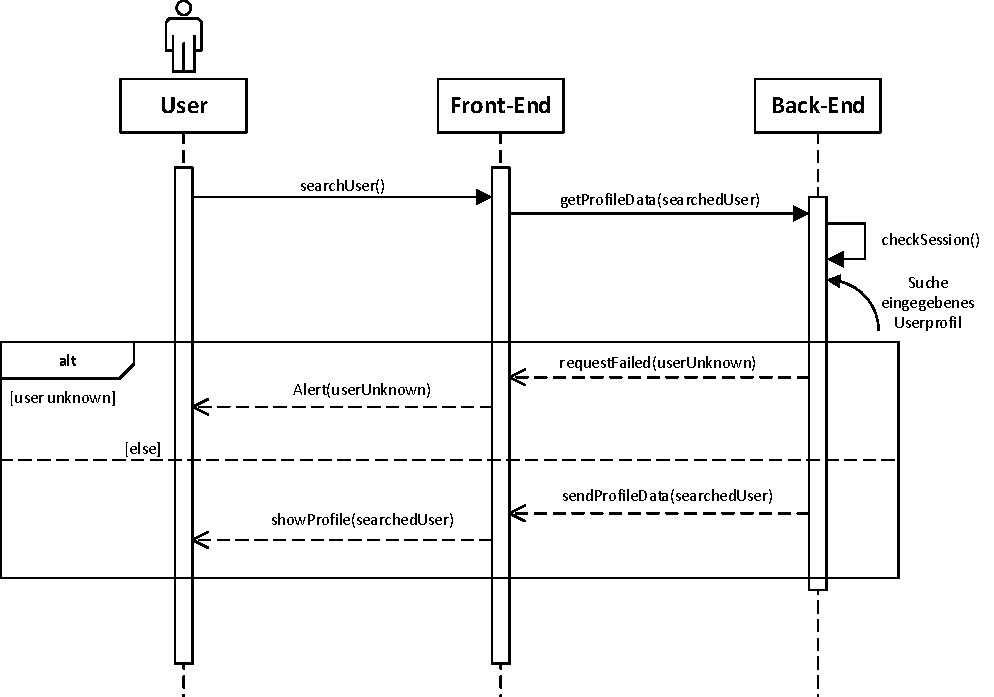
\includegraphics[width=0.9\textwidth]{figures/sequenz_F170.pdf}
\caption{Sequenzdiagramm zum Suchen eines anderen Users}
\label{sequence_f170}
\end{figure}
Im Diagramm \ref{sequence_f170} ist zu sehen, wie man nach einem anderen User suchen kann.

Um einen anderen User zu suchen, wird ein Eingabefeld bereitgestellt. Der dort eingegebene Name wird an das Back-End weitergeleitet, dort in der Userdatenbank gesucht und wenn er existiert, wird dessen Profil aus der Datenbank geladen und dem suchenden User angezeigt. Ist der Name in der Datenbank nicht zu finden, wird dies dem suchenden User mitgeteilt.

Der Zweck der Suche ist es, dass die User die Profile anderer Spieler einsehen können, um sich mit diesen vergleichen zu können. Dies kann aus Gründen des Wettbewerbs untereinander oder einfach aus dem Interesse am Fortschritt von bekannten Usern geschehen. Somit bietet die Funktion den Usern eine simple Möglichkeit sich mit anderen Spielern zu vergleichen.
%================================================================== 

\newpage
\section{Analyse von Funktionalität <F180>: <Hausaufgabenergebnisse einsehen>}
\begin{figure}[h]
\centering
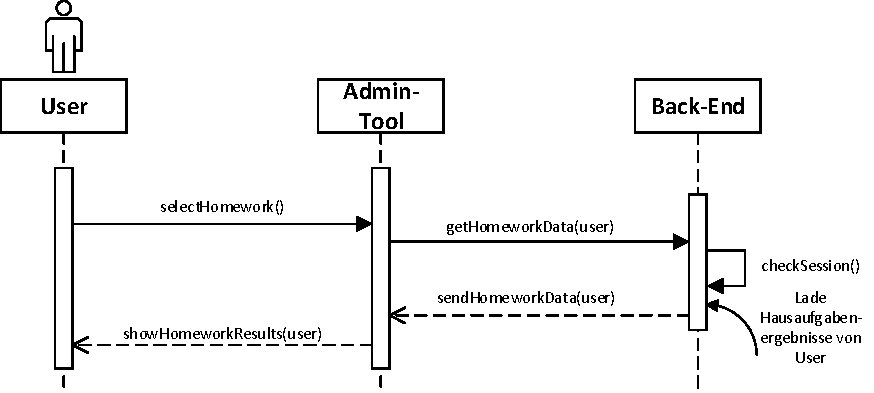
\includegraphics[width=0.9\textwidth]{figures/sequenz_F180.pdf}
\caption{Sequenzdiagramm zum einsehen der eigenen Hausaufgabenergebnisse}
\label{sequence_f180}
\end{figure}
Abbildung \ref{sequence_f180} beschreibt das Anzeigen der Hausaufgabenergebnisse.

Nach dem Einloggen in das Admintool werden die Hausaufgabenergebnisse eines nicht-beförderten Users direkt aus der Datenbank geladen und angezeigt.
Ist der User schon \glqq befördert\grqq , muss er erst noch auf den \glqq Show Homework Results \grqq -Button drücken.
%==================================================================

\newpage
\section{Analyse von Funktionalität <F190>: <Benutzer befördern>}
\begin{figure}[h]
\centering
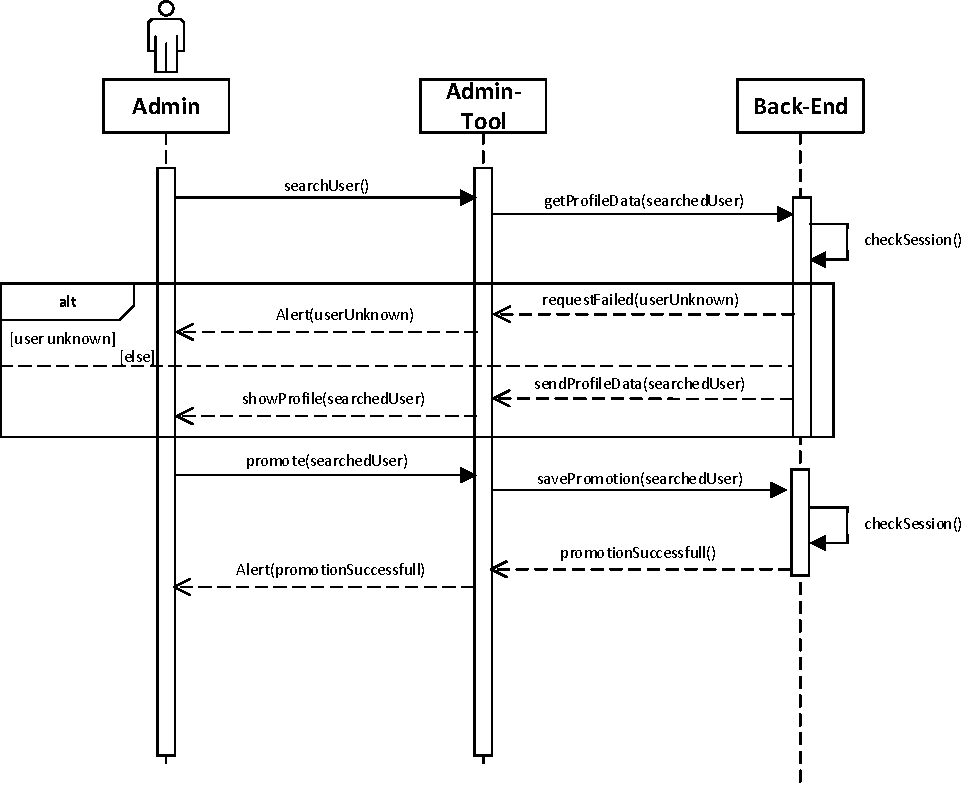
\includegraphics[width=0.9\textwidth]{figures/sequenz_F190.pdf}
\caption{Sequenzdiagramm zum Befördern eines Users}
\label{sequence_f190}
\end{figure}
Abbildung \ref{sequence_f190} beschreibt das Befördern eines Benutzers.

Zuerst wird für den Admin die Userdatenbank angezeigt. Hier kann er entweder manuell oder per Suchfunktion nach einem User suchen und diesen per Knopfdruck befördern, was dann im Back-End in den jeweiligen Userdaten registriert und gespeichert wird. 

Der Ablauf, einem User Adminrechte (<F200>) zu geben, gleicht dem des User Bef\"orderns.
%==================================================================

\newpage
\section{Analyse von Funktionalität <F210>: <Eine Trivia-Aufgabe erstellen>}
\begin{figure}[h]
\centering
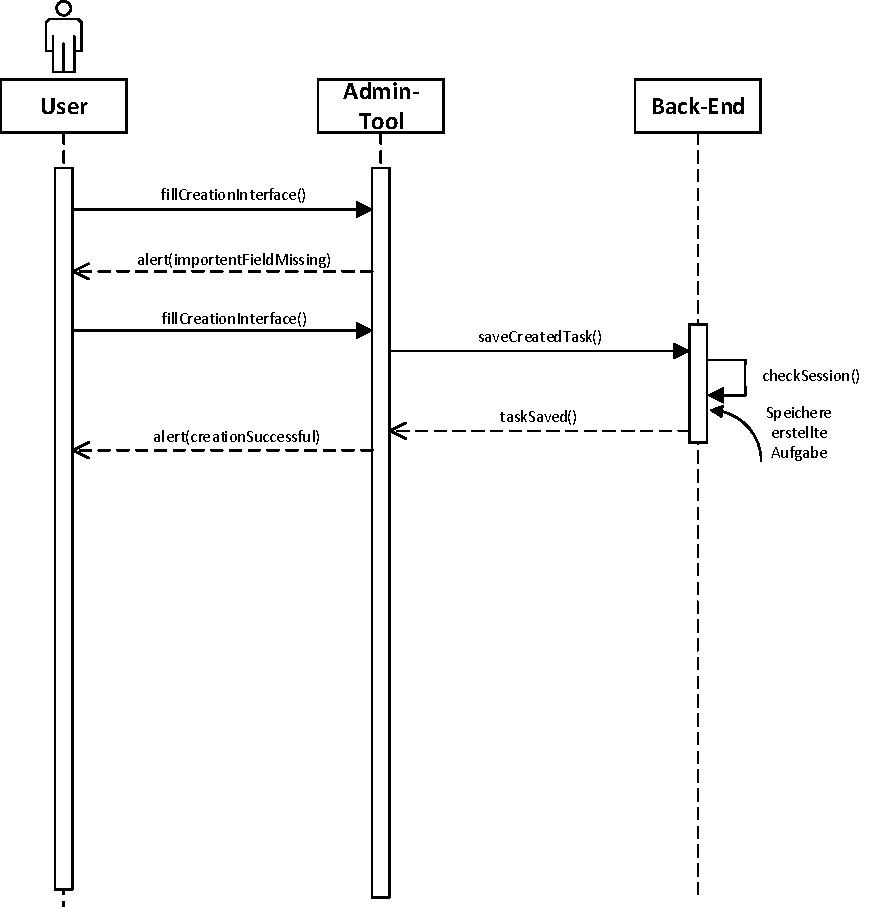
\includegraphics[width=0.9\textwidth]{figures/sequenz_F210.pdf}
\caption{Sequenzdiagramm für das Erstellen von Aufgaben}
\label{sequence_f210}
\end{figure}
Abbildung \ref{sequence_f210} beschreibt das Erstellen von eigenen Aufgaben.

Beförderte Nutzer können selber Aufgaben erstellen, welche später im Trivia Mode verwendet werden können.
Dafür steht im Admin-Tool ein Interface zur Verfügung, in das ganz einfach alle zur Aufgabe gehörigen Daten eingetragen und dann an das Back-End gesendet werden, wo die Aufgabe gespeichert wird. Sind nicht alle wichtigen Felder ausgefüllt, wird der User alarmiert und muss dies berichtigen, damit die Aufgabe abgespeichert werden kann.
%==================================================================

\newpage
\section{Analyse von Funktionalität <F220>: <Benutzeraufgaben bewerten>}
\begin{figure}[h]
\centering
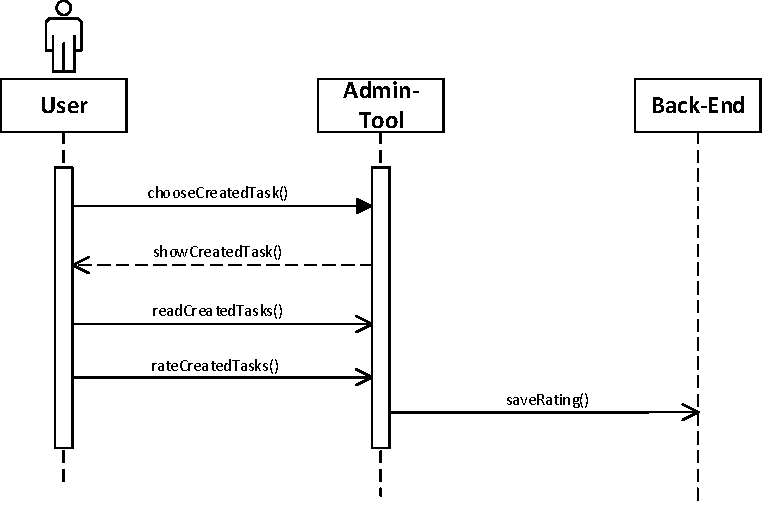
\includegraphics[width=0.9
\textwidth]{figures/sequenz_F220.pdf}
\caption{Sequenzdiagramm zum bewerten User-erstellter Aufgaben.}
\label{sequence_f220}
\end{figure}
Abbildung \ref{sequence_f220} zeigt den Ablauf, wie man eine von Usern erstellte Aufgabe bewertet.

In der Liste aller von Usern erstellten Aufgaben kann sich der User Aufgaben aussuchen, diese ansehen, sie bewerten und kommentieren. Die Bewertung wird dann im Back-End für die Aufgabe registriert und gespeichert. 
%==================================================================

\newpage
\section{Analyse von Funktionalität <F230>: <Hausaufgaben erstellen>}

Die Erstellung von Hausaufgaben gleicht der userseitigen Erstellung von Aufgaben, ist jedoch nur Administratoren zugänglich.

Der Unterschied zur normalen Aufgabenerstellung besteht darin, dass ein Aufgabenpaket erstellt wird. Dabei kann man entweder Aufgaben für das Paket neu erstellen, oder auf schon einmal erstellte Aufgaben, die in der Datenbank gespeichert sind, zugreifen. Diese Aufgabenpakete können dann noch mit zusätzlichen Parametern versehen werden, wie zum Beispiel einem Bearbeitungszeitraum oder einer Anzahl an Versuchen. 

%!TEX root = ../Systementwurf.tex

\chapter{Resultierende Softwarearchitektur}\label{chap:architektur}

Die \NewsGenie Systemarchitektur ist eine klassische Client-Server Architektur, wobei es sich um einen Thin-Client
und einen Fat-Server handelt. Sämtliche Rechenaufwändige Operationen werden dementsprechend auf dem \textit{Server} ausgeführt,
während der \textit{Client} die sprachbasierte Bedienung durch den User umsetzt. Allerdings werden kleinere und ressourcenarme  Sprachverarbeitungsdienste zum Zweck einer zeitlichen Performancesteigerung ebenfalls am \textit{Client}
realisiert. Diese beinhalten die Verarbeitung von Anfragen der einfachsten Art, in erster Linie einfache Navigationsbefehle, wie das Auswählen eines von mehreren vorgeschlagenen Nachrichtenartikeln. 
Die Kommunikation mit der \textit{Google-Speech-API} findet ebenfalls auf dem \textit{Client} statt.

Die Architektur des \textit{Servers} ist in vier Komponenten geteilt. Das Kernelement für die Datenspeicherung ist 
die mit Triplen realisierte \textit{Datenbank} und der \textit{Crawler}, welcher permanent die ausgewählten Nachrichtenseiten nach neuen Artikeln durchsucht, um diese dann speichern zu lassen. Aus der vom \textit{Client} empfangenen Useranfrage und den vorhandenen Artikeln in der \textit{Datenbank} eine relevante Antwort zu generieren ist Aufgabe des \textit{Query Processors}. 
Der \textit{Server} bietet darüber hinaus ein \textit{Web Interface} an, welches es dem User oder Administrator ermöglicht Benutzereinstellungen zu verändern.

Die Architektur des \textit{Query Processors} unterteilt sich in sechs weitere Komponenten. Herzstück ist der \textit{Query Handler}.
Diese Komponente steuert den Ablauf des \textit{Query Processors} und regelt das Zusammenspiel der anderen Komponenten. 
Die erste anzusteuernde Komponente ist \textit{Natural Language Processing}, welches die Satzstruktur der Useranfrage analysiert. Darauf aufbauend ist es im \textit{Analyzer} möglich die Intention der Nutzeranfrage zu bestimmen, wie z.B. Neuigkeiten im Bereich der Technologie zu finden, oder Informationen zu einer bestimmten Person zu nennen. 
Der \textit{Searcher} kann dementsprechend agieren und eine geeignete Anfrage an die Datenbank stellen. Im Falle einer Entitätsfrage, wie das erwähnte Fragen nach dem Alter einer Person, wird die \textit{Linked Open Data}-Komponente angesteuert, andernfalls die \textit{Datenbank}.
Die Informationen der Linked Open Data können durch die \textit{Linked Open Data} Komponente schnell und effizient abgefragt werden, um dementsprechende faktuale Anfragen beantworten zu können. 
Die bis hierhin entstandenen Ergebnisse des Prozesses werden daraufhin an die \textit{Result Processing} Komponente übermittelt.
Aufgabe dieser ist es, die Ergebnisse für die Sprachausgabe am \textit{Client} vorzubereiten, also den Ausgabestring zu generieren. Dazu zählt auch die Aufgabe durch Textbausteine für eine natürlich klingende und abwechslungsreiche Sprache zu sorgen.

\section{Komponentenspezifikation}

%In diesem Abschnitt wird die aus der Analyse der Produktfunktionen (\autoref{chap:analyse}) resultierende Komponentenstruktur zunächst überblickartig durch ein Komponentendiagramm beschrieben. Die Bezeichnungen und Anzahl der Komponenten
%muss natürlich konsistent sein mit der in \autoref{chap:analyse}!

%Die einzelnen Komponenten werden anschließend kurz beschrieben.

Die aus Abschnitt \ref{chap:analyse} resultierende Komponentenarchitektur ist in Abb.~\ref{fig:Komponenten} in Form eines Komponentendiagramms abgebildet. Die Komponente \textit{Query Processor} wird außerdem in Abb.~\ref{fig:Komponenten_QP} in ihre Unterkomponenten aufgeschlüsselt.

\begin{figure}
\centering
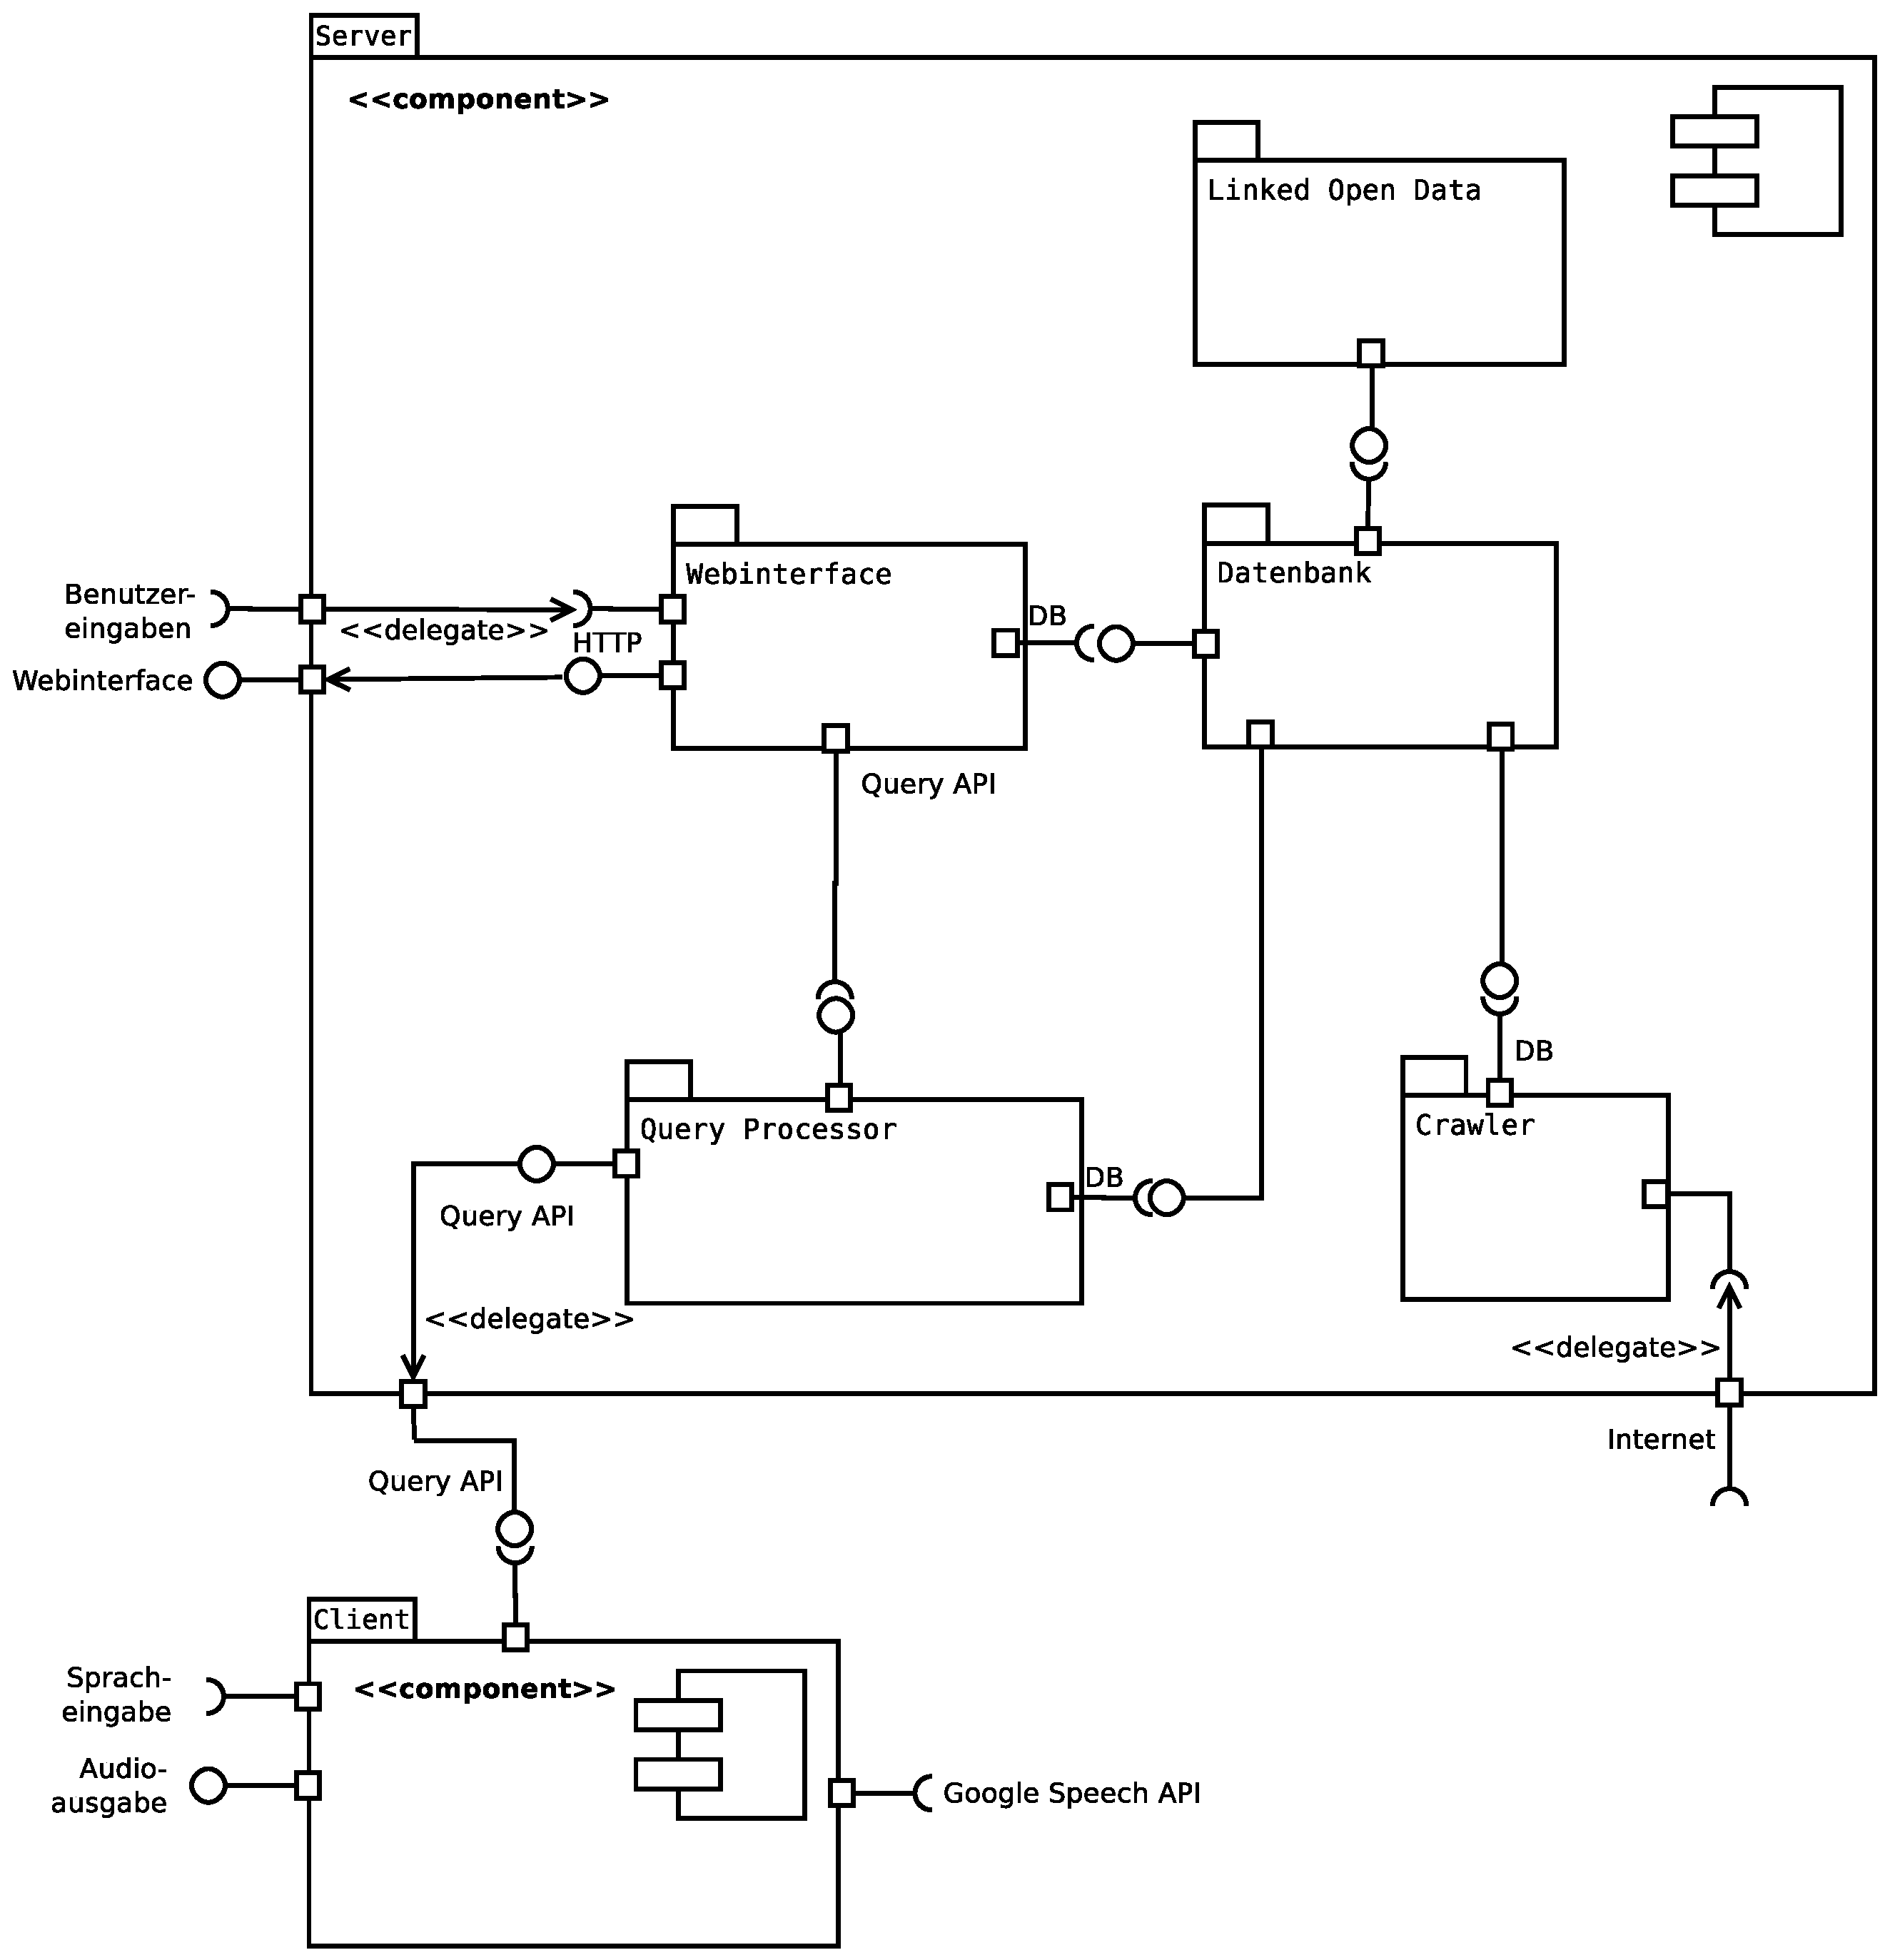
\includegraphics[width=1\linewidth]{Systementwurf/05_implementierungsentwurf/komponenten}
\caption{\textit{\NewsGenie Komponentendiagramm}}
\label{fig:Komponenten}
\end{figure}

\begin{figure}
\centering
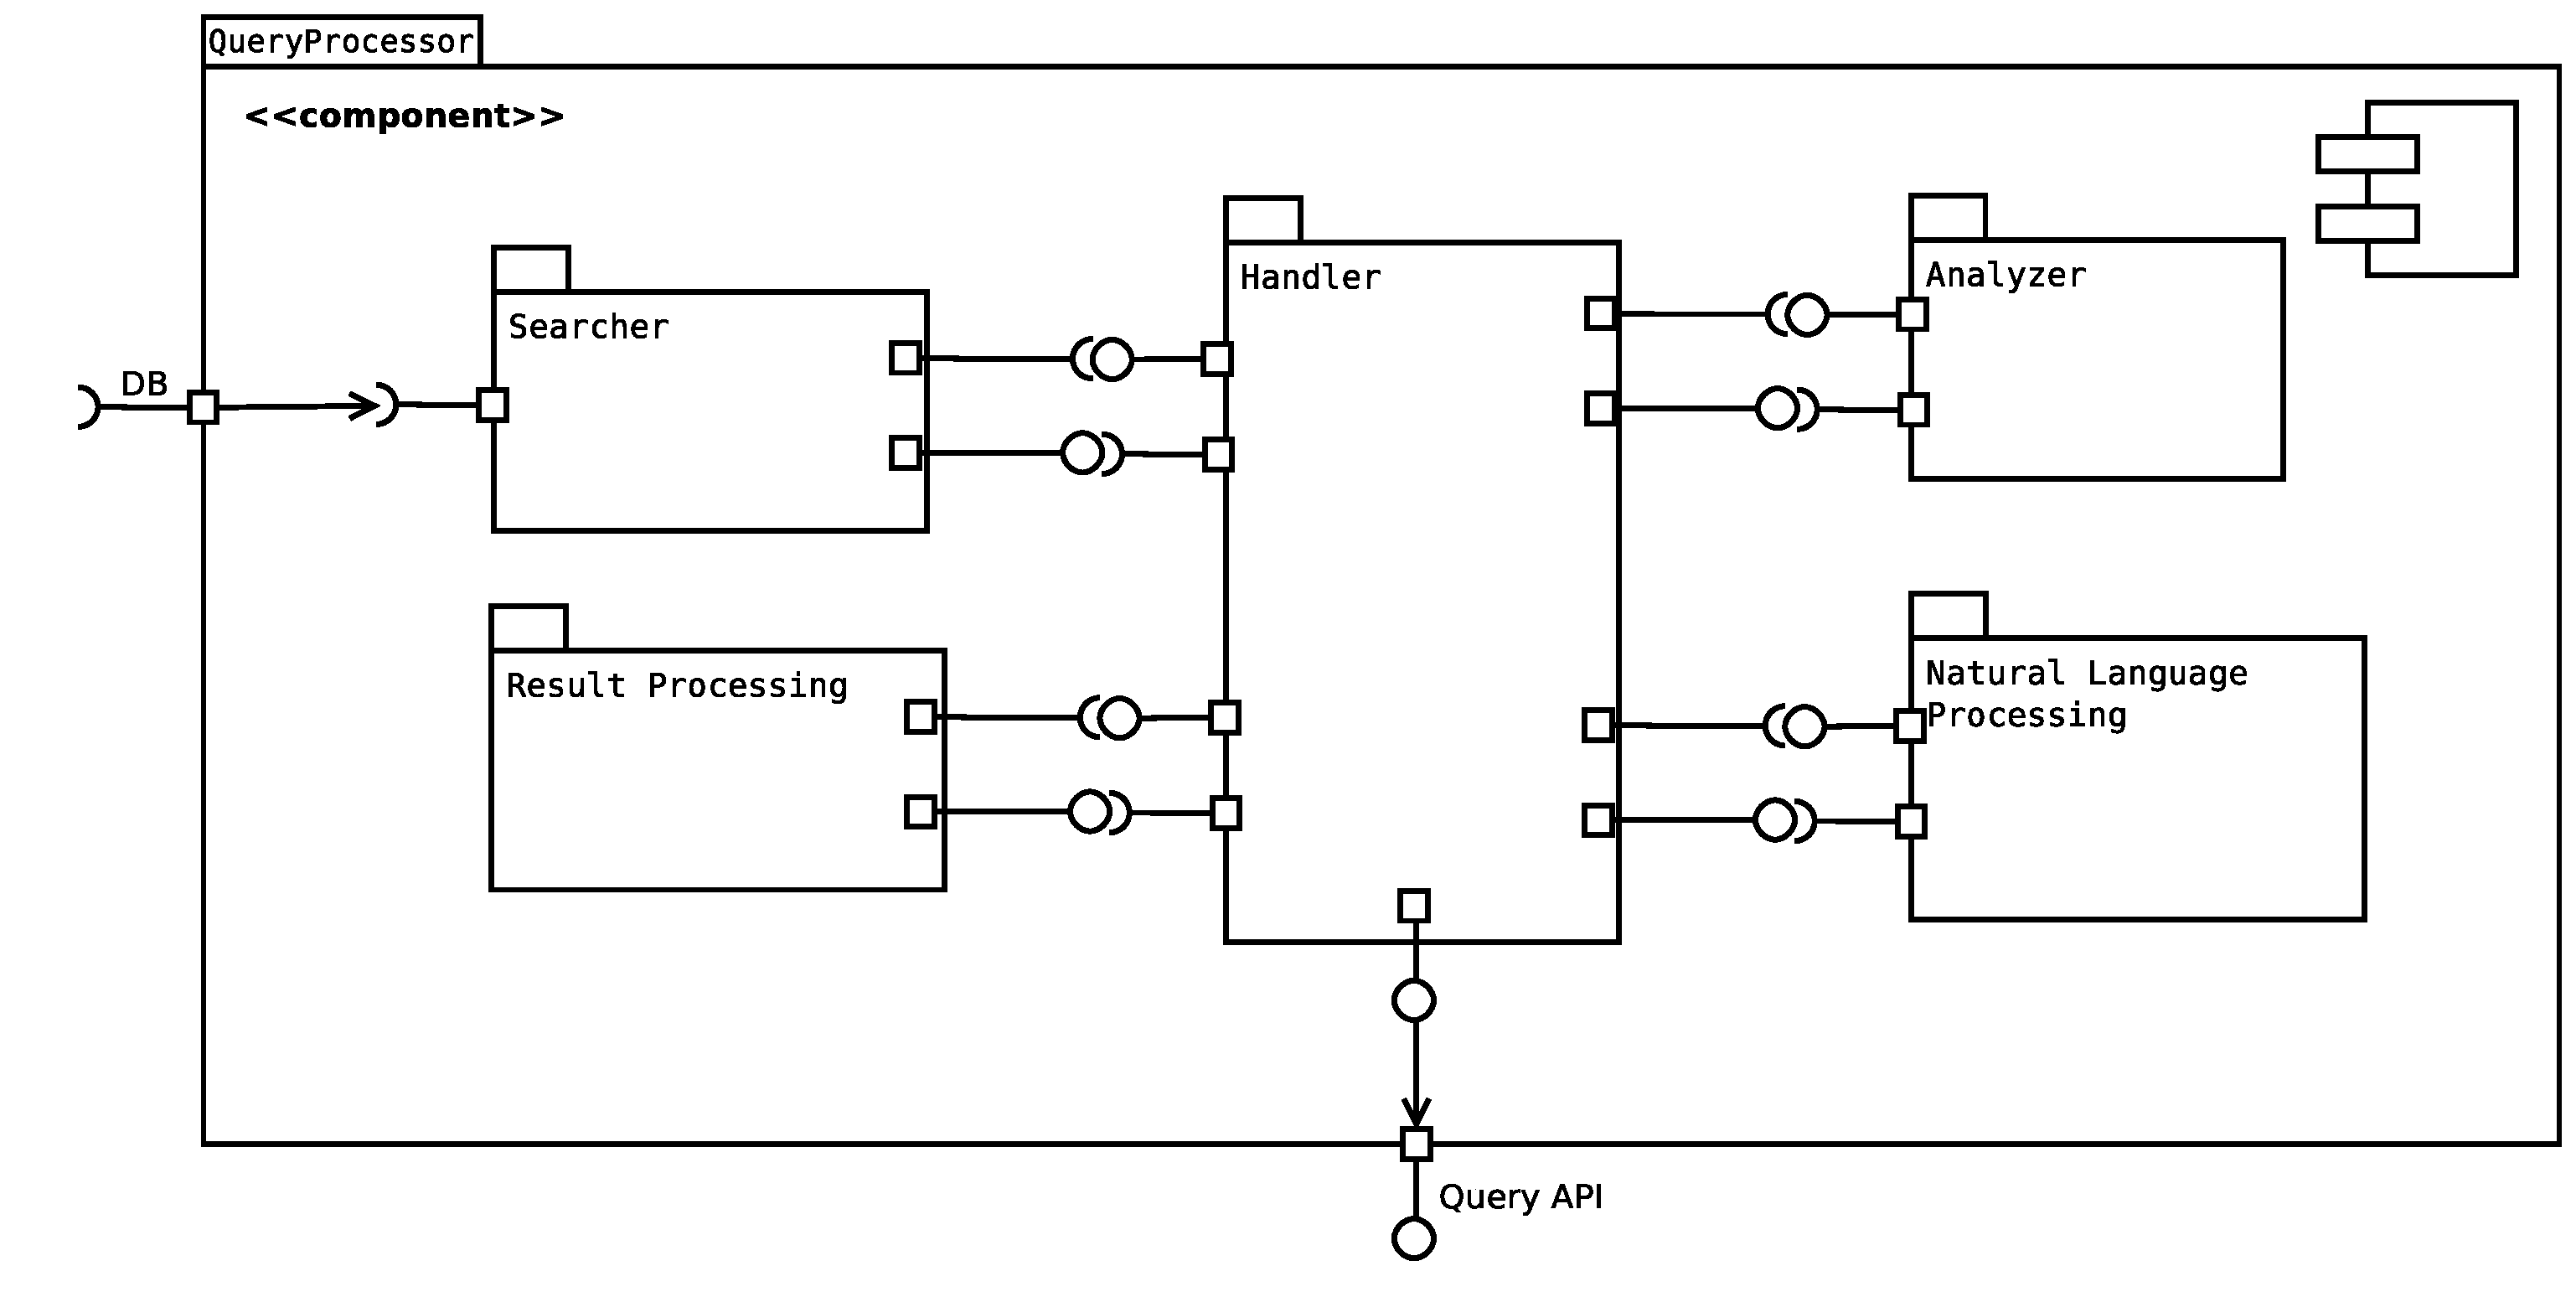
\includegraphics[width=1\textheight, angle=90]{Systementwurf/05_implementierungsentwurf/paket-queryprocessor}
\caption{\textit{\NewsGenie Komponentendiagramm - Query Processor}}
\label{fig:Komponenten_QP}
\end{figure}

\begin{component}{10}{Client}
Auf dem \textit{Client} werden die Hauptfunktionen der Sprach Ein- und Ausgabe realisiert. Der \textit{Client} ist somit die Hauptschnittstelle des Benutzers. Der Zugriff auf die \textit{Google Speech API} wird auf dem \textit{Client} realisiert. 
Die Komponente ist zusätzlich dazu in der Lage, auf simple Navigationsbefehle zu reagieren, ohne den \textit{Server} 
kontaktieren zu müssen.
\end{component}

\begin{component}{20}{Webinterface}
Das \textit{Web Interface} ist die zweite Schnittstelle für den Benutzer. Es stellt Konfigurations- und 
Administrationsfunktionen zur Verfügung, wie Nutzerregistrierung, Passwortmanagement, das Abonnement-Management
der Nachrichtenfeeds oder auch das Löschen von Nutzern.
\end{component}

\begin{component}{30}{Datenbank}
Realisiert die Speicherung der relevanten Daten über die User und die Nachrichtenartikel.
Die Speicherstruktur ist mit Tripeln implementiert.
\end{component}

\begin{component}{35}{Linked Open Data}
Komponente für den Zugriff auf die Linked Open Data. Sie liefert Informationen zu bestimmten
Entitätsfragen nach Personen oder Orten.
\end{component}

\begin{component}{40}{Crawler}
Der \textit{Crawler} liefert die Daten für die \textit{Datenbank}, indem er das Internet nach Nachrichtenartikeln
durchsucht, welche anschliessend gespeichert werden.
\end{component}

\begin{component}{50}{Query Processor}
Der \textit{Query Processor} verarbeitet die am \textit{Client}/\textit{Web Interface} gestellten Anfragen um die Intention
des Users zu erkennen und dementsprechend Anfragen an die \textit{Datenbank} zu stellen. Die Ergebnisse
werden an den \textit{Client} zurück gegeben.
Die Komponente besteht aus den Unterkomponenten \textit{Handler}, \textit{Natural Language Processing}, \textit{Analyzer}, \textit{Searcher}, \textit{Linked Open Data}, und \textit{Result-Processing}.
\end{component}

\begin{component}{60}{Handler}
Der \textit{Handler} steuert durch Aufrufe der anderen Komponenten den Ablauf im Query Processor. Sie ist die Komponente die von aussen angesteuert wird. 
\end{component}

\begin{component}{70}{Natural Language Processing}
Die als String eingehenden Anfragen werden auf ihre Satzstruktur analysiert. Es werden Subjekt, Objekt und Prädikat erkannt.
Darüber hinaus wird der Satz als Baumstruktur abgespeichert, was es ermöglicht Nebensätze und Hauptsätze zu erkennen. 
\end{component}

\begin{component}{80}{Analyzer}
Aufbauend auf \textit{Natural Language Processing} kann die Anfrage in dieser Komponente tiefer gehend analysiert werden. Sie bestimmt den Fragetyp, d.h. Entitätsfrage oder Nachrichtenanfrage, und kann somit die Intention des Users analysieren. 
\end{component}

\begin{component}{90}{Searcher}
Aufbauend auf den \textit{Analyzer} kann der \textit{Searcher} Datenbankanfragen stellen, um die passenden Ergebnisse zu bekommen.
Bei Entitätsfragen wird \textit{Linked Open Data} angesteuert, welche mit Daten aus der Linked Open Data antworten kann. 
\end{component}

\begin{component}{100}{Result Processing}
Im \textit{Result Processing} werden die Ergebnisse als String aufbereitet. Dabei werden variable Textbausteine verwendet um eine möglichst natürliche und flüssige Sprachausgabe zu gewährleisten.
\end{component}


\section{Schnittstellenspezifikation}

%Im Folgenden werden die einzelnen Schnittstellen der Komponenten aus der
%Komponentenspezifikation näher erläutert, d.h. die von Ihnen zur Verfügung
%gestellten Operationen werden dokumentiert. Die Tabelle ist dabei um so viele
%Zeilen zu erweitern, wie es Schnittstellen im Komponentendiagramm gibt. In der
%innen liegenden Aufteilung ist für jede Operation einer Schnittstelle eine
%Zeile einzufügen.  Reine Set- und Get-Aufrufe brauchen nicht aufgeführt zu
%werden (sollten auch möglichst nicht komponentenübergreifend auftauchen).

\textbf{Hinweis:}
Durch die Verwendung des Akka-Frameworks für die Komponenteninteraktion zwischen
Client, Server, Datenbank, Crawler und Webinterface werden, statt einzelne
Nachrichten, Objekte verschickt.
Daher sind bei Kommunikationen zwischen diesen Komponenten die Operationen als
ins Netzwerk angebotene Objekte zu betrachten.
Alle anderen Komponentenkommunikationen sind als Funktionsaufrufe aus den fünf
oben genannten Komponenten zu sehen.

\begin{interface}{10}{Client Schnittstelle}
\begin{tabular}[ht]{|p{5cm}|p{9cm}|}
\hline
Operation & Beschreibung\\
\hline
ClientQuery()  & Der Client sendet die Suchanfrage an den Handler,
welcher die Verarbeitung koordiniert.\\
\hline
\end{tabular}
\end{interface}

\begin{interface}{20}{Webinterface Schnittstelle}
\begin{tabular}{|p{5cm}|p{9cm}|}
\hline
Operation & Beschreibung\\
\hline
ClientQuery() & Das Webinterface sendet die Suchanfrage an den Handler,
welcher die Verarbeitung koordiniert.\\
\hline
RegisterRequest() & Die Anfrage einer Registrierung an den Server\\
\hline
WebLoginRequest() & Die Anfrage eines Logins an den Server\\
\hline
UserFeedsRequest() & Die Anfrage, die abbonierten Feeds eines Nutzers zu
bekommen.\\
\hline
AddFeedRequest() & Die Anfrage, einen Feed zu den abbonierten Feeds hinzuzufügen\\
\hline
RemoveFeedRequest() & Die Anfrage, einen Feed von den abbonierten Feeds zu
löschen\\
\hline
ChangePasswordRequest() & Die Anfrage, das Passwort zu ändern\\
\hline
RecoverPasswordRequest() & Die Anfrage, das Passwort wiederherzustellen\\
\hline
UserListRequest() & Die Anfrage, alle Nutzer zu bekommen\\
\hline
DeleteUserRequest() & Die Anfrage, einen User zu löschen\\
\hline
ClientQuery() & Eine Anfrage an das System stellen\\
\hline
\end{tabular}
\end{interface}

\begin{interface}{30}{Datenbank Schnittstelle}
\setlength{\LTpre}{-0,45cm}
\begin{longtable}[l]{|p{5cm}|p{9cm}|}

\hline
Operation & Beschreibung\\
\hline
SearchAnswer() & Die SearchAnswer wird zurück an den Searcher geschickt und
beinhaltet die Suchantwort\\
\hline
ClientLoginAnswer() & Die CLientLoginAnswer wird zurück an den Client geschickt
und beinhaltet den Status, ob der User seine Logindaten korrekt eingegeben hat\\
\hline
RegisterAnswer() & Die RegisterAnswer wird zurück an das Webinterface geschickt
und beinhaltet den Status, ob der User seine Registrierung erfolgreich
abgeschlossen hat\\
\hline
WebLoginAnswer() & Die RegisterAnswer wird zurück an das Webinterface geschickt
und beinhaltet den Status, ob der User seine Logindaten korrekt eingegeben hat\\
\hline
UserFeedsAnswer() & Die UserFeedAnswer wird zurück an das Webinterface geschickt
und beinhaltet eine Liste mit allen abbonierten Feeds des Nutzers\\
\hline
AddFeedAnswer() & Die AddFeedAnswer wird zurück an das Webinterface geschickt
und beinhaltet den Status, ob das Hinzufügen bzw. Löschen eines Feeds für den
Nutzer erfolgreich war\\
\hline
ChangePasswordAnswer() & Die ChangePasswordAnswer wird zurück an das Webinterface geschickt
und beinhaltet den Status, ob das Ändern des Passworts für den
Nutzer erfolgreich war\\
\hline
RecoverPasswordAnswer() & Die RecoverPasswordAnswer wird zurück an das Webinterface geschickt
und beinhaltet den Status, ob das Zurücksetzen des Passworts für den
Nutzer erfolgreich war\\
\hline
UserListAnswer() & Die UserFeedAnswer wird zurück an das Webinterface geschickt
und beinhaltet eine Liste mit allen Nutzern\\
\hline
DeleteUserAnswer() & Die DeleteUserAnswer wird zurück an das Webinterface geschickt
und beinhaltet den Status, ob das Löschen eines Nutzers erfolgreich war\\
\hline
FactAnswer() & Die FactAnswer wird von Linked Open Data zurück an den Searcher
geschickt und beinhaltet die Link Open Data Antwort\\
\hline
UpdateArticleAnswer() & Die UpdateFeedAnswer wird zurück an den Crawler
geschickt und beinhaltet den Status, ob das Hinzufügen erfolgreich war\\
\hline
\end{longtable}
\end{interface}

\begin{interface}{40}{Crawler Schnittstelle}
\begin{tabular}[ht]{|p{4cm}|p{10cm}|}
\hline
Operation & Beschreibung\\
\hline
CrawlerAnswer() & Der Crawler sendet eine Liste von Artikeln, welche von
der Datenbank hinzugefügt werden sollen\\
\hline
\end{tabular}
\end{interface}

\begin{interface}{50}{Query Processor Handler Schnittstelle}
\begin{tabular}[ht]{|p{4cm}|p{10cm}|}
\hline
Operation & Beschreibung\\
\hline
ClientAnswer() & Die ClientAnswer wird zurück an den Managment Handler
geschickt und beinhaltet die Antwort auf die Nutzeranfrage\\
\hline
\end{tabular}
\end{interface}

\begin{interface}{60}{Managment Handler Schnittstelle}
\begin{tabular}[ht]{|p{4cm}|p{10cm}|}
\hline
Operation & Beschreibung\\
\hline
ClientQuery()  & Query Processor bekommt vom Handler die Suchanfrage und
koordiniert die Verarbeitung dieser.\\
\hline
ClientAnswer() & ClientAnswer wird vom QueryProcessor an den Client
weitergeleitet.\\
\hline
\end{tabular}
\end{interface}

\begin{interface}{70}{Natural Language Processing Schnittstelle}
\begin{tabular}[ht]{|p{4cm}|p{10cm}|}
\hline
Operation & Beschreibung\\
\hline
analyse() & Verarbeitet den übergebenen Text und gibt eine Liste der Tokens an
den Query Processor Handler\\
\hline
 \end{tabular}
\end{interface}

\begin{interface}{80}{Analyzer Schnittstelle}
\begin{tabular}[ht]{|p{4cm}|p{10cm}|}
\hline
Operation & Beschreibung\\
\hline
analyse() & Verarbeitet die übergebene Liste von Tokens und gibt alles Nötige
für die Datenbanksuche an den Query Processor Handler\\
\hline
 \end{tabular}
\end{interface}

\begin{interface}{90}{Searcher Schnittstelle}
\begin{tabular}[ht]{|p{4cm}|p{10cm}|}
\hline
Operation & Beschreibung\\
\hline
SearchRequest() & Ein SimpleSearchRequest wird an die Datenbank
geschickt mit allen nötigen Informationen für die Suche\\
\hline
search() & Sucht mithilfe des SimpleSearchRequest in der Datenbank\\
\hline
 \end{tabular}
\end{interface}

\begin{interface}{100}{Result Processing Schnittstelle}
\begin{tabular}[ht]{|p{4cm}|p{10cm}|}
\hline
Operation & Beschreibung\\
\hline
makeClientAnswer() & Eine ClientAnswer wird erstellt und an den Query Processor
Handler zurückgegeben\\
\hline
 \end{tabular}
\end{interface}

\begin{interface}{110}{Linked Open Data Schnittstelle}
\begin{tabular}[ht]{|p{4cm}|p{10cm}|}
\hline
Operation & Beschreibung\\
\hline
searchfor() & Eine FactAnswer wird erstellt und an die Datenbank zurückgegeben\\
\hline
 \end{tabular}
\end{interface}



\section{Protokolle für die Benutzung der Komponenten}

Speziell der \textit{Client} ist auch in anderen Projekten sinnvoll nutzbar.
Er realisiert eine Komponente mit sprachbasiertem In- und Output, welche auch in einem gänzlich anderen Kontext genutzt werden kann.
Der \textit{Server} dagegen erfordert lediglich eine User Input-Komponente, wie z.B. den \textit{Client} um zu funktionieren. 
Ein alternatives Szenario wäre somit nur der Austausch der Nutzerschnittstelle, wobei die Kernfunktionen des Projektes gleich blieben.
Es ist allerdings denkbar, Unterkomponenten des \textit{Servers} in anderen Zusammenhängen zu verwenden.
Das Web-Crawling nach News durch den \textit{Crawler} ließe sich z.B. auch in anderen Projekten verwenden.
Der \textit{Query Processor} ist zu stark spezialisiert auf das gegebene Aufgabenfeld als dass er wirklich sinnvoll generisch in anderen Projekten genutzt werden könnte. Die Unterkomponenten \textit{Natural Language Processing} und \textit{Linked Open Data} könnten
theoretisch in andere Bereiche übernommen werden, es würde sich aber auf Grund des geringen Programmieraufwandes kaum lohnen.
Solche Klassen würde man spezialisiert auf das entsprechende Aufgabenfeld eines Projektes neu schreiben.

Der \textit{Client} und der \textit{Crawler} funktionieren als eigenständige Subsysteme und sind in Abb.~\ref{fig:client_chart} und Abb.~\ref{fig:crawler_chart} als Statecharts abgebildet.

\begin{figure}
\centering
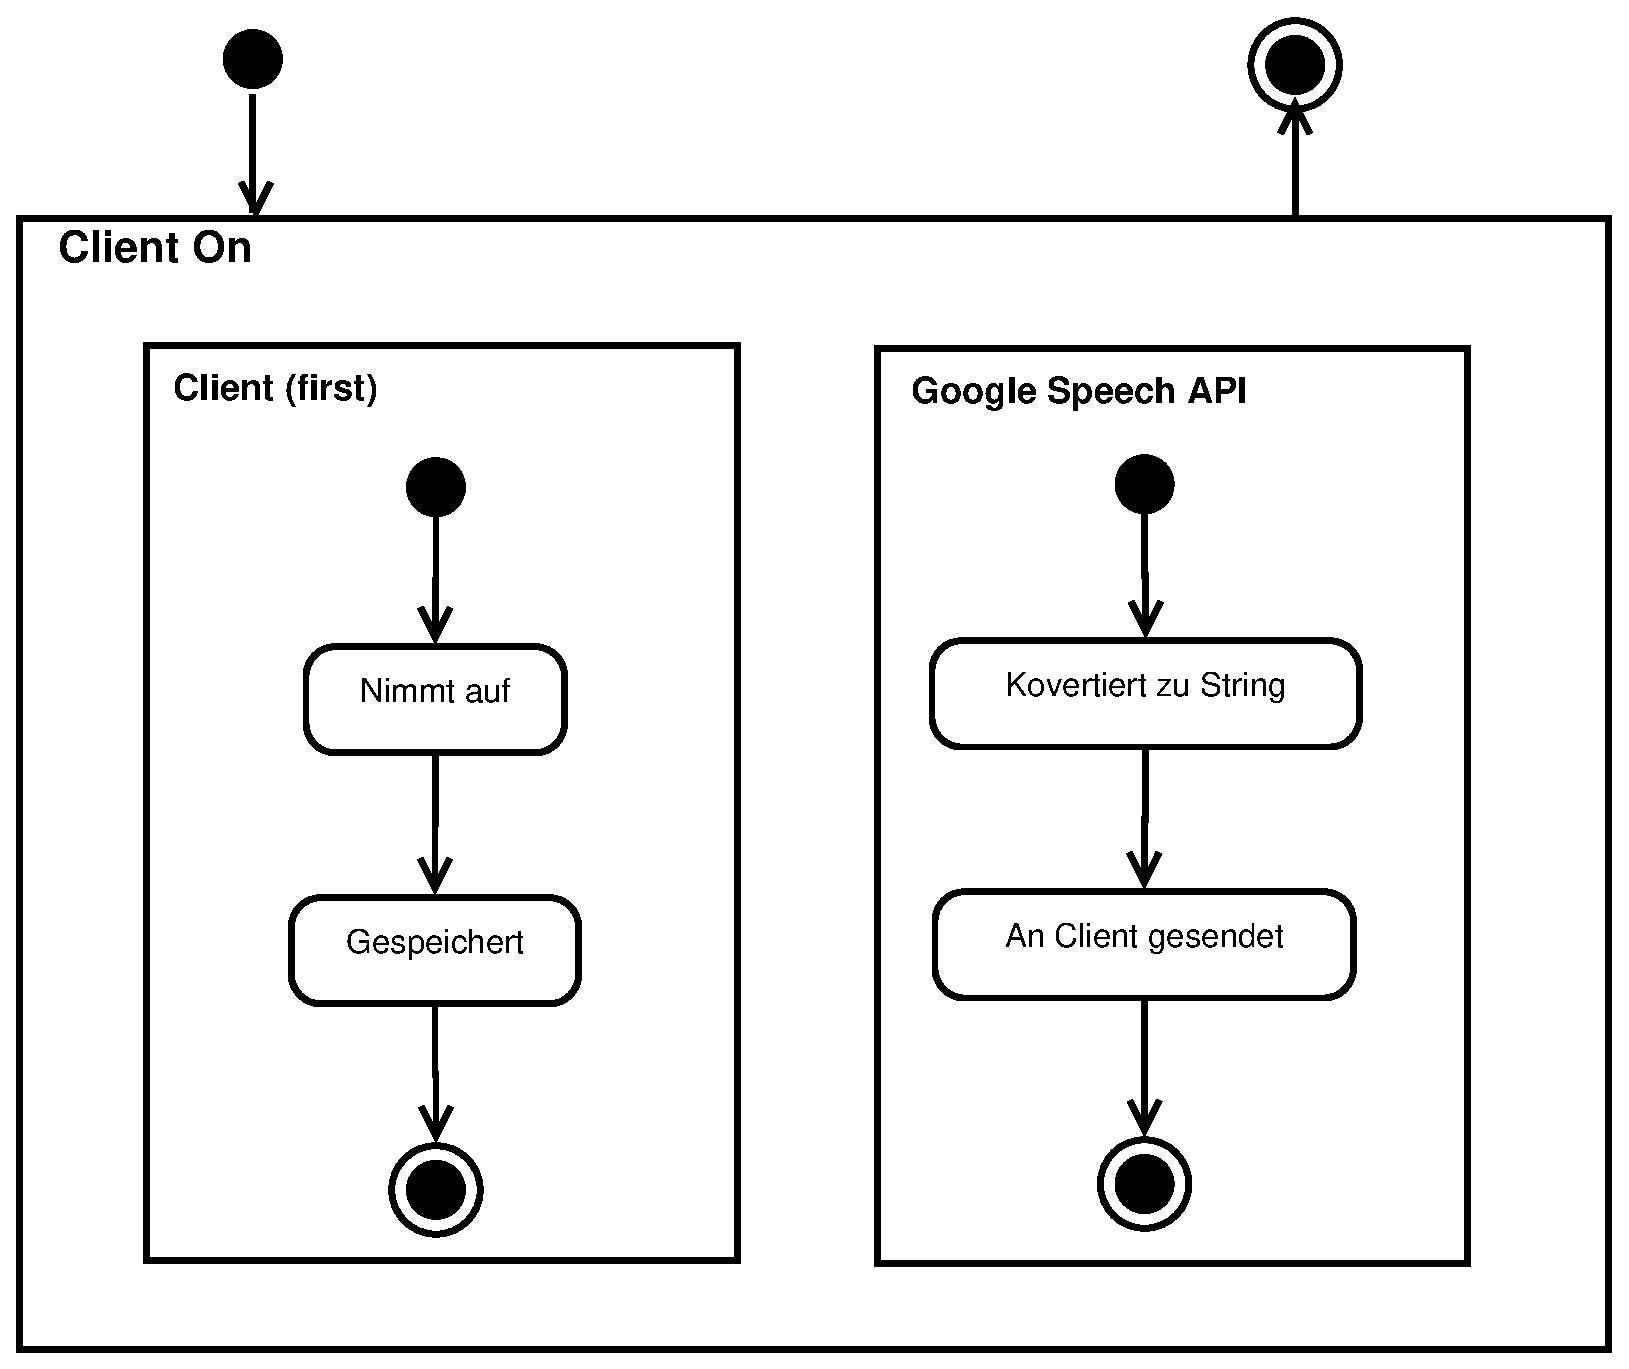
\includegraphics[width=.7\textwidth]{figures/client_chart.eps}
\caption{\textit{State Chart: Client}}
\label{fig:client_chart}
\end{figure}

\begin{figure}
\centering
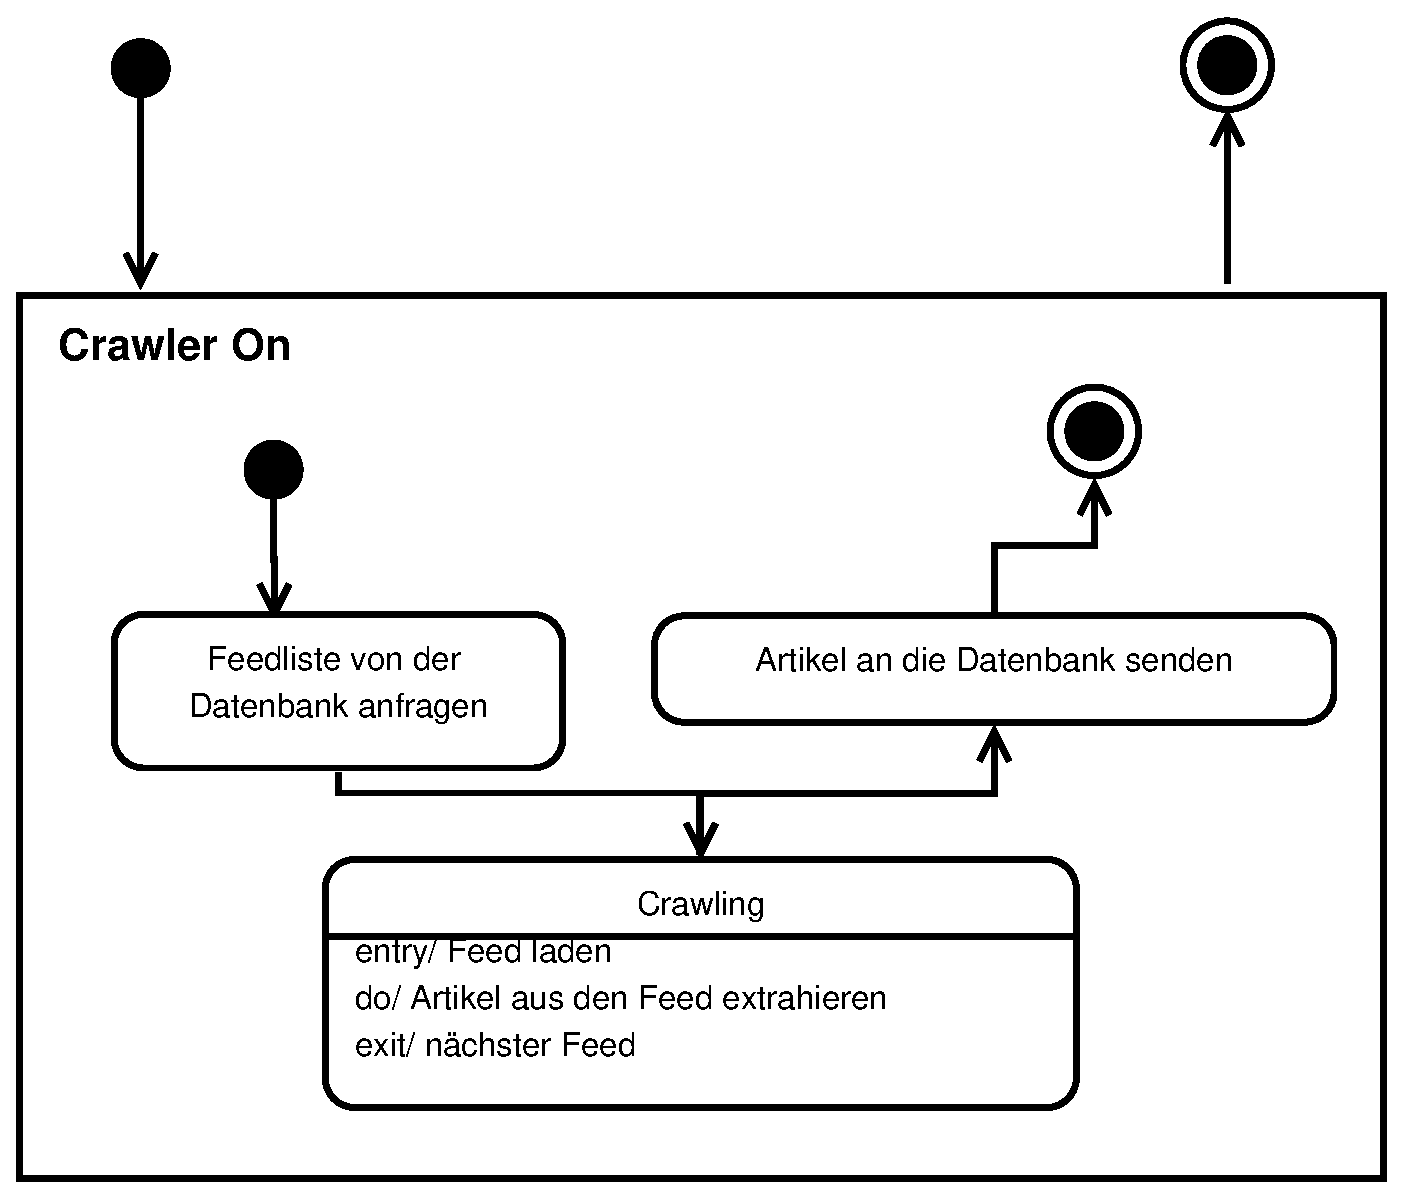
\includegraphics[width=0.7\textwidth]{figures/crawler_chart.eps}
\caption{\textit{State Chart: Crawler}}
\label{fig:crawler_chart}
\end{figure}



%!TEX root = ../TechnischerEntwurf.tex

\chapter{Verteilungsentwurf}

Das Front-End der Software sowie das mit gelieferte Admin-Tool wird über einen Webbrowser auf dem PC des Benutzers angezeigt. Die Daten dafür sind auf einem Server gespeichert. Um eingegebene Nutzerdaten zu überprüfen wird desweiteren eine Verbindung zum LDAP der TU Braunschweig aufgebaut.

\begin{figure}[ht]
\centering
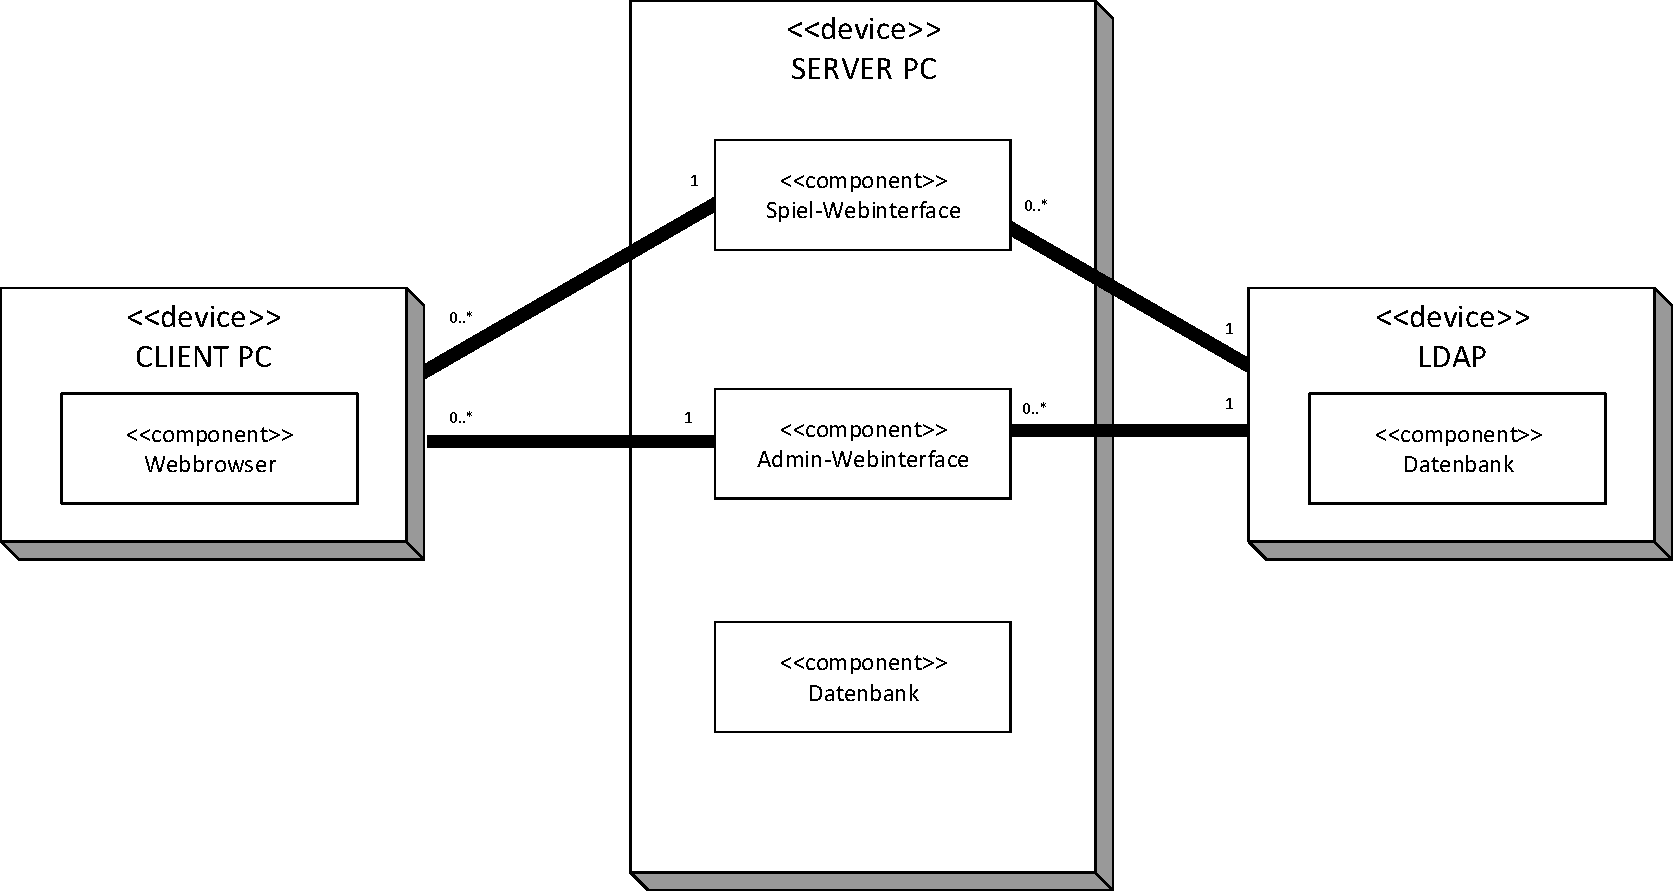
\includegraphics[width=1\textwidth]{figures/Verteilung1.pdf}
\caption{Verteilungsdiagramm für SQL-Alchemst}
\label{deployment}
\end{figure}

%!TEX root = ../Systementwurf2.tex

\chapter{Implementierungsentwurf}

Die Implementierung des \NewsGenie erfolgt eventbasiert. Der Austausch von
Nachrichtenobjekten dient dabei der Kommunikation unter den einzelnen
Komponenten. Im Folgenden werden die Komponenten und ihre Funktionen erläutert.

\begin{figure}[ht]
\centering
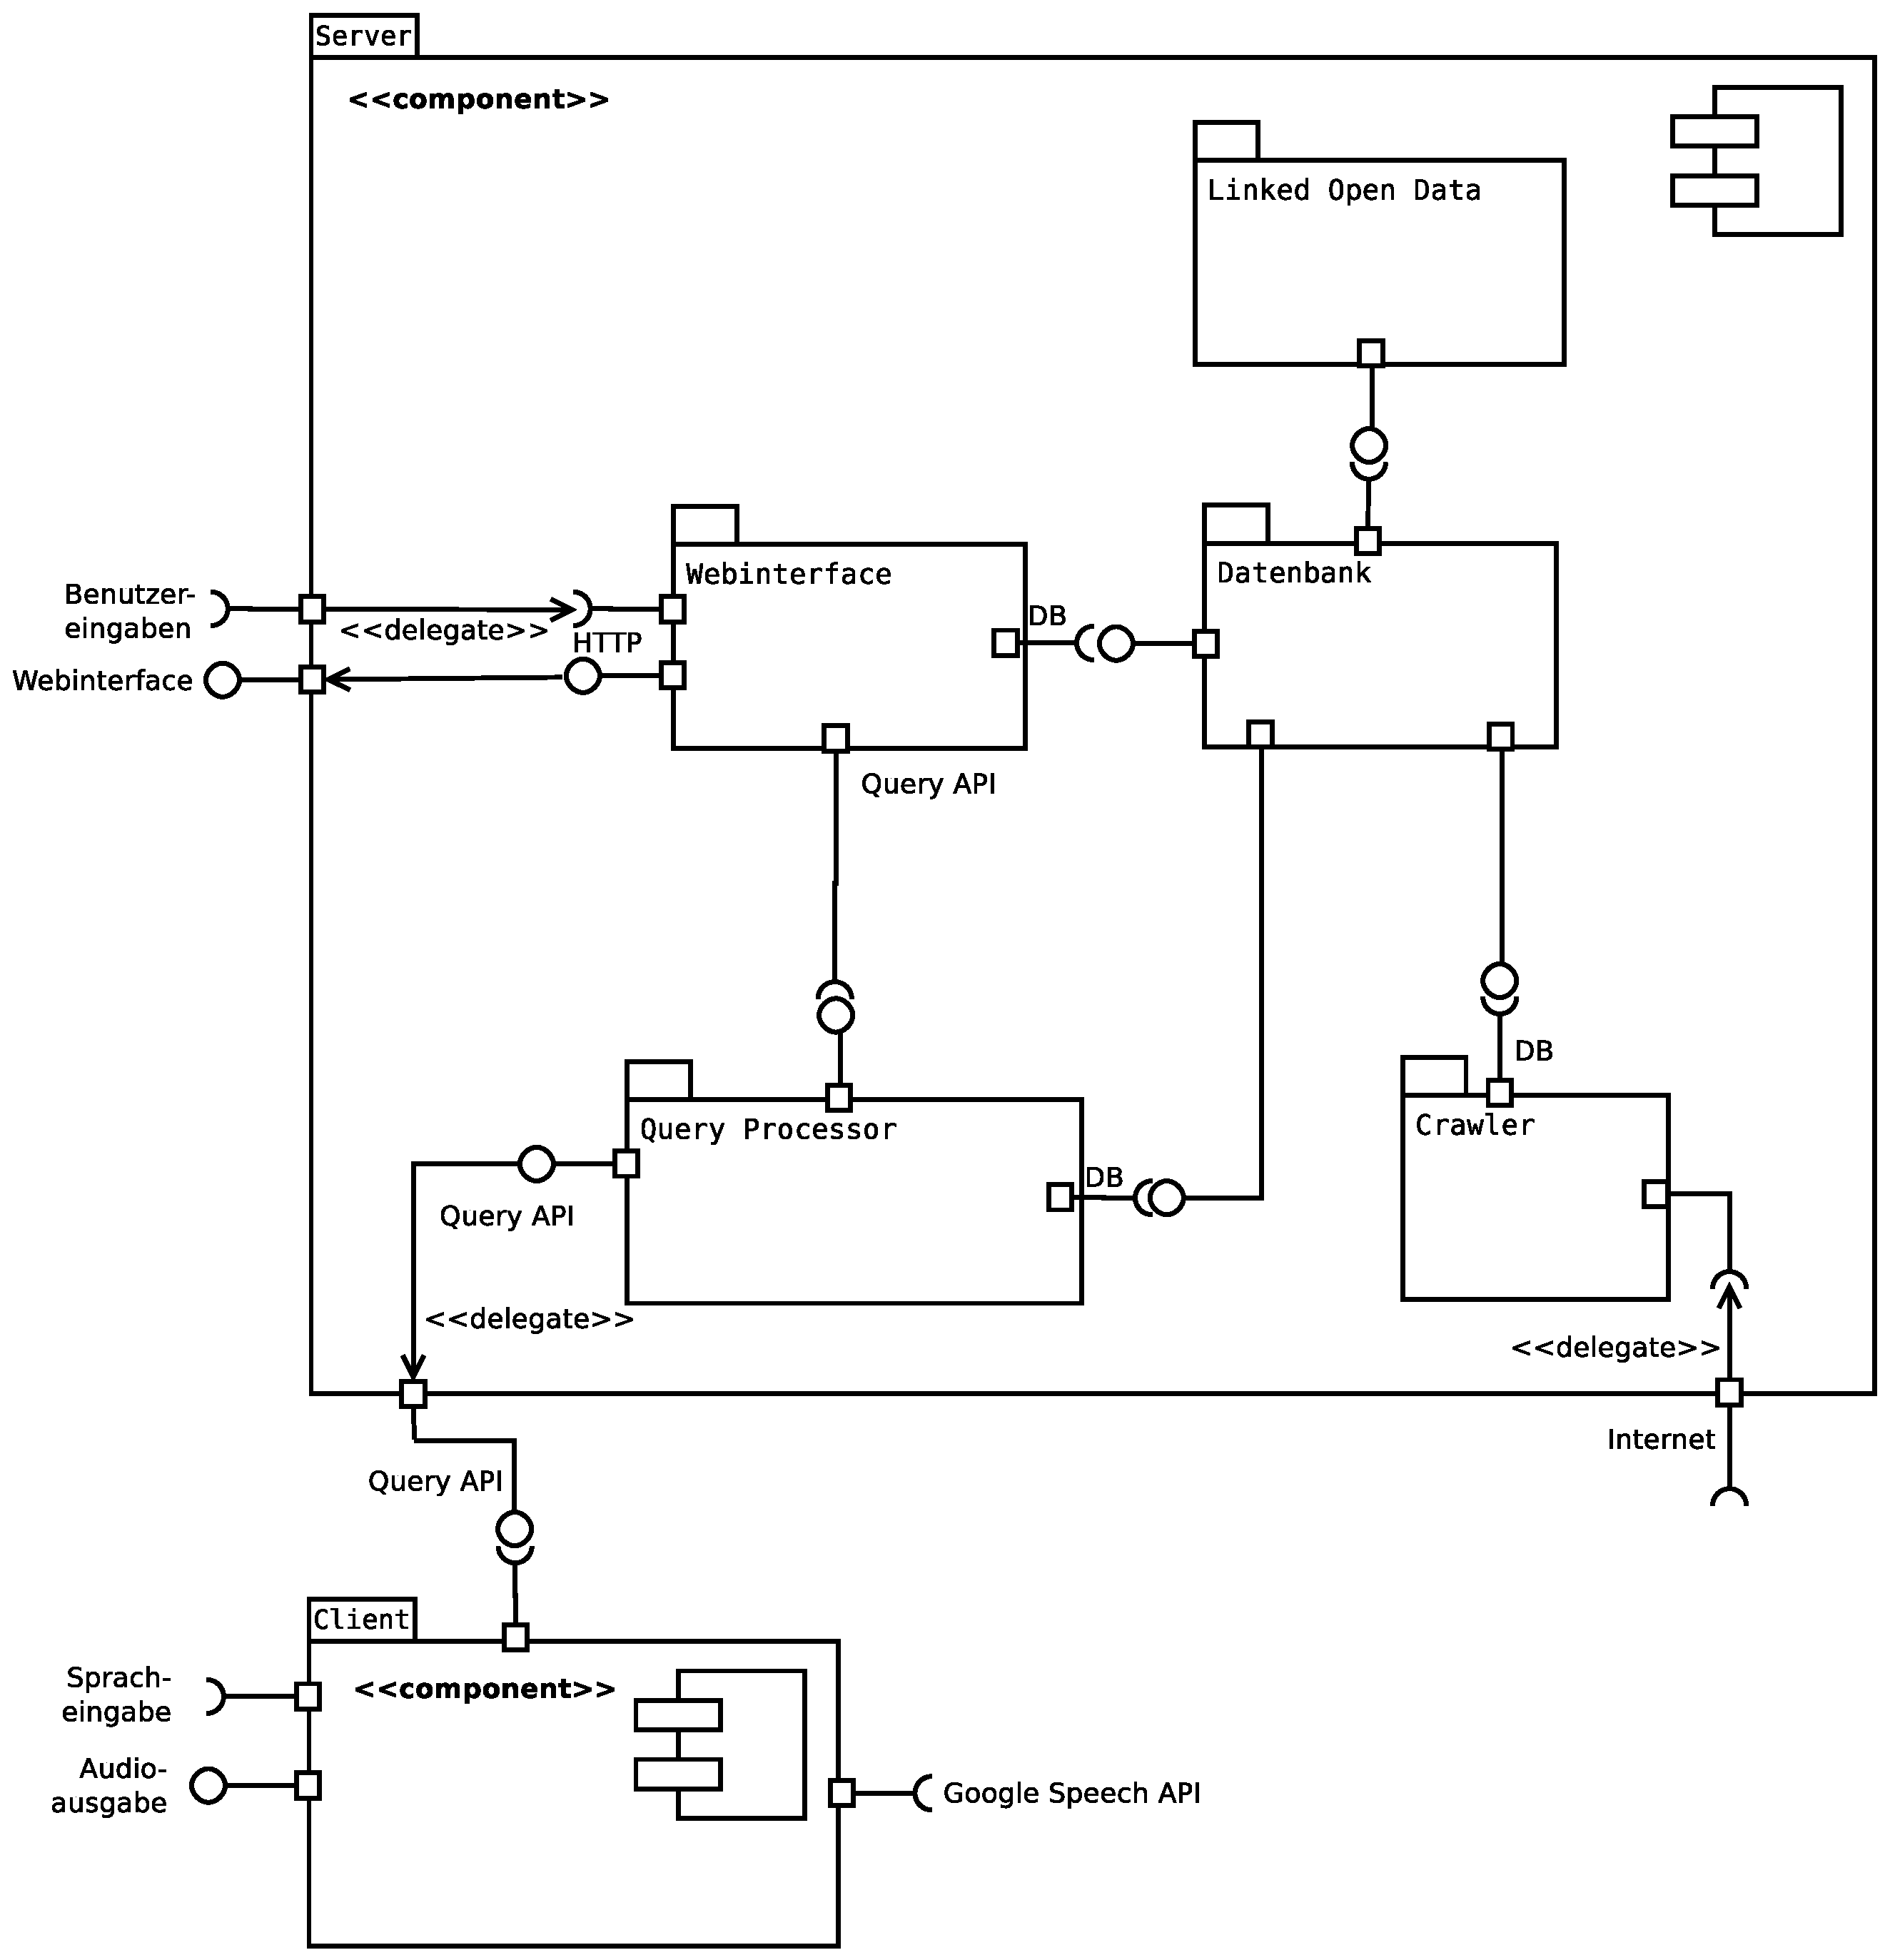
\includegraphics[width=1\textwidth]{Systementwurf/05_implementierungsentwurf/komponenten}
\caption{Komponentendiagramm, \textit{Komponentenaufteilung von \NewsGenie}}
\end{figure}

\begin{figure}[ht]
\centering
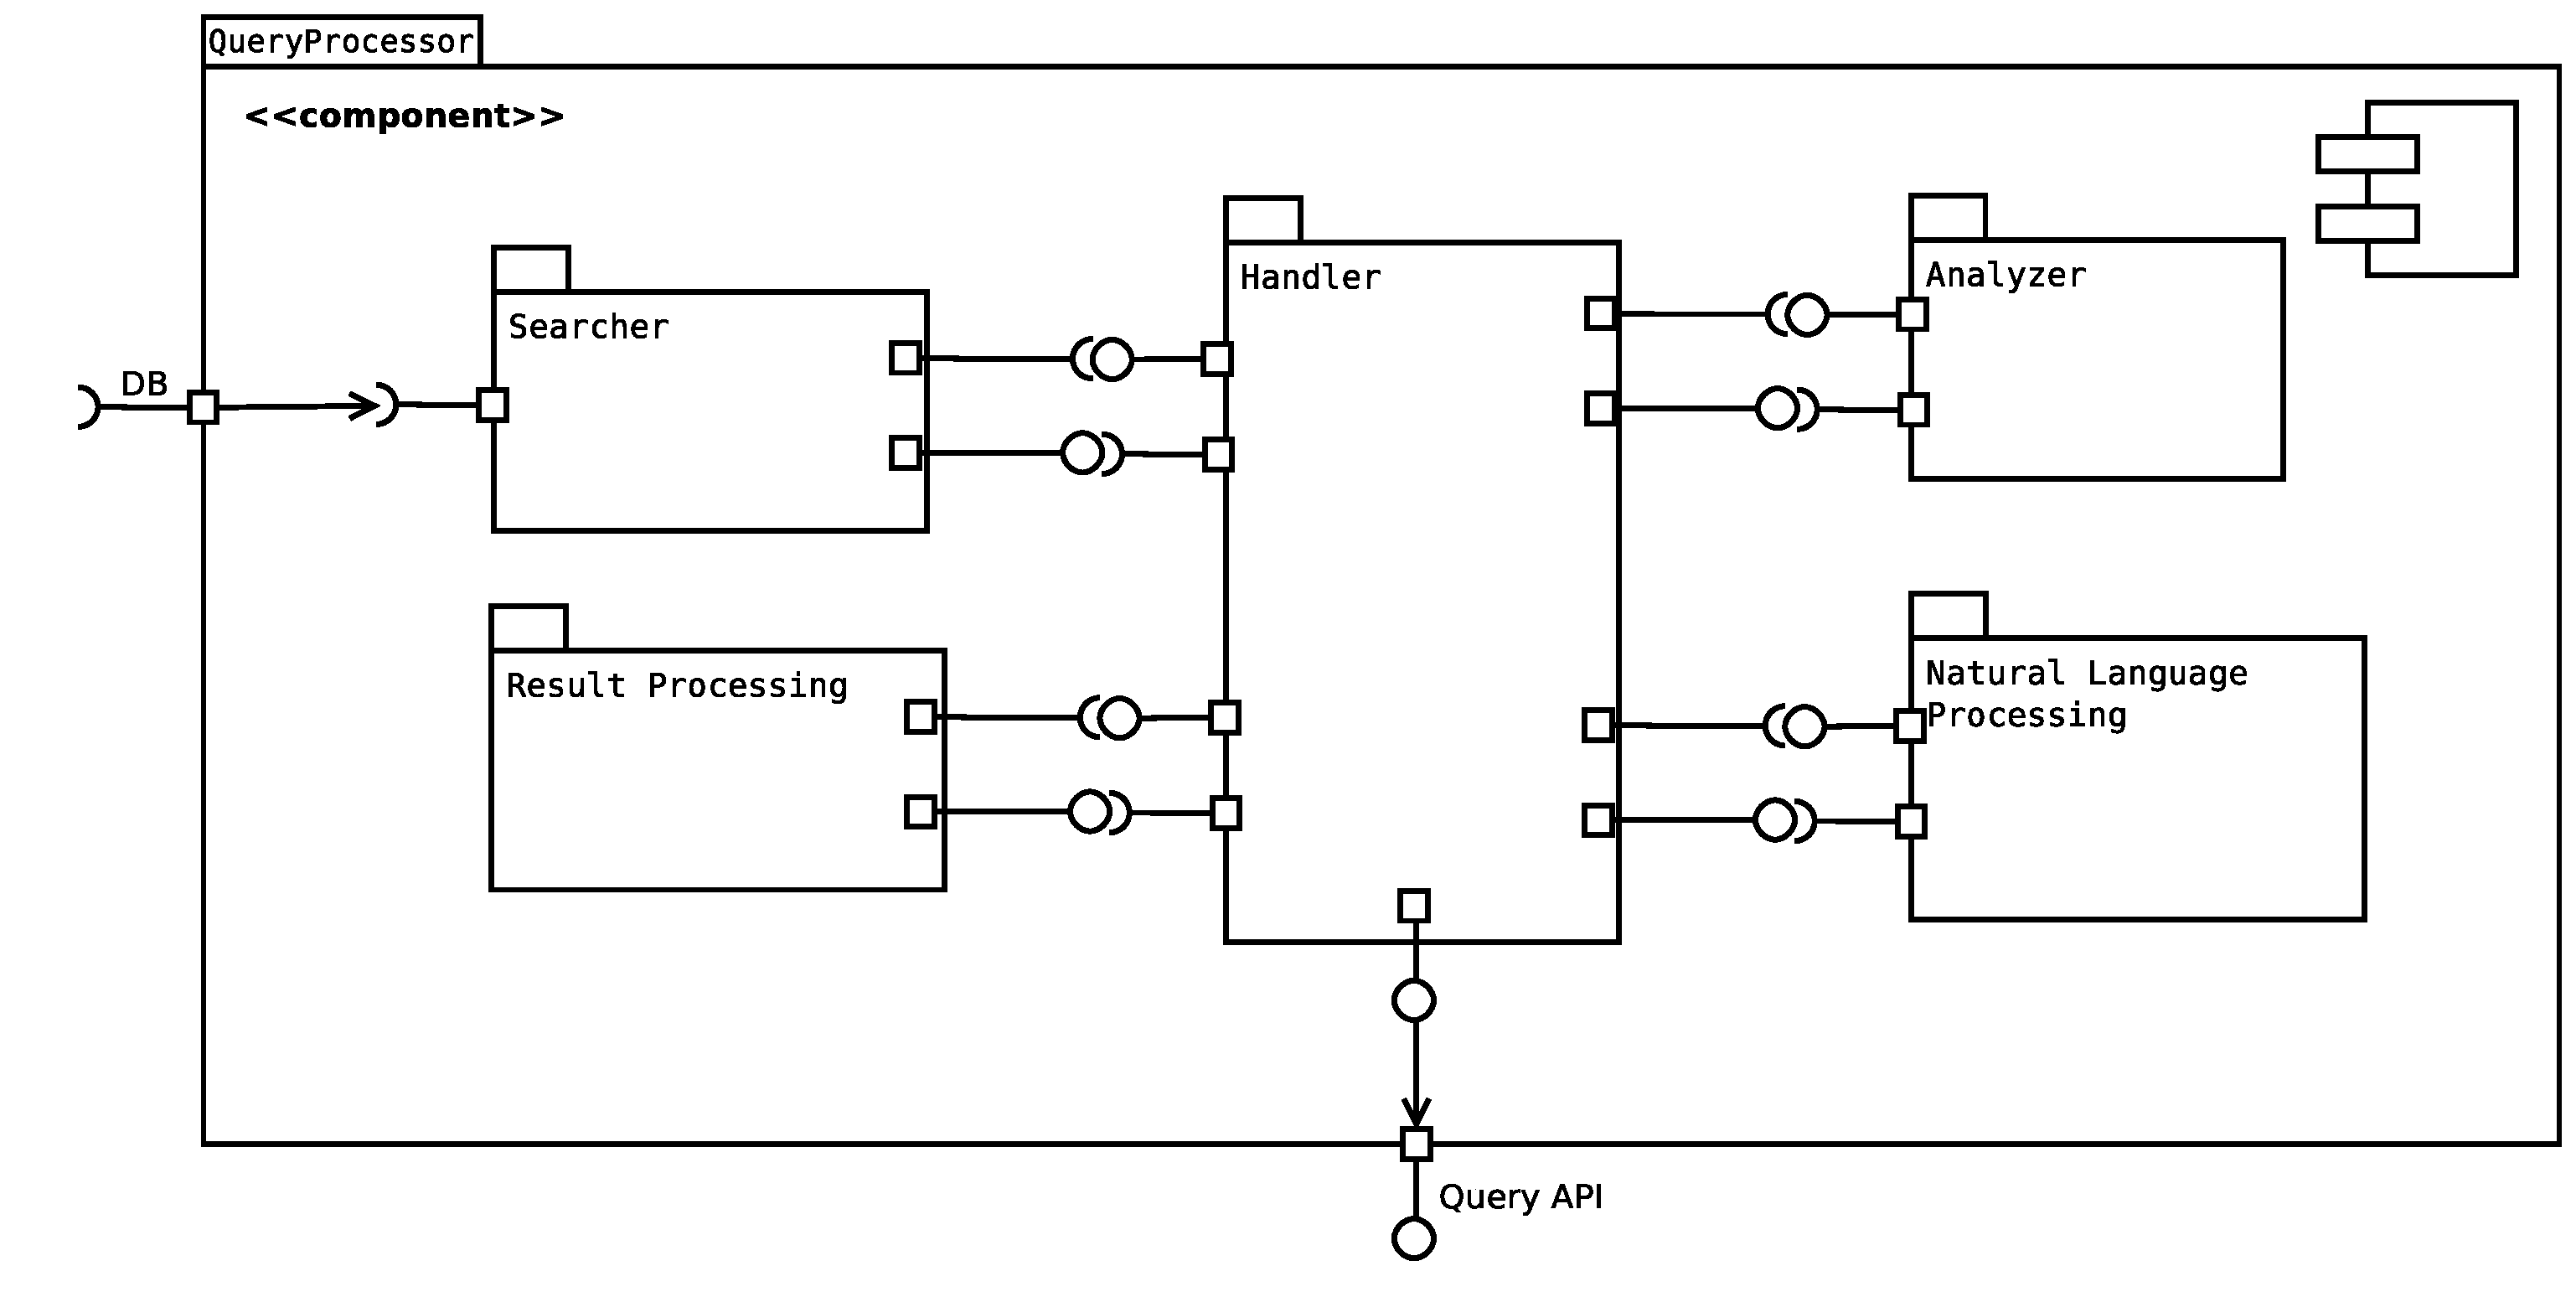
\includegraphics[width=1\textwidth]{Systementwurf/05_implementierungsentwurf/paket-queryprocessor}
\caption{Komponentendiagramm, \textit{Komponenten des Queryprocessors}}
\end{figure}

\FloatBarrier

% C10 Client

\section{Implementierung von Komponente $\langle$C10$\rangle$: Client}

Der Client dient als Frontend des \NewsGenie. Für die Kommunikation mit dem
Server wird das Akka-Framework genutzt. Der Client wird eventbasiert realisiert
und nach dem Start durch den \textit{ServerHandler} gesteuert.

\subsection{Paket-/Klassendiagramm}

\begin{figure}[ht]
\centering
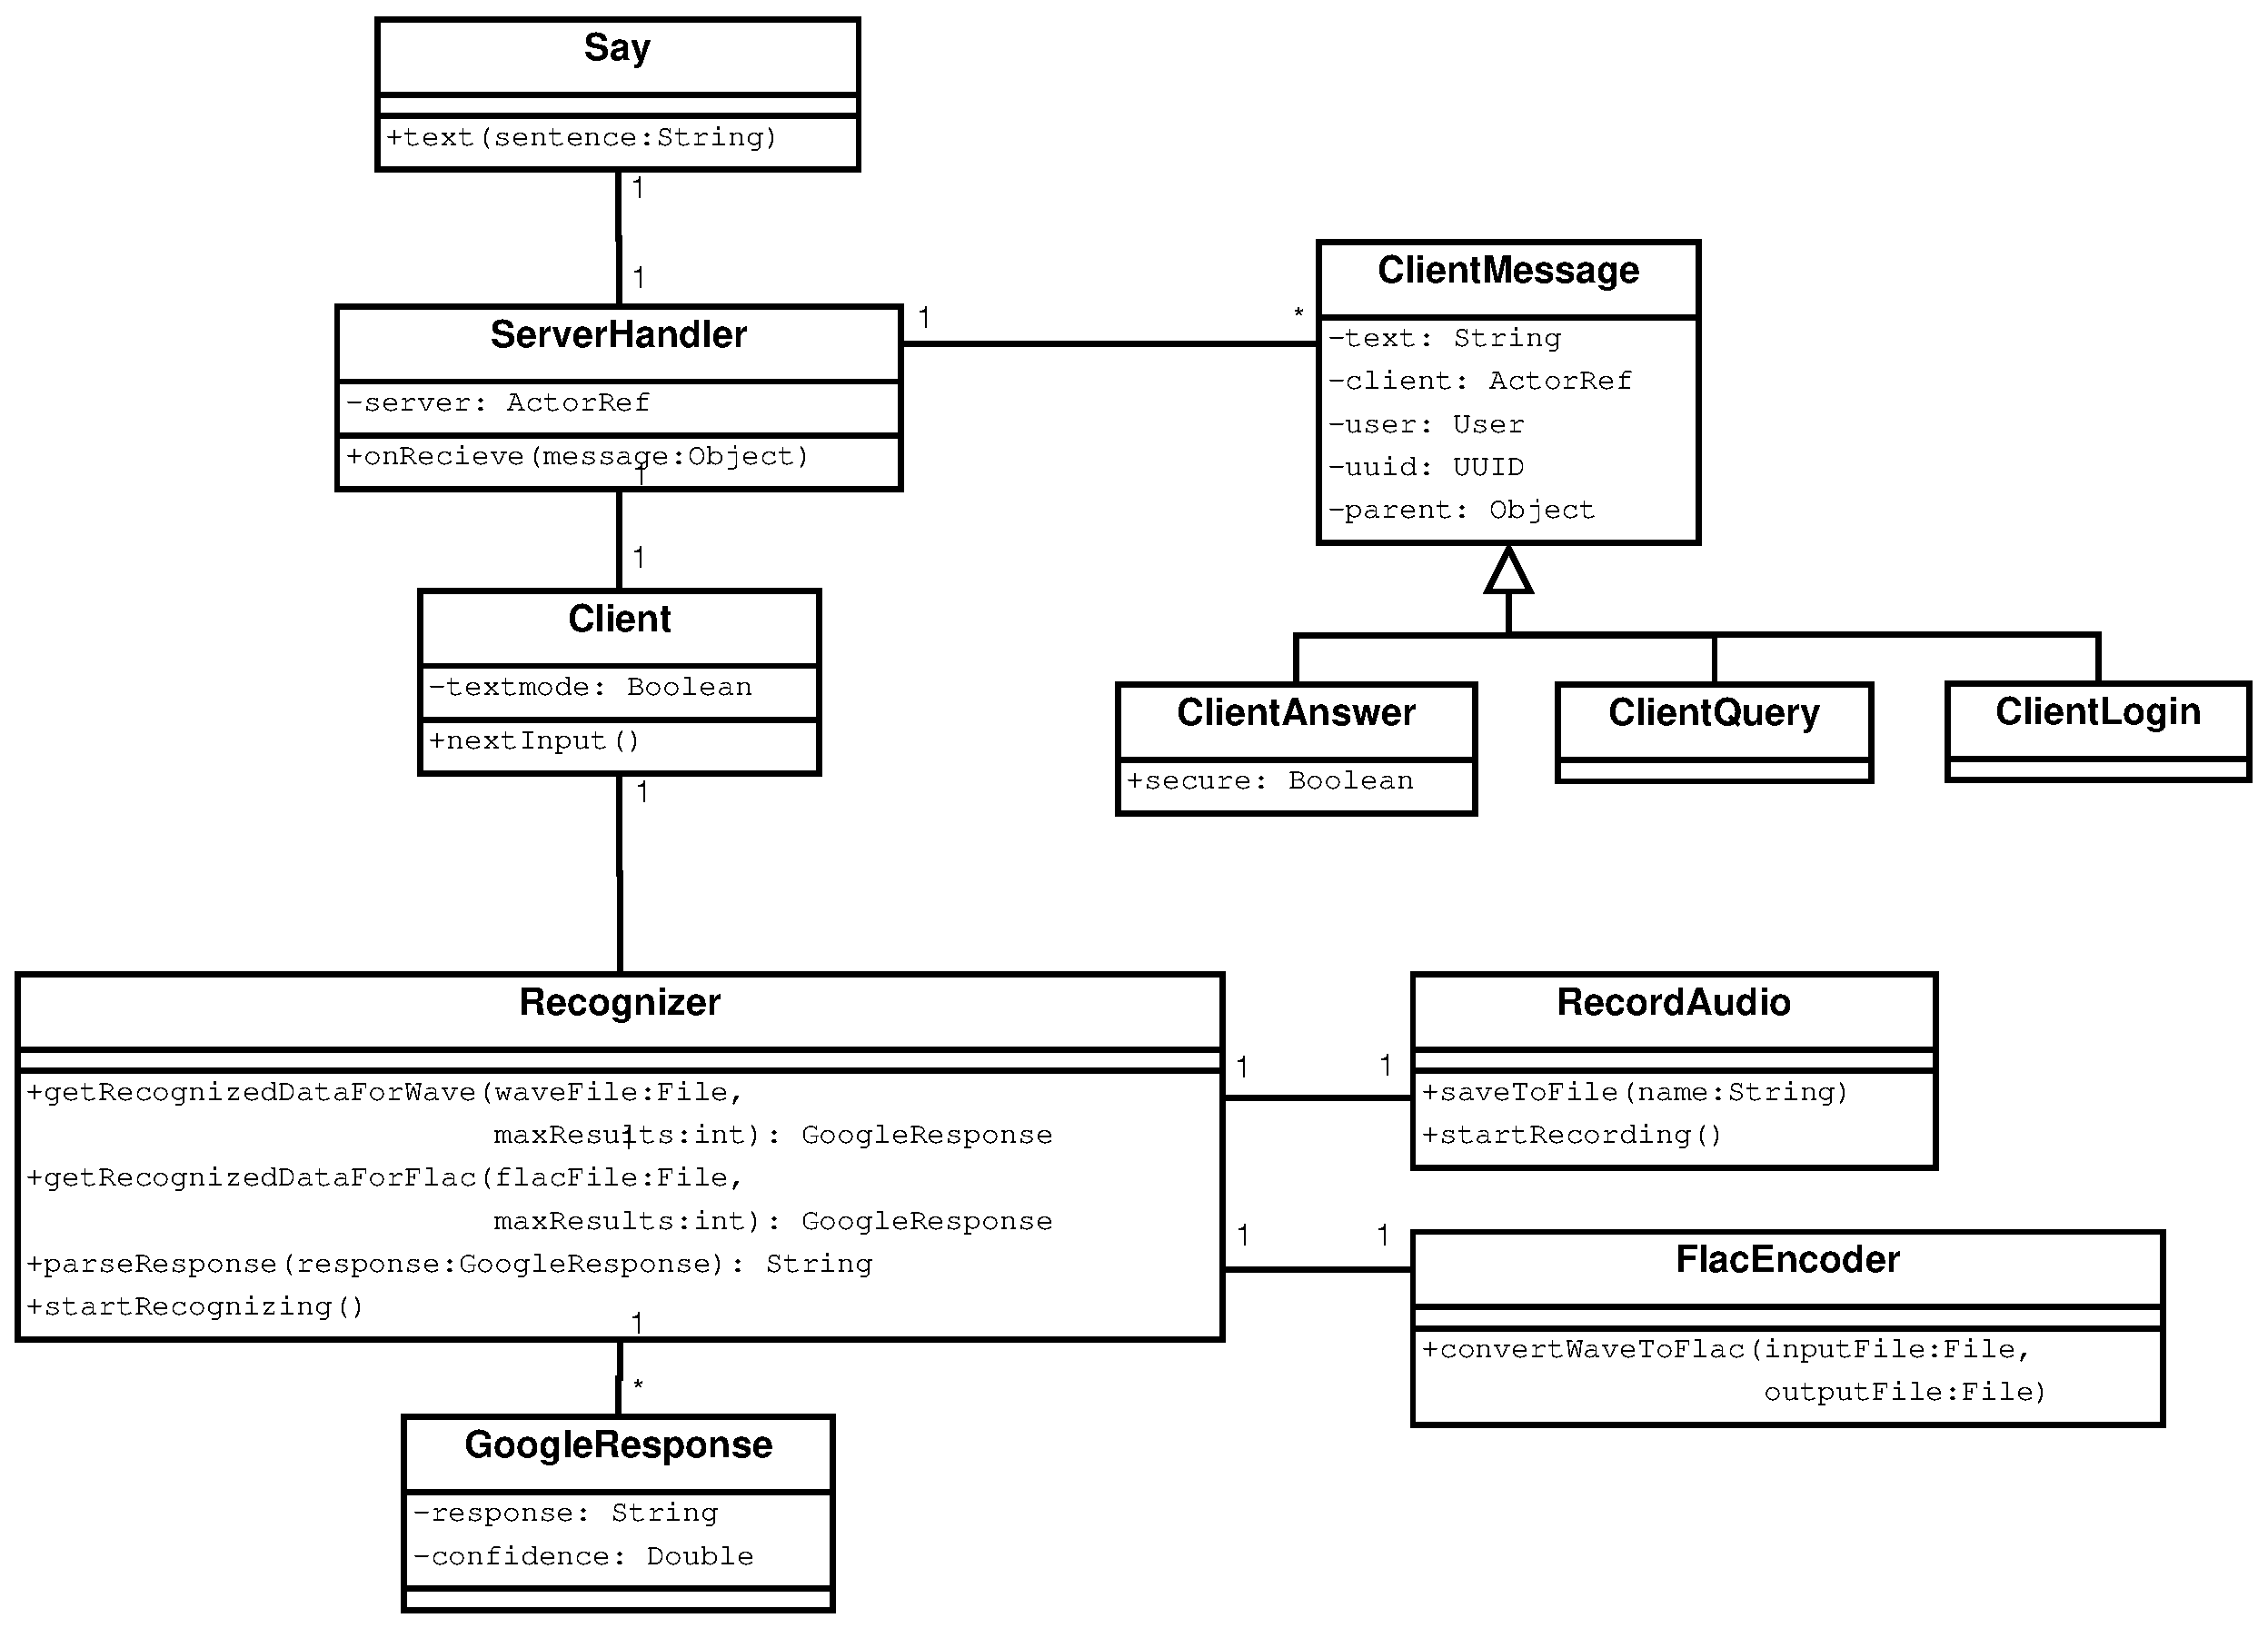
\includegraphics[width=1.03\textwidth]{Systementwurf/05_implementierungsentwurf/client-objekte}
\caption{Klassendiagramm für Komponente \ref{C10}}
\end{figure}

\subsection{Erläuterung}

Im Folgenden werden Attribute, Aufgaben und Kommunikationspartner für jede
Klasse des Clients kurz zu erläutern. Get-/Set-Methoden werden dabei nicht
berücksichtigt, sondern nur deren Attribute als \texttt{private} mit einem
Minuszeichen gekennzeichnet.

\pagebreak[4]
\begin{class}{10}{Client}
\item[Aufgabe]~\
Hauptklasse des Clients. Initialisierung der einzelnen Singleton-Objekte die zum
Bearbeiten einer Anfrage notwendig sind.
\item[Attribute]~\
\begin{itemize}
  \item \texttt{textmode}: falls \texttt{true} akzeptiert der Client
  Tastatureingaben statt Spracheingaben
\end{itemize}
\item[Operationen]~\
\begin{itemize}
  \item \texttt{nextInput()}: startet die nächste Eingabe durch Aufruf des
  \textit{Recognizers}. Der Aufruf erfolgt entweder per Tastendruck oder durch
  den \textit{ServerHandler}.
\end{itemize}
\item[Kommunikationspartner]~\
  \textit{Recognizer}, \textit{ServerHandler}
\end{class}

\begin{class}{10}{Recognizer}
\item[Aufgabe]~\
Realisiert die Umwandlung der Sprachbefehle in Text.
\item[Attribute]~\
keine
\item[Operationen]~\
\begin{itemize}
    \item \texttt{getRecognizedDataForWave(File waveFile, int maxResults)}
    schickt eine Wave-Datei an die Speech-API und erhält ein
    \texttt{GoogleResponse}-Objekt zurück.
    \item \texttt{getRecognizedDataForFlac(File flacFile, int maxResults)}
    schickt eine Flac-Datei an die Speech-API und erhält ein 
    \texttt{GoogleResponse}-Objekt zurück.
    \item \texttt{parseResponse(GoogleResponse response)} wertet ein
    \texttt{GoogleResponse}-Objekt aus und gibt die erkannte Anfrage als String
    zurück.
    \item \texttt{startRecognizing()} steuert den Ablauf einer Anfrage über
    Aufzeichnung und Erkennung und gibt einen String zurück.
\end{itemize}
\item[Kommunikationspartner]~\
\textit{RecordAudio}, \textit{FlacEncoder}, \textit{GoogleResponse}
\end{class}

\begin{class}{10}{RecordAudio}
\item[Aufgabe]~\
Steuert die Audioaufnahme und Speicherung. Diese Klasse ist als Singleton
ausgelegt.
\item[Attribute]~\
keine
\item[Operationen]~\
\begin{itemize}
    \item \texttt{saveToFile(String name)} speichert eine erfolgte Audioaufnahme
    als Wave-Datei.
    \item \texttt{startRecording()} startet die Aufnahme über das Mikrofon,
    bricht ab, wenn der Pegel unter ein Limit fällt.
\end{itemize}
\item[Kommunikationspartner]~\
\textit{Recognizer}
\end{class}

\begin{class}{10}{FlacEncoder}
\item[Aufgabe]~\
Singleton-Klasse zur Umwandlung von Wave in Flac-Dateien.
\item[Attribute]~\
keine
\item[Operationen]~\
\begin{itemize}
    \item \texttt{convertWaveToFlac(File inputFile, File outputFile)} wandelt
    eine Wave-Datei in eine Flac-Datei um.
\end{itemize}
\item[Kommunikationspartner]~\
\textit{Recognizer}
\end{class}

\begin{class}{10}{GoogleResponse}
\item[Aufgabe]~\
Speicherung der Google Speech-API Antwortdaten
\item[Attribute]~\
\begin{itemize}
    \item \texttt{response} Antwort der Speech-API als String
    \item \texttt{confidence} prozentuale Sicherheit der erfolgten Erkennung als
    Double-Wert
\end{itemize}
\item[Operationen]~\
keine
\item[Kommunikationspartner]~\
\textit{Recognizer}
\end{class}

\begin{class}{10}{ServerHandler}
\item[Aufgabe]~\
Singleton-Klasse für die Serverkommunikation. Der Nachrichtenaustausch erfolgt
durch das Senden von Objekten zwischen Server und Client.
\item[Attribute]~\
\begin{itemize}
    \item \texttt{server} Akka-ActorRef-Object, dass auf den Server verweist.
\end{itemize}
\item[Operationen]~\
\begin{itemize}
    \item \texttt{onRecieve(Object message)}
\end{itemize}
\item[Kommunikationspartner]~\
\textit{Client}, \textit{Say}, \textit{ClientMessage}
\end{class}

\begin{class}{10}{Say}
\item[Aufgabe]~\
Singleton-Klasse zur Ausgabe von Text als Sprache.
\item[Attribute]~\
keine
\item[Operationen]~\
\begin{itemize}
    \item \texttt{text(String sentence)} wandelt einen String in eine Wave-Datei
    um und spielt diese ab.
\end{itemize}
\item[Kommunikationspartner]~\

\end{class}

\begin{class}{10}{ClientMessage}
\item[Aufgabe]~\
Superklasse der Nachrichten, die zwischen Server und Client ausgetauscht werden.
\item[Attribute]~\
\begin{itemize}
    \item \texttt{text} Text der Nachricht als String.
    \item \texttt{client} Akka-ActorRef-Objekt mit Verweis auf den absendenden
    Client.
    \item \texttt{user} auf dem Client angemeldeter Benutzer als User-Objekt.
    \item \texttt{uuid} einzigartige ID zur Identifikation der Nachricht.
    \item \texttt{parent} enthält evtl. ein Objekt, dass der Server zur weiteren
    Auswertung mit an den Client übergeben möchte, z.B. eine Liste von Artikeln.
\end{itemize}
\item[Operationen]~\
keine
\item[Kommunikationspartner]~\
\textit{ServerHandler}
\end{class}

\begin{class}{10}{ClientAnswer}
\item[Aufgabe]~\
Objekt zur Übertragung einer Serverantwort an den Client
\item[Attribute]~\
Attribute der Superklasse, sowie
\begin{itemize}
    \item \texttt{secure} Bool'scher Wert, \textit{true} falls die Antwort
    sicher ist und ohne Rückfrage auskommt.
\end{itemize}
\item[Operationen]~\
keine
\item[Kommunikationspartner]~\
\textit{ServerHandler}
\end{class}

\begin{class}{10}{ClientQuery}
\item[Aufgabe]~\
Objekt zur Übertragung einer Clientanfrage an den Server
\item[Attribute]~\
nur Attribute der Superklasse
\item[Operationen]~\
keine
\item[Kommunikationspartner]~\
\textit{ServerHandler}
\end{class}

\begin{class}{10}{ClientLogin}
\item[Aufgabe]~\
Objekt zur Übertragung einer Loginanfrage vom Client zum Server
\item[Attribute]~\
nur Attribute der Superklasse
\item[Operationen]~\
keine
\item[Kommunikationspartner]~\
\textit{ServerHandler}
\end{class}

\FloatBarrier

% C20 Webinterface
%!TEX root = ../../Systementwurf2.tex

\section{Implementierung von Komponente <C20>: Webinterface}

Das Webinterface stellt eine Schnittstelle für Benutzer und Administratoren bereit, in dem sie ihre Einstellungen verwalten können. Es wird mit dem Play-Framework implementiert und kommuniziert mit dem Server eventbasiert mittels Akka.

\subsection{Paket-/Klassendiagramm}

\begin{figure}[ht]
\centering
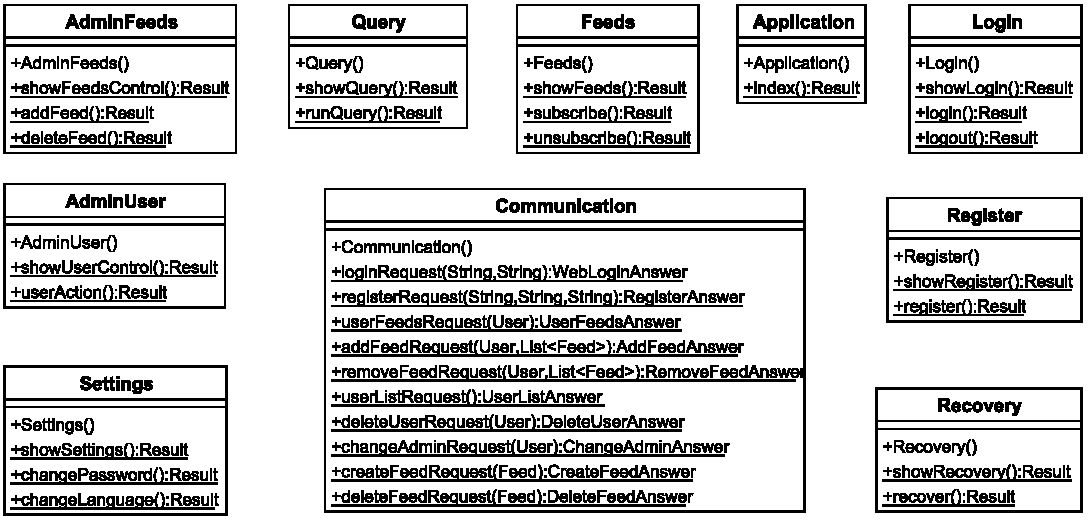
\includegraphics[width=1.03\textwidth]{Systementwurf/05_implementierungsentwurf/webinterface}
\caption{Klassendiagramm für Komponente \ref{C20}}
\end{figure}

\subsection{Erläuterung}

Im Folgenden werden Attribute, Aufgaben und Kommunikationspartner für jede Klasse des Webinterfaces kurz erläutert.\\
Die Funktionen der Klassen (außer Communication) besitzen keine Parameter, da diese per HTTP übertragen werden.

\begin{class}{10}{Communication}
\item[Aufgabe]~\
Die Communication-Klasse ist für die Kommunikation mit dem Server zuständig.
\item[Attribute]~\ keine
\item[Operationen]~\
\begin{itemize}
  \item \texttt{loginRequest(String, String)}: Sendet eine Anfrage, um einen Benutzer einzuloggen.
  \item \texttt{registerRequest(String, String, String)}: Sendet eine Anfrage, um einen neuen Benutzer zu registrieren.
  \item \texttt{userFeedsRequest(User)}: Sendet eine Anfrage, um alle Feeds eines Benutzers zu erhalten.
  \item \texttt{addFeedRequest(User, List<Feed>)}: Sendet eine Anfrage, um einen Benutzer mit Feeds zu verknüpfen.
  \item \texttt{removeFeedRequest(User, List<Feed>)}: Sendet eine Anfrage, um die Verknüpfungen zwischen einem Benutzer und Feeds zu entfernen.
  \item \texttt{userListRequest()}: Sendet eine Anfrage, um eine Liste aller Benutzer zu erhalten.
  \item \texttt{deleteUserRequest(User)}: Sendet eine Anfrage, um einen Benutzer zu löschen.
  \item \texttt{changeAdminRequest(User)}: Sendet eine Anfrage, um einem Benutzer Administratorenrechte zu gewähren oder zu entziehen.
  \item \texttt{createFeedRequest(Feed)}: Sendet eine Anfrage, um einen neuen Feed anzulegen.
  \item \texttt{deleteFeedRequest(Feed)}: Sendet eine Anfrage, um einen Feed zu löschen.
\end{itemize}
\item[Kommunikationspartner]~\
  \textit{ServerHandler}
\end{class}

\begin{class}{20}{AdminFeeds}
\item[Aufgabe]~\
Die AdminFeeds-Klasse stellt die Webseite zum Administrieren von Feeds zur Verfügung.
\item[Attribute]~\ keine
\item[Operationen]~\
\begin{itemize}
    \item \texttt{showFeedsControl()} Zeigt die Webseite an.
    \item \texttt{addFeed()} Sendet eine Anfrage, einen neuen Feed zu erstellen.
    \item \texttt{deleteFeed()} Sendet eine Anfrage, einen Feed zu löschen.
\end{itemize}
\item[Kommunikationspartner]~\ keine
\end{class}

\begin{class}{30}{AdminUser}
\item[Aufgabe]~\
Die AdminUser-Klasse stellt die Webseite zum Administrieren von Benutzern zur Verfügung.
\item[Attribute]~\ keine
\item[Operationen]~\
\begin{itemize}
    \item \texttt{showUserControl()} Zeigt die Webseite an.
    \item \texttt{userAction()} Löscht einen Benutzer oder ändert seinen Admin-Status.
\end{itemize}
\item[Kommunikationspartner]~\ keine
\end{class}

\begin{class}{40}{Settings}
\item[Aufgabe]~\
Die Settings-Klasse stellt die Webseite zum Ändern der Benutzereinstellungen zur Verfügung.
\item[Attribute]~\ keine
\item[Operationen]~\
\begin{itemize}
    \item \texttt{showSettings()} Zeigt die Webseite an.
    \item \texttt{changePassword()} Sendet eine Anfrage, das Passwort zu ändern.
    \item \texttt{changeLanguage()} Sendet eine Anfrage, die Sprache zu ändern.
\end{itemize}
\item[Kommunikationspartner]~\ keine
\end{class}

\begin{class}{50}{Query}
\item[Aufgabe]~\
Die Query-Klasse stellt die Webseite zum Stellen eines Text-Queries zur Verfügung.
\item[Attribute]~\ keine
\item[Operationen]~\
\begin{itemize}
    \item \texttt{showQueryl()} Zeigt die Webseite an.
    \item \texttt{runQuery()} Sendet eine Anfrage mit einem Text-Query.
\end{itemize}
\item[Kommunikationspartner]~\ keine
\end{class}

\begin{class}{60}{Feeds}
\item[Aufgabe]~\
Die Feeds-Klasse stellt die Webseite zum Verwalten der Feedeinstellungen zur Verfügung.
\item[Attribute]~\ keine
\item[Operationen]~\
\begin{itemize}
    \item \texttt{showFeedsl()} Zeigt die Webseite an.
    \item \texttt{subscribe()} Sendet eine Anfrage, Feeds zu abonnieren.
    \item \texttt{dleteFeed()} Sendet eine Anfrage, Feeds zu deabonnieren.
\end{itemize}
\item[Kommunikationspartner]~\ keine
\end{class}

\begin{class}{70}{Application}
\item[Aufgabe]~\
Die Application-Klasse stellt die Startwebseite zur Verfügung.
\item[Attribute]~\ keine
\item[Operationen]~\
\begin{itemize}
    \item \texttt{index()} Zeigt die Startseite an.
\end{itemize}
\item[Kommunikationspartner]~\ keine
\end{class}

\begin{class}{80}{Login}
\item[Aufgabe]~\
Die Login-Klasse stellt die Webseite zum Einloggen zur Verfügung.
\item[Attribute]~\ keine
\item[Operationen]~\
\begin{itemize}
    \item \texttt{showLogin()} Zeigt die Webseite an.
    \item \texttt{login()} Sendet eine Anfrage, einen Benutzer einzuloggen.
    \item \texttt{logout()} Sendet eine Anfrage, einen Benutzer auszuloggen.
\end{itemize}
\item[Kommunikationspartner]~\ keine
\end{class}

\begin{class}{90}{Register}
\item[Aufgabe]~\
Die Register-Klasse stellt die Webseite zum Registrieren zur Verfügung.
\item[Attribute]~\ keine
\item[Operationen]~\
\begin{itemize}
    \item \texttt{showRegister()} Zeigt die Webseite an.
    \item \texttt{register()} Sendet eine Anfrage, einen neuen Benutzer zu registrieren.
\end{itemize}
\item[Kommunikationspartner]~\ keine
\end{class}

\begin{class}{100}{Recovery}
\item[Aufgabe]~\
Die Recovery-Klasse stellt die Webseite zum Wiederherstellen des Passworts zur Verfügung.
\item[Attribute]~\ keine
\item[Operationen]~\
\begin{itemize}
    \item \texttt{showRecovery()} Zeigt die Webseite an.
    \item \texttt{recover()} Sendet eine Anfrage, das Passwort wiederherzustellen.
\end{itemize}
\item[Kommunikationspartner]~\ keine
\end{class}

% C30 Datenbank
%!TEX root = ../../Systementwurf2.tex

\section{Implementierung von Komponente <C30>: Datenbank}

Die Datenbankkomponente dient zur Kommunikation mit dem Virtuoso Triplestore und dem Apache Lucene Index. Die Kommunikation mit den anderen Komponenten erfolgt eventbasiert mit Hilfe des Akka-Frameworks.

\subsection{Paket-/Klassendiagramm}

\begin{figure}[ht]
\centering
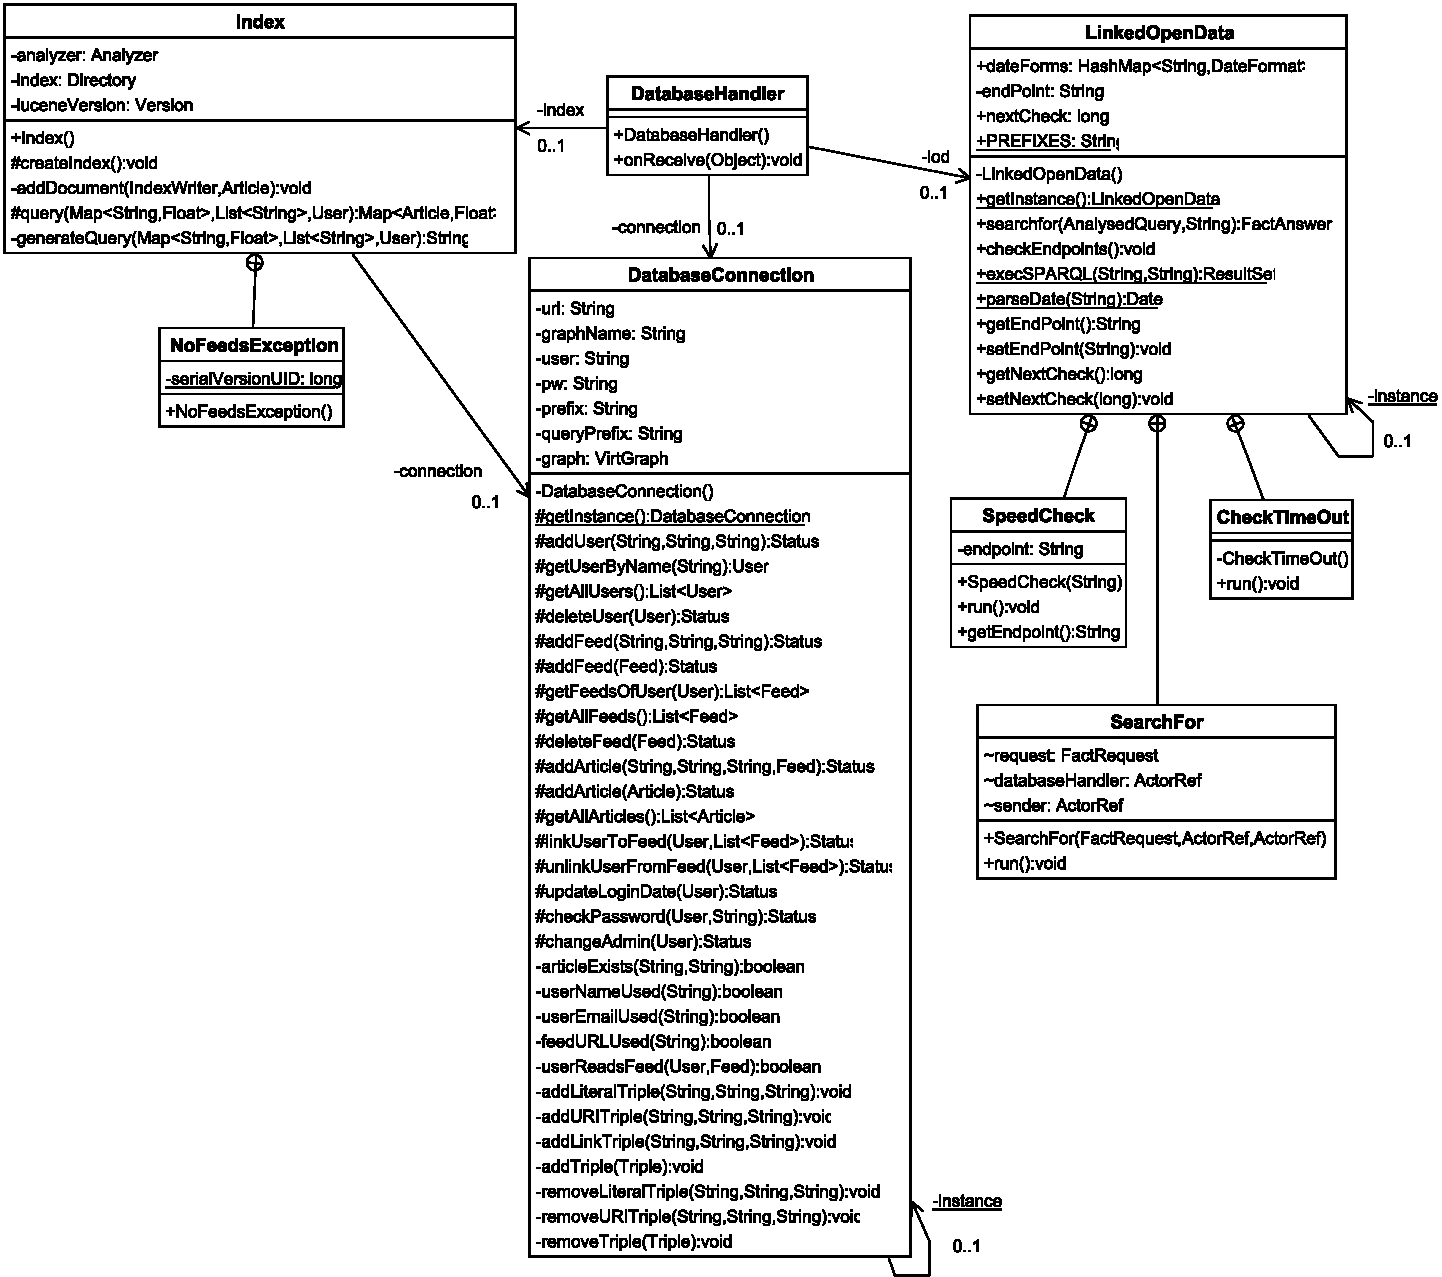
\includegraphics[width=1.03\textwidth]{Systementwurf/05_implementierungsentwurf/database}
\caption{Klassendiagramm für Komponente \ref{C30}}
\end{figure}

\subsection{Erläuterung}

Im Folgenden werden Attribute, Aufgaben und Kommunikationspartner für jede
Klasse der Datenbankkomponente kurz erläutert.

\begin{class}{10}{DatabaseHandler}
\item[Aufgabe]~\
Die DatabaseHandler-Klasse ist die Hauptklasse der Datenbankkomponente. Sie nimmt Anfragen der anderen Komponenten mittels der onReceive() Methode entgegen und sendet Antworten auf diese Anfragen.
\item[Attribute]~\
\begin{itemize}
  \item \texttt{connection}: Referenz auf den \textit{DatabaseConnection}-Singleton.
  \item \texttt{index}: Referenz auf ein \textit{Index}-Objekt.
  \item \texttt{lod}: Referenz auf den \textit{LinkedOpenData}-Singleton.
\end{itemize}
\item[Operationen]~\
\begin{itemize}
  \item \texttt{onReceive()}: nimmt Anfragen anderer Komponenten entgegen und beantwortet sie.
\end{itemize}
\item[Kommunikationspartner]~\
  \textit{DatabaseConnection}, \textit{Index}, \textit{LinkedOpenData}, \textit{Searcher}, \textit{CrawlerHandler}, \textit{ManagementHandler}
\end{class}

\begin{class}{20}{DatabaseConnection}
\item[Aufgabe]~\
Die DatabaseConnection-Klasse enthält die verschiedenen SPARQL-Queries an den Virtuoso-Triplestore.
\item[Attribute]~\
\begin{itemize}
  \item \texttt{instance}: Referenz auf den \textit{DatabaseConnection}-Singleton.
  \item \texttt{url}: URL unter der die Virtuoso-Datenbank erreicht werden kann.
  \item \texttt{graphName}: Name des RDF-Graphen auf dem gearbeitet wird.
  \item \texttt{user}: Virtuoso-Benutzername.
  \item \texttt{pw}: Virtuoso-Benutzerpasswort.
  \item \texttt{prefix}: Prefix für URI Graphenknoten.
  \item \texttt{queryPrefix}: Prefix für URI Graphenknoten in Queries.
  \item \texttt{graph}: Referenz auf den RDF-Graphen auf dem gearbeitet wird.
\end{itemize}
\item[Operationen]~\
\begin{itemize}
    \item \texttt{getInstance()}  Liefert die Singleton-Instanz.
    \item \texttt{addUser(String, String, String)} Legt einen neuen Benutzer in der Datenbank an.
    \item \texttt{getUserByName(String)} Liefert den Benutzer mit dem angegebenen Namen.
    \item \texttt{getAllUsers()} Liefert alle exisistierenden Benutzer.
    \item \texttt{deleteUser(User)} Löscht den angegebenen Benutzer.
    \item \texttt{addFeed(String, String, String)} Legt einen neuen Feed in der Datenbank an.
    \item \texttt{addFeed(Feed)} Legt einen neuen Feed in der Datenbank an.
    \item \texttt{getFeedsOfUser(User)} Liefert die Feeds, die der angegebene Benutzer abonniert hat.
    \item \texttt{getAllFeeds()} Liefert alle existierenden Feeds.
    \item \texttt{deleteFeed(Feed)} Löscht den angegebenen Feed.
    \item \texttt{addArticle(String, String, String, Feed)} Legt einen neuen Artikel in der Datenbank an.
    \item \texttt{addArticle(Article)} Legt einen neuen Artikel in der Datenbank an.
    \item \texttt{getallArticles()} Liefert alle existierenden Artikel.
    \item \texttt{linkUserToFeed(User, List<Feed>)} Verknüpft den angegebenen Benutzer mit den Feeds aus der Liste.
    \item \texttt{unlinkUserFromFeed(User, List<Feed>)} Löscht die Verknüpfungen zwischen dem angegebenen Benutzer und den Feeds aus der Liste.
    \item \texttt{updateLoginDate(User)} Ändert das Datum des letzten Logins des angegebenen Benutzers auf die momentane Zeit.
    \item \texttt{checkPassword(User, String)} Prüft, ob der angegebene Benutzer das angegebene Passwort verwendet.
    \item \texttt{changeAdmin(User)} Ändert den Admin-Status des angegebenen Benutzers.
    \item Hilfsfunktionen: Die Klasse enthält einige private Hilfsfunktionen, die hier nicht näher erläutert werden.
\end{itemize}
\item[Kommunikationspartner]~\
\textit{DatabaseHandler}, \textit{Index}
\end{class}

\begin{class}{30}{Index}
\item[Aufgabe]~\
Die Index-Klasse verwaltet den Apache Lucene Volltextindex.
\item[Attribute]~\
\begin{itemize}
  \item \texttt{analyzer}: Legt fest, welcher Lucene-Analyzer verwendet wird.
  \item \texttt{index}: Ordner, in dem sich der Index im Dateisystem befindet.
  \item \texttt{luceneVersion}: Legt fest, welche Lucene Version verwendet wird.
  \item \texttt{connection}: Referenz auf den \textit{DatabaseConnection}-Singleton.
\end{itemize}
\item[Operationen]~\
\begin{itemize}
    \item \texttt{createIndex()}  Schreibt den Index neu. Dies ist nach jedem Durchlauf des Crawlers notwendig.
    \item \texttt{addDocument(IndexWriter, Article)} Hilfsfunktion von \texttt{createIndex()}.
    \item \texttt{query(Map<String, Float>, List<String>, User)} Stellt einen Query an den Index.
    \item \texttt{generateQuery(Map<String, Float>, List<String>, User)} Hilfsfunktion von\\ \texttt{query(Map<String, Float>, List<String>, User)}.
\end{itemize}
\item[Kommunikationspartner]~\
\textit{DatabaseHandler}, \textit{DataBaseConnection}
\end{class}

\begin{class}{30}{NoFeedsException}
\item[Aufgabe]~\
Intern verwendete Exception, die auftritt, wenn ein Benutzer keine Feeds aboniert hat.
\item[Attribute]~\ keine
\item[Operationen]~\ keine
\item[Kommunikationspartner]~\ keine
\end{class}


% C40 Crawler
\section{Implementierung von Komponente <C40>: Crawler}

Der Crawler dient als Informationslieferant des \NewsGenies. Für die
Kommunikation mit der Datenbank wird das Akka-Framework genutzt. Der Crawler
ruft bei Start eines Crawl-Durchlaufs die Liste der Feeds von der Datenbank
ab und wiederholt diese Operation solange der Server läuft.

\subsection{Paket-/Klassendiagramm}

\begin{figure}[ht]
\centering
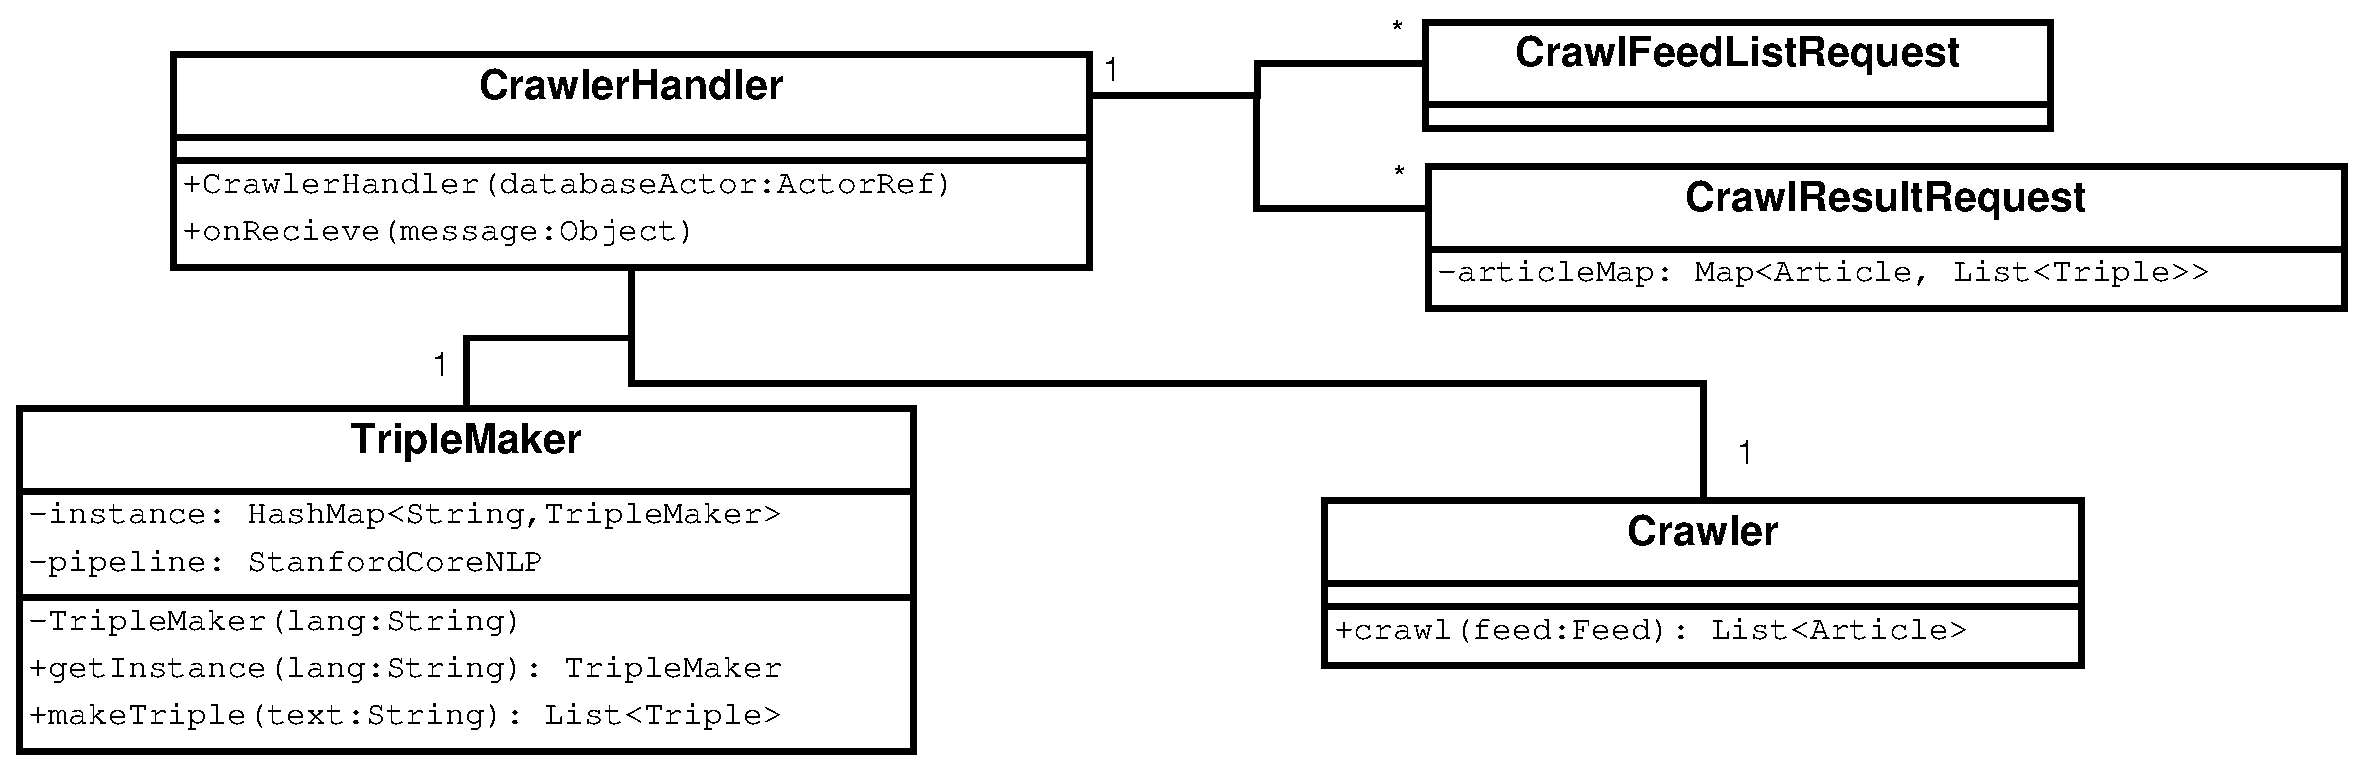
\includegraphics[width=1.03\textwidth]{Systementwurf/05_implementierungsentwurf/crawler-objekte}
\caption{Klassendiagramm für Komponente \ref{C10}}
\end{figure}
 
\subsection{Erläuterung}

Im Folgenden werden Attribute, Aufgaben und Kommunikationspartner für jede
Klasse der Serverkomponenten kurz erläutert. Triviale Methoden werden dabei
nicht berücksichtigt, sondern nur deren Attribute als \texttt{private} mit einem
Minuszeichen gekennzeichnet.

\begin{class}{40}{CrawlerHandler}
\item[Aufgabe]~\
Hauptklasse des Crawlers. Initialisierung der einzelnen Singleton-Objekte die
zum Bearbeiten eines Crawlvorgangs notwendig sind.
\item[Attribute]~\
\begin{itemize}
  \item \texttt{tripleMaker}: TripleMaker-Instanz
  \item \texttt{crawler}: Crawler-Instanz
  \item \texttt{databaseActor}: Akka-ActorRef-Objekt mit Verweis auf den
  DatabaseHandler
\end{itemize}
\item[Operationen]~\
\begin{itemize}
  \item \texttt{CrawlerHandler(ActorRef databaseActor)}:
  Instanziert die unter Attribute genannten Werte und sendet der
  Datenbank ein CrawlFeedListRequest. 
  \item \texttt{onRecive(Object message)}: Behandlet die eingehenden Messages:
\end{itemize}
\item[Kommunikationspartner]~\
  \textit{DatabaseHandler}
\end{class}

\begin{class}{40}{Crawler}
\item[Aufgabe]~\
Singleton-Klasse für das Crawlen der FeedList.
\item[Attribute]~\
keine
\item[Operationen]~\
\begin{itemize}
    \item \texttt{crawl(Feed feed)}: Crawlt von dem übergebenen Feed den Inhalt
    und lädt den Artikeltext.
\end{itemize}
\item[Kommunikationspartner]~\
\textit{CrawlerHandler}
\end{class}

\begin{class}{40}{TripleMaker}
\item[Aufgabe]~\
Singleton-Klasse für das Zerteilen der Artikeltexte in Triple für die Datenbank.
\item[Attribute]~\
\begin{itemize}
  \item \texttt{instance}: \texttt{TripleMaker}-Instanz für die verschiedenen 
  \item \texttt{pipeline}: \texttt{StandfortCoreNLP}-Instanz
  \item \texttt{lang}: Speichert die Sprache für die Triplezerlegung
\end{itemize}
\item[Operationen]~\
\begin{itemize}
    \item \texttt{TripleMaker(String lang)}: Instanziert die texttt{pipeline}
    mit den passenden Spracheinstellungen.
    \item \texttt{getInstance(String lang)}: Instanziert den texttt{TripleMaker}
    oder gibt eine schon bestehende Instanz zurück.
    \item \texttt{makeTriple(String text)}: Zerlegt den übergebenen Text in
    Triple.
\end{itemize}
\item[Kommunikationspartner]~\
\textit{CrawlerHandler}
\end{class}

\begin{class}{40}{CrawlFeedListRequest}
\item[Aufgabe]~\
Objekt zur Anfrage auf Erhalt der Feedliste.
\item[Attribute]~\
keine
\item[Operationen]~\
keine
\item[Kommunikationspartner]~\
\textit{DatabaseHandler}
\end{class}

\begin{class}{40}{CrawlResultRequest}
\item[Aufgabe]~\
Objekt zur Anfrage auf Aktualisierung der Datenbank.
\item[Attribute]~\
\begin{itemize}
  \item \texttt{articleMap}: Liste mit Artikeln der
  Feeds und den Triple aus den Texten.
\end{itemize}
\item[Operationen]~\
keine
\item[Kommunikationspartner]~\
\textit{DatabaseHandler}
\end{class}

\FloatBarrier

\section{Implementierung von Komponente $\langle$C50$\rangle$: Query-Processor}

Der QueryProcessor ist das Herzstück des \NewsGenies. Hier werden vom Benutzer
gestellte Fragen analysiert und erkannt, um anschließend dementschende Anfragen
an die Datenbank zu stellen. Die Ergebnisse
einer Suche werden dann für den Benutzer aufbereitet
und anschließend zum Client zurückgeschickt.

\subsection{Paket-/Klassendiagramm}

\begin{figure}[ht]
\centering
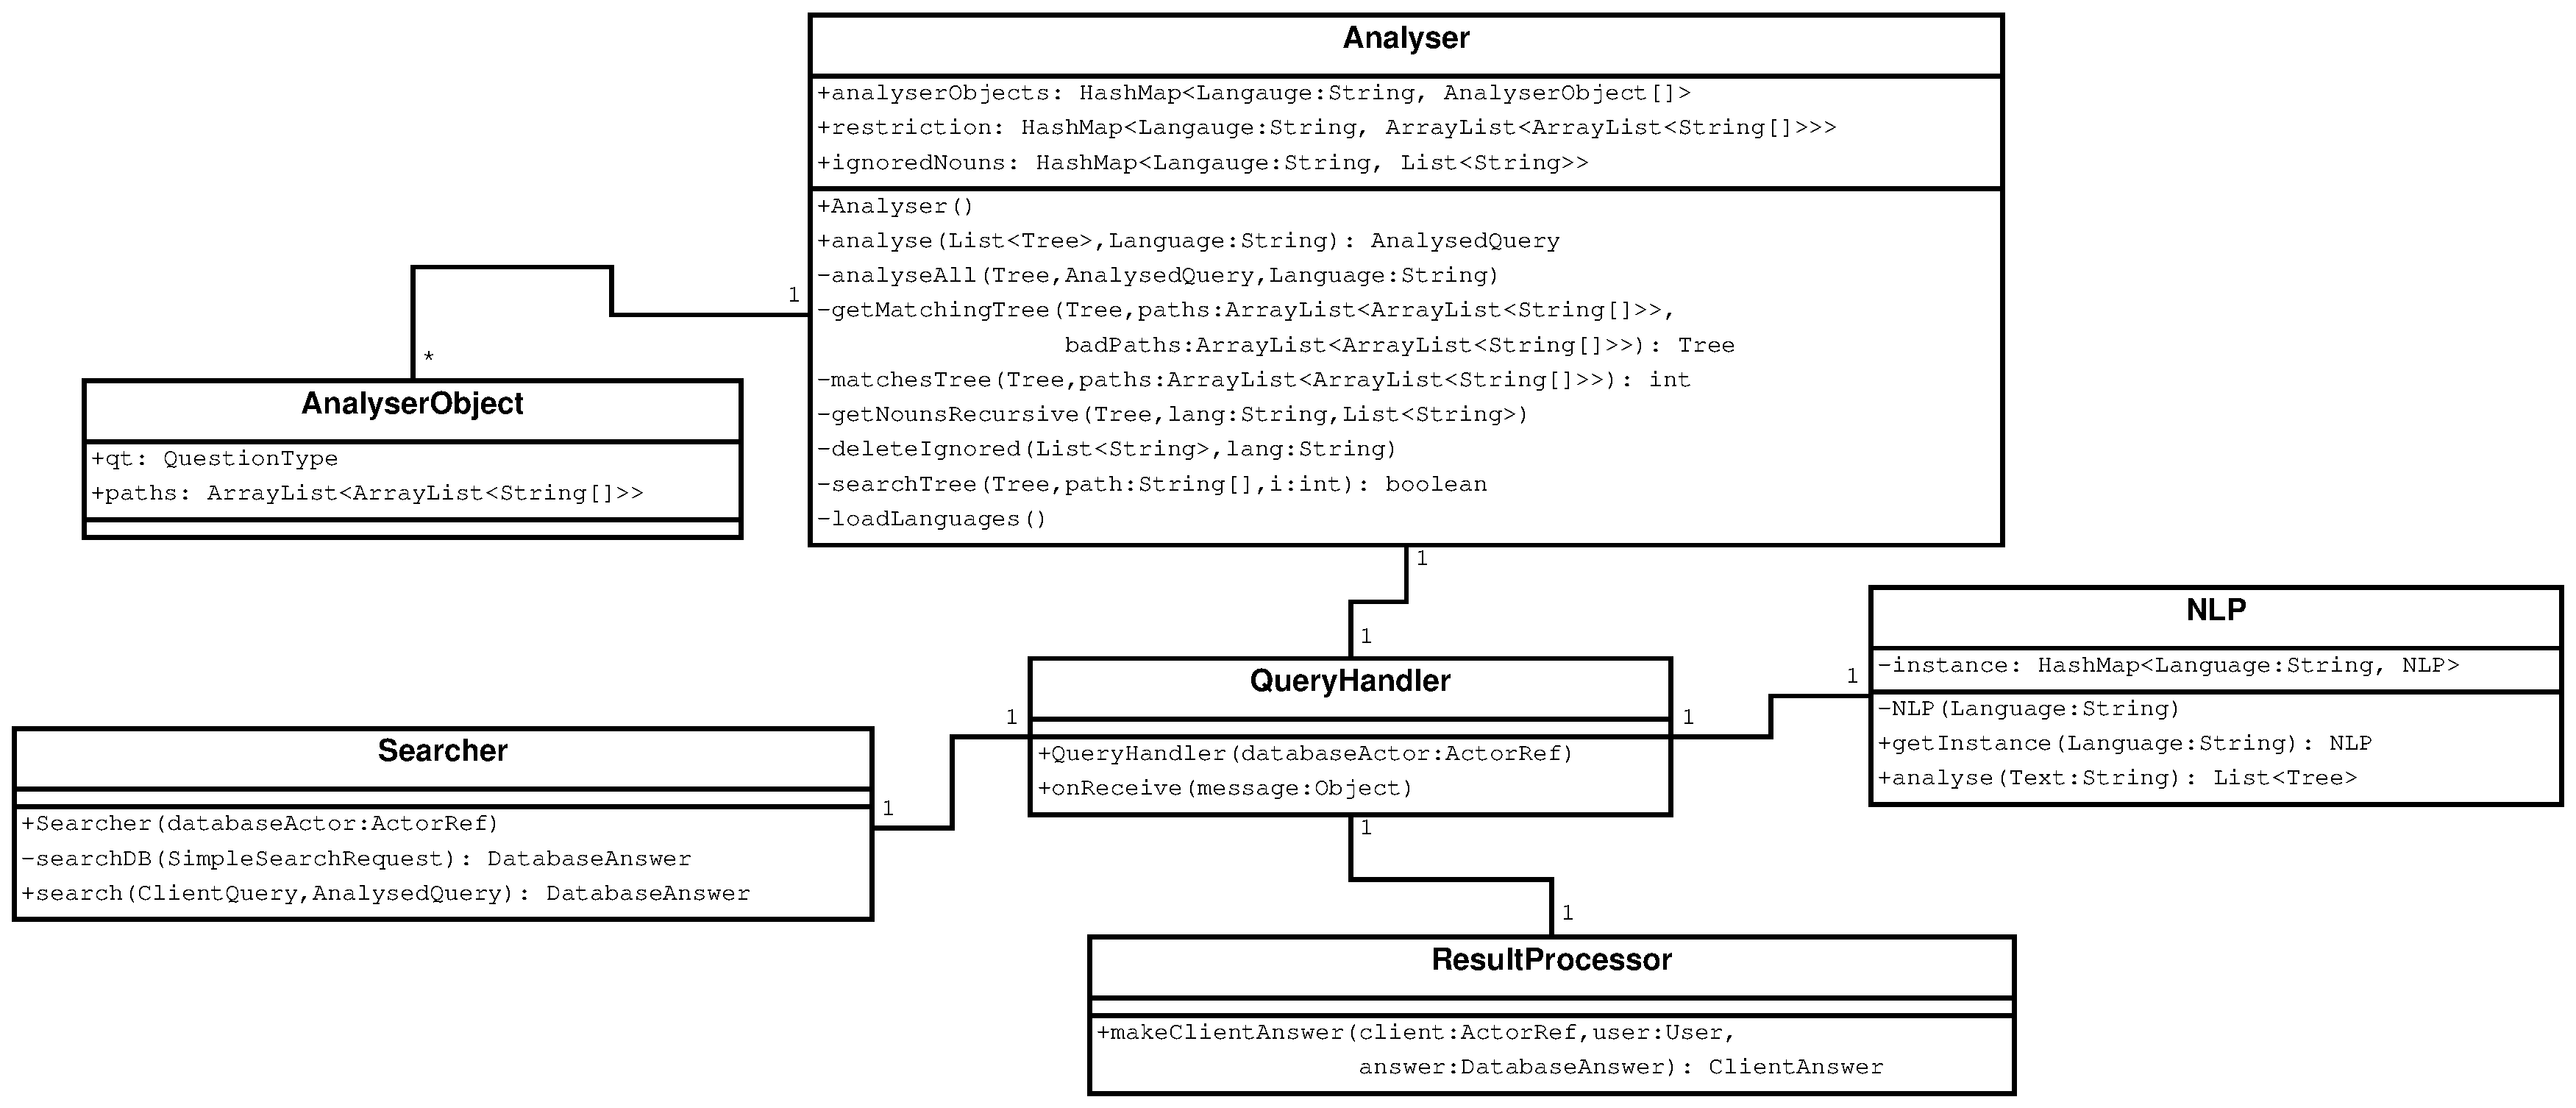
\includegraphics[width=1\textheight, angle=90]{Systementwurf/05_implementierungsentwurf/Diagramm1}
\caption{Klassendiagramm für Komponente \ref{C50}}
\end{figure}
 
\FloatBarrier

\subsection{Erläuterung}

Im Folgenden werden Attribute, Aufgaben und Kommunikationspartner für jede
Klasse der Serverkomponenten kurz erläutert. Triviale Methoden werden dabei
nicht berücksichtigt.

\begin{class}{50}{Analyser}
\item[Aufgabe]~\
Analysiert Wortbäume mit Suchmustern, durch die die gestellte Frage erkannt
werden kann.
\item[Attribute]~\
\begin{itemize}
\item \texttt{analyserObjects}: \texttt{HashMap<String, AnalyserObject[]>}:
Enthält zu einer Sprache AnalyserObjects.
\item \texttt{restriction}: \texttt{HashMap<String,
ArrayList<ArrayList<String[]>>>}: Enthält für eine Sprache Suchmuster für Restriktionen.
\item \texttt{ignoredNouns}: \texttt{HashMap<String, List<String>>}: Enthält
für eine Sprache eine Liste mit Wörter die ignoriert werden sollen.
\end{itemize}
\item[Operationen]~\
\begin{itemize}
\item \texttt{Analyser()}: Erstellt eine Instanz des Analysers.
\item \texttt{analyse(List<Tree> treeList)}: Analysiert eine Wort-Baum-Liste.
\item \texttt{analyseAll(Tree tree, AnalysedQuery analysedQuery, String lang)}:
Findet für einen gegebenen Wort-Baum eines Satzes in einer Sprache den Fragetyp und Schlüsselwörter heraus.
\item \texttt{getMatchingTree(Tree tree, ArrayList<ArrayList<String[]>> paths,
ArrayList<ArrayList<String[]>> badPaths)}: Sucht mithilfe eines gegebenen
Musters nach einer Struktur im Baum und gibt diese aus.
\item \texttt{matchesTree(Tree tree, ArrayList<ArrayList<String[]>> paths)}:
Prüft, ob ein Baum mit einem gegeben Muster übereinstimmt.
\item \texttt{getNounsRecursive(Tree tree, String lang, List<String> list)}:
Suche alle Nomen aus einem Baum heraus und fügt diese in eine Liste ein.
\item \texttt{deleteIgnored(List<String> list, String lang)}: Entfernt alle zu
ignorierende Wörter aus einer Liste.
\item \texttt{searchTree(Tree tree, String[] path, int i)}: Prüft, ob ein
gegebener Such-Pfad im Baum existiert.
\item \texttt{loadLanguages()}: Ließt Suchmuster einer Sprache in
AnalyserObject ein.
\end{itemize}
\item[Kommunikationspartner]~\
\textit{QueryHandler}
\end{class}

\begin{class}{50}{AnalysedObject}
\item[Aufgabe]~\
Enthält einen Fragetyp und ein Suchmuster, mit dem man den Fragetyp
identifizieren kann.
\item[Attribute]~\
\begin{itemize}
\item \texttt{qt}: \texttt{QuestionType} Der Fragetyp.
\item \texttt{paths}: \texttt{ArrayList<ArrayList<String[]>>} Das Suchmuster.
\end{itemize}
\item[Operationen]~\
keine
\item[Kommunikationspartner]~\
\textit{Analyser}
\end{class}

\begin{class}{50}{Searcher}
\item[Aufgabe]~\
Kommuniziert mit der Datenbank.
\item[Attribute]~\
keine
\item[Operationen]~\
\begin{itemize}
\item \texttt{Searcher(ActorRef databaseActor)}: Instanziert den Searcher
\item \texttt{search(Messages.ClientQuery originalQuery, AnalysedQuery aq)}:Sucht entsprechend der Fragestellung nach Ergebnissen.
\item \texttt{searchDB(SimpleSearchRequest simpleSearchRequest)}: Stellt anfragen an die Datenbank.
\end{itemize}
\item[Kommunikationspartner]~\
\textit{DatabaseHandler}, \textit{QueryHandler}
\end{class}

\begin{class}{50}{QueryHandler}
\item[Aufgabe]~\
Der QueryHandler organisiert die Analyse der Querries.
\item[Attribute]~\
keine
\item[Operationen]~\
\begin{itemize}
	\item \texttt{QueryHandler(ActorRef databaseActor)}: Instanziiert den QueryHandler.
	\item \texttt{onReceive(Object message)}: Nimmt ClientQuery-Nachrichten entgegen, und lässt diese analysieren.
\end{itemize}
\item[Kommunikationspartner]~\
\textit{NLP}, \textit{ManagementHandler}, \textit{Searcher}, \textit{ResultProcessor}, \textit{Analyser}
\end{class}

\begin{class}{50}{NLP}
\item[Aufgabe]~\
Zerlegt Texte in Wort-Bäume, die der Analyser verarbeiten kann.
\item[Attribute]~\
\begin{itemize}
\item \texttt{instance}: \texttt{HashMap<String, NLP>} Enthält die NLP Instanz einer Sprache.
\end{itemize}
\item[Operationen]~\
\begin{itemize}
\item \texttt{NLP(String lang)}: Instanziiert NLP für eine gegebene Sprache.
\item \texttt{getInstance(String lang)}: Gibt die NLP-Instanz der jeweiligen
Sprache aus.
\item \texttt{analyse(String text)}: Analysiert einen Text bezüglich seiner
Sprache und erstellt daraus eine Wort-Baumstruktur, in der die Bedeutung der
einzelner Wörter steht.
\end{itemize}
\item[Kommunikationspartner]~\
\textit{QueryHandler}
\end{class}

\begin{class}{50}{ResultProcessor}
\item[Aufgabe]~\
Generiert aus vorgefertigten Textbausteinen und
Ergebnissen eine Antwort.
\item[Attribute]~\ keine
\item[Operationen]~\
\begin{itemize}
\item \texttt{makeClientAnswer(ActorRef client, User user, DatabaseAnswer
answer)}: Produziert aus einer SearchAnswer eine ClientAnswer.
\end{itemize}
\item[Kommunikationspartner]~\
\textit{QueryHandler}
\end{class}

%!TEX root = ../Systementwurf2.tex

\chapter{Datenmodell}

Zur dauerhaften Speicherung von Daten verwenden wir einen Virtuoso Triplestore. Dieser speichert Daten in Tripeln der Form (Subjekt, Prädikat, Objekt). In Diagramm~\ref{fig:6.1} wird das Prädikat durch einen Pfeil, der vom Subjekt zum Objekt führt, dargestellt. Rechtecke repräsentieren Literale und Ellipsen URIs. Das Präfix \glqq ng:\grqq\ deutet gemäß dem RDF-Standard an, dass Daten, die dieses enthalten, in URI-Form gespeichert werden. Unterstrichene Sub- und Objekte speichern ihren tatsächlichen Namen aus dem Diagramm. Bei nicht unterstrichenen Feldern soll der Name anzeigen, was sie später enthalten. Von den Prädikaten speichern alle bis auf \glqq ng:Predicate\grqq\ ihren Namen.\\
Die Menge aller gespeicherten Tripel bildet den sogenannten RDF-Graphen.\\
Es gibt vier Datentypen, die in der Datenbank gespeichert werden. Diese werden im Folgenden vorgestellt.\\
Der Wet nach jedem Tripel, gibt an, wieviele solche Relationen ein Subjekt haben kann.
\begin{description} 
\item[User:] Ein User-Datensatz repräsentiert einen Benutzer des Systems und besteht aus den folgenden Tripeln:
\begin{itemize}
  \item (UserId, isType, User) (1): Weißt den Datensatz als Benutzer aus.
  \item (UserId, hasName, Name) (1) (unique): Enthält den Namen des Benutzers.
  \item (UserId, hasPassword, Password) (1): Enthält das gehashte Passwort des Benutzers.
  \item (UserId, hasEmail, E-Mail) (1) (unique): Enthält die E-Mail-Adresse des Benutzers.
  \item (UserId, registeredAt, Date) (1): Enthält das Datum der Registration des Benutzers.
  \item (UserId, loggedInAt, Date) (1): Enthält das Datum des letzten Logins des Benutzers.
  \item (UserId, isAdmin, isAdmin) (1): Speichert, ob der Benutzer Administratorenrechte besitzt.
  \item (UserId, hasLanguage, Language) (1): Speichert die vom Nutzer gewählte Sprache.
  \item (UserId, reads, FeedId) (0...n): Speichert, welche Feeds der Benutzer abonniert hat.
\end{itemize}
\item[Feed:] Ein Feed-Datensatz repräsentiert einen RSS-Feed und besteht aus den folgenden Tripeln:
\begin{itemize}
  \item (FeedId, isType,Feed) (1): Weißt den Datensatz als Feed aus.
  \item (FeedId, hasTitle, Title) (1): Enthält den Titel des Feeds.
  \item (FeedId, hasURL, URL) (1) (unique): Enthält die URL, unter der der RSS-Feed zu finden ist.
  \item (FeedId, addedAt, Date) (1): Enthält das Erstellungsdatum des Feeds.
  \item (FeedId, hasLanguage, Language) (1): Speichert, die Sprache des Feeds.
  \item (FeedId, inCategory, Category) (0...n): Speichert die Kategorien des Feeds.
\end{itemize}
\item[Article:] Ein Article-Datensatz repräsentiert einen Nachrichtenartikel und besteht aus den folgenden Tripeln:
\begin{itemize}
  \item (ArticleId, isType, Article) (1): Weißt den Datensatz als Nachrichtenartikel aus.
  \item (ArticleId, hasTitle, Title) (1): Enthält die Überschrift des Artikels.
  \item (ArticleId, hasDescription, Abstract) (1): Enthält eine einführende Beschreibung des Artikels, falls eine solche existiert.
  \item (ArticleId, hasText, Text) (1): Enthält den Text des Artikels.
  \item (ArticleId, publishedAt, Date) (1): Enthält das Datum der Veröffentlichung des Artikels.
  \item (ArticleId, hasAuthor, Author) (0...n): Enthält die Namen der Autoren des Artikels.
  \item (ArticleId, hasTopic, Topic) (0...n): Speichert die Themen, die der Artikel behandelt.
  \item (ArticleId, hasSentence, Subject) (0...n): Speichert Referenzen auf die Satztripel aus dem Artikel.
  \item (ArticleId, publishedIn, FeedId) (1): Speichert in welchem Feed der Artikel veröffentlicht wurde.
\end{itemize}
Um eine effiziente Volltextsuche auf den Artikeln zu ermöglichen, wird für diese zusätzlich eine Indexstruktur mit Hilfe von Apache Lucene erzeugt.
\item[Sentence:] Ein Sentence-Datensatz repräsentiert einen (Teil-) Satz der in einem der Artikel vorkommt. Dieser wird in Subjekt, Prädikat und Objekt aufgeteilt und besteht aus einem einzigen Tripel:
\begin{itemize}
  \item (Subject, Predicate, Object): Ein aufgeteilter Satz.
\end{itemize}
Diese aus dem Artikel extrahierten Sätze werden verwendet, um Nutzeranfragen möglichst genau zu verarbeiten.
\end{description}

Zusätzlich zu diesen Daten spiegeln wir noch einen LinkedOpenData-Graphen in unserer Datenbank, um schnelle Zugriffszeiten auf diesen zu garantieren.

\pagebreak
\section{Diagramm} 

\begin{figure}[ht]
\centering
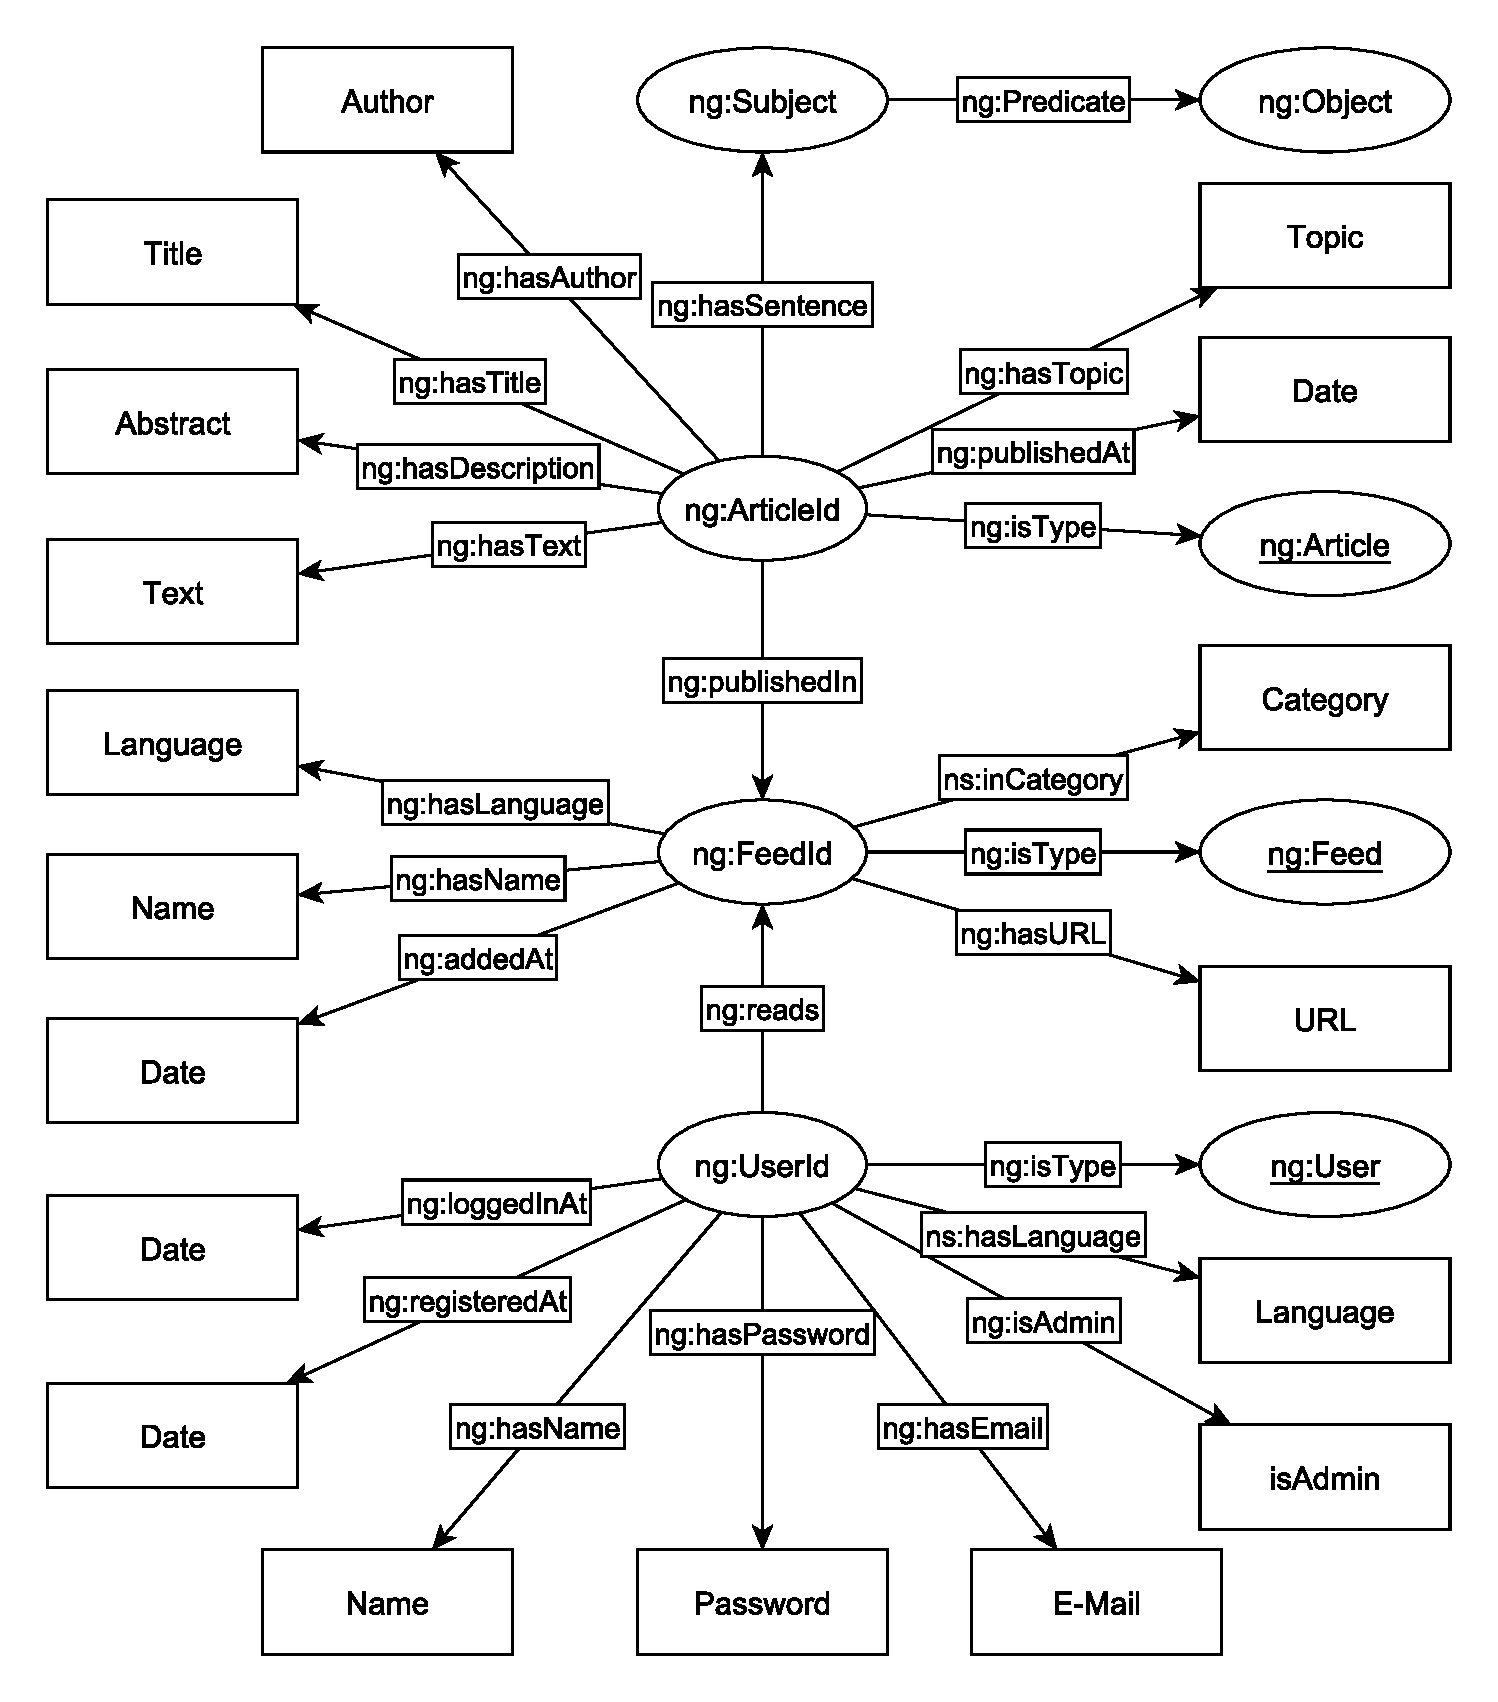
\includegraphics[width=0.90\textwidth]{Systementwurf/datenmodell/DBDiagramm.eps}
\caption{Datenbankdiagramm}
\label{fig:6.1}
\end{figure}
\section{Erläuterung}

Da wir einen Triplestore verwenden, gibt es keine wirklichen Entitäten und auch innerhalb der einzelnen Datensätze gibt es Verknüpfungen mit Kardinalität \( \neq\) 1. Die Kardinalitäten der Verknüpfungen innerhalb der Datensätze sind oben aufgeführt.

\begin{entity}{10}{User}
\begin{tabular}[ht]{|l|l|}
  \hline
  Beziehung & Kardinalität\\
  \hline
  reads & 0...n\\
  \hline
\end{tabular}
\end{entity}

\begin{entity}{20}{Artikel}
\begin{tabular}[ht]{|l|l|}
  \hline
  Beziehung & Kardinalität\\
  \hline
  publishedIn & 1\\
  \hline
  hasSentence & 0...n\\
  \hline
\end{tabular}
\end{entity}
%!TEX root = ../Systementwurf2.tex

% Kapitel 5
%-------------------------------------------------------------------------------
\chapter{Serverkonfiguration}

Der Server besteht insgesamt aus drei Komponenten, die jeweils einzeln gestartet und konfiguriert werden können. Der Server ist dazu konzipiert, auf einem Linux-System zu laufen.

\section{Virtuoso}

Zur Zeit der Auslieferung verwenden wir Virtuoso 6.1 in der opensource Variante. 
Virtuoso kann von \texttt{http://virtuoso.openlinksw.com/dataspace/doc/dav/wiki/Main/VOSDownload} heruntergeladen werden.

Die Konfigurationsdatei heißt \texttt{virtuoso.ini} und liegt standardmäßig im Verzeichnis \texttt{/etc/ $\hookleftarrow$""virtuoso-opensource-\%version\%/}.
In dieser Datei können insbesondere die Ports der Datenbank (standardmäßig 1111) und des Datenbankbackends (standardmäßig 8890) und der Ort, an dem die Virtuoso-Systemdateien liegen, (standardmäßig \texttt{/var/lib/virtuoso-opensource- $\hookleftarrow$""\%version\%/db/}) festgelegt werden.\\
Die ausführbare Datei heißt \texttt{virtuoso-t} und liegt in \texttt{/usr/bin/}. Zum Starten der Datenbank muss der Pfad der Konfiguration angegeben werden. Der Aufruf sieht dementsprechend folgendermaßen aus: \texttt{virtuoso-t [+foreground] +configfile /etc/virtuoso-opensource-~$\hookleftarrow$\linebreak\%version\%/virtuoso.ini}.

\section{Newsgenie-Server}

Der Newsgenie-Server ist eine Java-Anwendung und wird als ausführbares Jar-Archiv ausgeliefert. Es wird eine Java-Installation der Version 7 oder höher benötigt. Die Konfigurationsdatei heißt \texttt{server.cfg} und muss sich im gleichen Ordner wie die Jar-Datei befinden. In der Konfiguration können die Server-IP-Adresse sowie der Akka- und der Virtuoso-Port festgelegt werden. Die Server-IP muss mit der wirklichen IP des Servers übereinstimmen und der Virtuoso-Port muss dem Port entsprechen, auf dem Virtuoso Anfragen entgegennimmt (siehe oben).\\
Der Server kann mittels \texttt{java -jar server.jar} gestartet werden. Hierzu ist es notwendig, dass die Datenbank bereits läuft und erreichbar ist.

\section{Webinterface}

Das Webinterface ist eine Play-Anwendung. Das Play-Framework kann von  \texttt{http://www.play~$\hookleftarrow$\linebreak framework.com/download} heruntergeladen werden. Danach kann das Webinterface mittels \texttt{play run} gestartet werden. Um das Webinterface auszuführen, müssen sowohl Datenbank als auch Server laufen. Die Konfigurationsdatei heißt \texttt{application.conf} und liegt im Unterordner \texttt{./conf/}. Hier kann zum Beispiel die IP-Adresse geändert werden.
%!TEX root = ../Systementwurf.tex

\chapter{Erfüllung der Kriterien}

In diesem Abschnitt wird beschrieben, wie die im Pflichtenheft aufgeführten Kriterien erfüllt
werden und worauf geachtet wird. Es wird zuerst auf die Musskriterien, dann auf die Soll und Kann-Kriterien und zuletzt auf die Abgrenzungskriterien eingegangen.


\section{Musskriterien}

Die folgenden Kriterien sind unabdingbar und müssen durch das Produkt erfüllt
werden:

\ref{RM1} Ein- und Ausgabe in natürlicher Sprache

Die Spracheingabe erfolgt durch ein am Raspberry Pi angebrachtes Mikrofon. Der \textit{Client}\ref{C10} nimmt gesprochene Sprache auf und wandelt diese mithilfe der Google-Speech-Api in Text um.
Auf dem Server wird der Text dann im \textit{Query-Processor}\ref{C50} mithilfe von Natural Language Proccessing und Named Entity Recognition analysiert und erkannt.
Die Sprachausgabe erfolgt durch einem Lautsprecher am Raspberry Pi. Der \textit{Client}\ref{C10} erhält auszugebendes als Text, wandelt es in Sprache um und gibt es anschließend aus.

\ref{RM2} Interaktives Verhalten

Durch drücken des Aufnahmeknopfes während einer Sprachausgabe, kann der Nutzer diese unterbrechen, um seine vorherige Suchanfrage noch weiter zu spezifizieren oder negatives Feedback (z.B. "`Stop"') zu geben.
Falls der \textit{Query-Processor}\ref{C50} eine Anfrage nicht klar verstehen konnte, kann der \textit{Client}\ref{C10} dem Nutzer eine Reihe von vordefinierten Ja/Nein Fragen stellen, um die Anfrage einzugrenzen.

\ref{RM3} Das System muss die englische Sprache unterstützen

\NewsGenie ist standardmäßig auf die englische Sprache eingestellt.
Jeder Nutzer kann am \textit{Webinterface}\ref{C20} einstellen, welche Sprache er verwenden möchte. 
Alle für die Lokalisierung verantwortlichen Inhalte werden in externe Textdateien verlagert, was das einbauen weiterer Sprachen stark vereinfacht.
Jeder Artikel in der \textit{Datenbank}\ref{C30} erhält einen Sprach-Tag, um zu
gewährleisten, dass jeder Nutzer nur Artikel seiner eingestellten Sprache entsprechend erhält.
Jegliche von uns verwendete Fremdanbietersoftware unterstützt auch standardmäßig die englische Sprache.

\pagebreak

\ref{RM4} Benutzerschnittstelle

Das \textit{Webinterface}\ref{C20} wird mit Hilfe des Play-Frameworks auf dem Server umgesetzt.

\ref{RM5} Backend

Artikel werden als Tripel in der \textit{Datenbank}\ref{C30} gespeichert und durch Lucene zur Suche aufbereitet.
Außerdem erhalten Artikel zusätzlich einen Zeitstempel um das Erkennen von veralteten Artikeln zu ermöglichten.

\section{Sollkriterien}

Die Erfüllung folgender Kriterien für das abzugebende Produkt wird angestrebt:

\ref{RS1} Entitäts-Erkennung

Mit dem Named Entity Recognizer aus Stanford NLP können Entitäten in gecrawlten Artikeln erkannt werden. 
Anschließend werden diese in der \textit{Datenbank}\ref{C30} abgelegt und durch die Tripelspeicherweise miteinander verknüpft. 
Dieses Verknüpfen ermöglicht es, Zusammenhänge zwischen Artikeln besser zu erkennen um so eine höhere Antwortqualität 
zu erreichen.

\ref{RS2} News Crawling

Der Crawler durchsucht regelmäßig die RSS-Feed-Quellen nach neuen Artikeln und speist diese anschließend in die \textit{Datenbank}\ref{C30} ein.
Neue Quellen können sowohl im \textit{Webinterface}\ref{C20} als auch per Spracheingabe am \textit{Client}\ref{C10} dynamisch dem Crawler hinzugefügt werden.

\ref{RS3} Deutsche Sprache

Die deutsche Sprache wird vollkommen unterstützt.
Auch die von uns verwendete Fremdanbietersoftware unterstützt die deutsche Sprache.

\ref{RS5} Persönlichkeit

Der \textit{Client}\ref{C10} kann rudimentäre Fragen wie z.B. {\glqq Hi, how are
you?\grqq} stellen, sowie auf einer kleinen Anzahl von Spaßfragen wie z.B.
{\glqq What does the Fox say?\grqq}  antworten.

\section{Kannkriterien}

Die Erfüllung folgender Kriterien für das abzugebende Produkt wird angestrebt:

\ref{RC1} Konkurrentes News-Crawling

Das Crawling findet auf dem Server in einem separatem Prozess statt, weswegen es die normalen Funktionen von \NewsGenie nicht beeinträchtigt.

\ref{RC2} Trend-Erkennung

Trends können auf zwei Arten gefunden werden:
Zum einem durch die Analyse, wie häufig welche Themen von Nutzern abgefragt wurden, 
und zum anderen beim crawlen, wenn zu einem Zeitpunkt bestimmte Themen besonders häufig in unterschiedlichen RSS-Feeds auftauchen.

\ref{RC3} Personalisierung

Zu jedem Nutzer werden in der \textit{Datenbank}\ref{C30} Nutzerdaten inklusive seiner Suchhistorie gespeichert.
Aus der Häufigkeit des Vorkommens von bestimmen Themen in der Suchhistorie eines Nutzers können dessen Interessen abgeleitet werden.

\section{Abgrenzungskriterien}

Folgende Funktionalitäten werden nicht durch das Produkt, sondern wie folgt
beschrieben anderweitig erfüllt

\ref{RW1} Das System soll die Sprachen nicht automatisch unterscheiden können

Der Nutzer kann am \textit{Webinterface}\ref{C20} die Sprache einstellen (Deutsch und Englisch).

\ref{RW2} Das System soll keine komplexen Fragen stellen

Zu komplexe Fragen mit vielen Nebensätzen sind äußerst schwer zu erkennen, was den Umfang dieses Praktikums 
übertreffen würde.
Des Weiteren genügen in den meisten Fällen einfache Fragen, um auszudrücken wonach man sucht.

\ref{RW3} Das System umfasst keine künstliche Intelligenz, Antworten werden
nicht umformuliert

Artikel werden in eine Auswahl von vordefinierten Sätzen eingepackt, aber sonst unverändert ausgeben, um dennoch natürlich wirken zu können.

\ref{RW4} Artikel, die nicht im RSS-Feed verlinkt sind, werden nicht
verarbeitet

Da fast jede Nachrichtenseite im Internet einen RSS-Feed anbietet, ist die Wahrscheinlichkeit groß, dass sich das gesuchte Thema in den dort verlinkenden Artikeln befindet.
%!TEX root = ../Pflichtenheft.tex

\chapter{Glossar}

\begin{description}

\item[Account] Benutzerkonto, dient zur Identifizierung eines Benutzers und
speichert benutzerspezifische Daten.

\item[Administrator] Ein Benutzer mit besonderen Rechten zur Verwaltung von
anderen Benutzern und Ressourcen eines Systems.

\item[API] Programmierschnittstelle, wird von einem Programm zur Anbindung von
weiteren Programmteilen auf Quelltextebene zur Verfügung gestellt. 

\item[Backend] Für den Benutzer nicht sichtbarer Programmteil, läuft
typischerweise auf einem Server und stellt Daten für eine Clientapplikation zur
Verfügung.

\item[Client] Nutzer einer von einem Server über das Netzwerk angebotenen
Ressource.

\item[Crawler] Ein Serverdienst im Backend zur Erfassung und Verarbeitung von
Daten aus verschiedenen Quellen.

\item[Datenbank] Ein Programm zur strukturierten Datenhaltung mit definierter
Abfragesprache.

\item[Flac] \emph{Free Lossless Audio Codec}, eine verlustfreie Komprimierungsmethode
für Audiodateien.

\item[Hash] Eine Prüfsumme, oft mit festgelegter Länge, die zur
eindeutigen Identifizierung von Datensätzen oder für kryptografische Zwecke
eingesetzt wird.

\item[Prozedur] Ein Verfahren mit festgelegter Befehlsreihenfolge zur
planmäßigen Lösung von Problemen. Bezeichnet in der Programmierung oft einen
Codeblock oder eine Funktion für eine bestimmte Aufgabe.

\item[Raspberry Pi] Günstiger Einplatinencomputer mit geringer
Leistungsaufnahme.

\item[RSS-Feed] Abkürzung für Really Simple Syndication-Feed, einfaches und
strukturiertes Format zur Veröffentlichung von Änderungen auf Webseiten. 
Ein RSS-Feed versorgt den Benutzer mit kurzen Informationsblöcken wie 
Nachrichtentitel und Textanriss, ähnlich einem Newsticker.

\item[Server] Ein Computer der zentrale Dienste in einem Netzwerk für mehrere
Nutzer zur Verfügung stellt. 

\item[String] Eine Folge von Zeichen (Zeichenkette) von definierten Symbolen und
fester oder variabler Länge.

\item[Query] bezeichnet eine Abfrage, oft an eine Datenbank oder
Serveranwendung, die häufig einen formalen Ausdruck erwartet.

\item[Query-Processor] Serverapplikation zur Beantwortung von Querys. Läuft im
Backend der Anwendung.

\item[Webinterface] Benutzerschnittstelle auf Basis einer Webseite, erlaubt die
Eingabe von Daten durch den Benutzer und gibt Rückmeldung über Erfolg/Misserfolg
der getätigten Einstellungen.

\end{description}


%------Ende des Dokumentes------------------------------------------------------
\end{document}
